\documentclass{article}
\usepackage[margin=1in]{geometry}
\usepackage{amsmath}
\usepackage{amssymb}
\usepackage{booktabs}
\usepackage{tikz}
\usetikzlibrary{positioning, arrows.meta, shapes.geometric, calc, decorations.pathreplacing, decorations.markings}

\begin{document}

\title{Disturbance Rejection Capability:\\Maximum Allowable Speed Analysis}
\author{}
\date{}
\maketitle

% =============================================================================
\section{Understanding the Control System}
% =============================================================================

\subsection{What is the ``Disturbance''?}

In this radar system, the target motion causes a Doppler phase shift, which is treated as the disturbance that the controller must cancel.

% TikZ: Disturbance Concept Box
\begin{figure}[h]
\centering
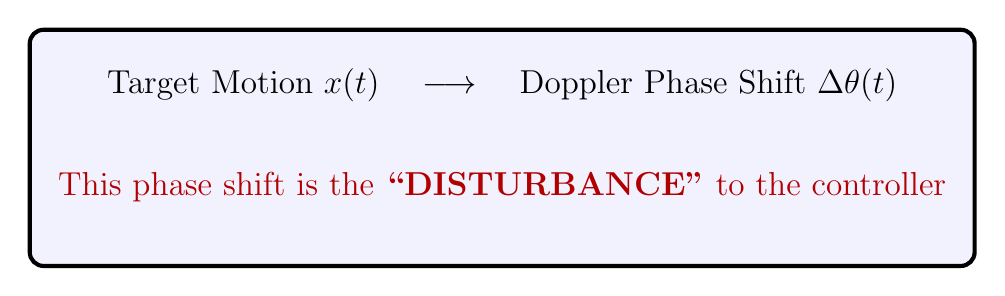
\begin{tikzpicture}[
    box/.style={rectangle, draw=black, line width=1.5pt, rounded corners=5pt, 
                minimum width=12cm, minimum height=3cm, fill=blue!5},
    arrow/.style={-{Stealth[length=4mm, width=3mm]}, line width=1.5pt}
]
    % Main box
    \node[box] (main) at (0,0) {};
    
    % Content
    \node[font=\large] at (0, 0.8) {Target Motion $x(t)$ \quad $\longrightarrow$ \quad Doppler Phase Shift $\Delta\theta(t)$};
    \node[font=\large, text=red!70!black] at (0, -0.5) {This phase shift is the \textbf{``DISTURBANCE''} to the controller};
    
\end{tikzpicture}
\caption{The disturbance in the radar control system.}
\end{figure}

The Doppler phase shift is given by:
\begin{equation}
\Delta\theta(t) = \frac{4\pi}{\lambda} x(t)
\end{equation}

% =============================================================================
\subsection{What Does the Controller Do?}

\textbf{Goal:} Keep $\theta = \pi$ (the desired operating point)

% TikZ: Control System Block Diagram
\begin{figure}[h]
\centering
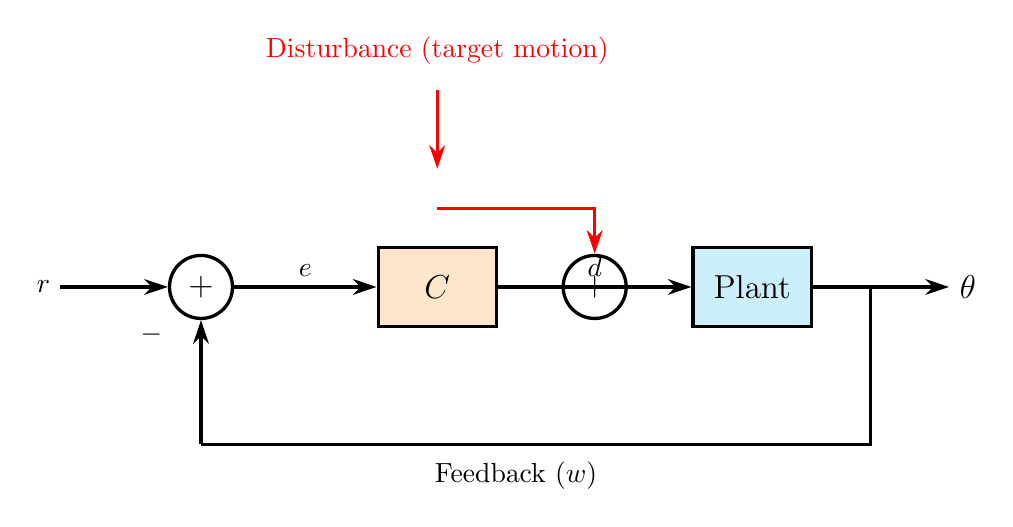
\begin{tikzpicture}[
    block/.style={rectangle, draw=black, line width=1.2pt, minimum width=1.5cm, 
                  minimum height=1cm, font=\large},
    sum/.style={circle, draw=black, line width=1.2pt, minimum size=0.8cm, font=\large},
    arrow/.style={-{Stealth[length=3mm, width=2mm]}, line width=1.2pt},
    label/.style={font=\normalsize}
]

    % Disturbance arrow
    \node[font=\normalsize, text=red] at (3, 3) {Disturbance (target motion)};
    \draw[arrow, red] (3, 2.5) -- (3, 1.5);
    
    % Sum block
    \node[sum] (sum) at (0, 0) {$+$};
    \node[label, below left=0.1cm of sum] {$-$};
    
    % Controller
    \node[block, fill=orange!20] (ctrl) at (3, 0) {$C$};
    
    % Plant
    \node[block, fill=cyan!20] (plant) at (7, 0) {Plant};
    
    % Input
    \node[label] (r) at (-2, 0) {$r$};
    \draw[arrow] (r) -- (sum);
    
    % Sum to Controller
    \draw[arrow] (sum) -- (ctrl) node[midway, above] {$e$};
    
    % Controller to Plant
    \draw[arrow] (ctrl) -- (plant) node[midway, above] {$d$};
    
    % Output
    \draw[arrow] (plant) -- ++(2.5, 0) node[right, font=\large] {$\theta$};
    
    % Feedback
    \draw[line width=1.2pt] (8.5, 0) -- (8.5, -2) -- (0, -2);
    \draw[arrow] (0, -2) -- (sum);
    \node[label] at (4, -2.4) {Feedback ($w$)};
    
    % Disturbance input to sum before plant
    \node[sum] (sum2) at (5, 0) {$+$};
    \draw[arrow, red] (3, 1) -- (5, 1) -- (sum2);
    
\end{tikzpicture}
\caption{Control system block diagram with disturbance.}
\end{figure}

\begin{itemize}
    \item $r = 0$: Set-point (desired frequency shift = 0, meaning $\theta = \pi$)
    \item \textbf{Disturbance}: Doppler phase shift from target motion
    \item \textbf{Controller output} $d$: Tunable delay that cancels the disturbance
\end{itemize}

% =============================================================================
\section{Why Maximum Speed = Disturbance Rejection?}
% =============================================================================

\subsection{The Faster the Target Moves $\rightarrow$ The Larger the Disturbance Rate}

\begin{table}[h]
\centering
\renewcommand{\arraystretch}{1.5}
\begin{tabular}{lcc}
\toprule
\textbf{Target Speed} & \textbf{Phase Change Rate} & \textbf{Controller Difficulty} \\
\midrule
Slow & Small $\frac{d\theta}{dt}$ & Easy to track \\
Fast & Large $\frac{d\theta}{dt}$ & Hard to track \\
Too Fast & Controller can't keep up & \textcolor{red}{\textbf{Loses lock!}} \\
\bottomrule
\end{tabular}
\caption{Relationship between target speed and controller difficulty.}
\end{table}

\subsection{Mathematical Relationship}

Target moving at constant speed $v$:
\begin{equation}
x(t) = v \cdot t
\end{equation}

Phase shift:
\begin{equation}
\Delta\theta(t) = \frac{4\pi}{\lambda} \cdot v \cdot t = \frac{2\omega_n}{c} \cdot v \cdot t
\end{equation}

\textbf{Rate of phase change:}
\begin{equation}
\frac{d(\Delta\theta)}{dt} = \frac{2\omega_n \cdot v}{c}
\end{equation}

The faster the target ($v \uparrow$), the faster the phase changes, and the harder it is for the controller to cancel!

% =============================================================================
\section{Phase Error Analysis}
% =============================================================================

\subsection{What Happens When Controller Can't Keep Up?}

The controller tries to regulate $\theta$ to $\pi$, but has limited bandwidth $\omega_{BW}$.

\textbf{Phase error} $e = \theta - \pi$ accumulates when:
\begin{equation}
\text{Disturbance rate} > \text{Controller bandwidth}
\end{equation}

\subsection{Steady-State Phase Error}

From the paper (equation 17):
\begin{equation}
\lim_{t \to \infty} e(t) = \frac{2v\omega_n}{c \cdot \omega_{BW}}
\end{equation}

\begin{table}[h]
\centering
\renewcommand{\arraystretch}{1.5}
\begin{tabular}{lcc}
\toprule
\textbf{Speed} $v$ & \textbf{Phase Error} $e$ & \textbf{Result} \\
\midrule
Low & Small & $\checkmark$ Good tracking \\
Medium & Moderate & $\sim$ Some error \\
High & Large ($> 0.4\pi$) & $\times$ \textcolor{red}{System unstable!} \\
\bottomrule
\end{tabular}
\caption{Effect of speed on phase error and system stability.}
\end{table}

% =============================================================================
\section{Stability Limit}
% =============================================================================

\subsection{Region of Stability: $\theta \in (0.5\pi, 1.5\pi)$}

% TikZ: Plant Gain vs Operating Point
\begin{figure}[h]
\centering
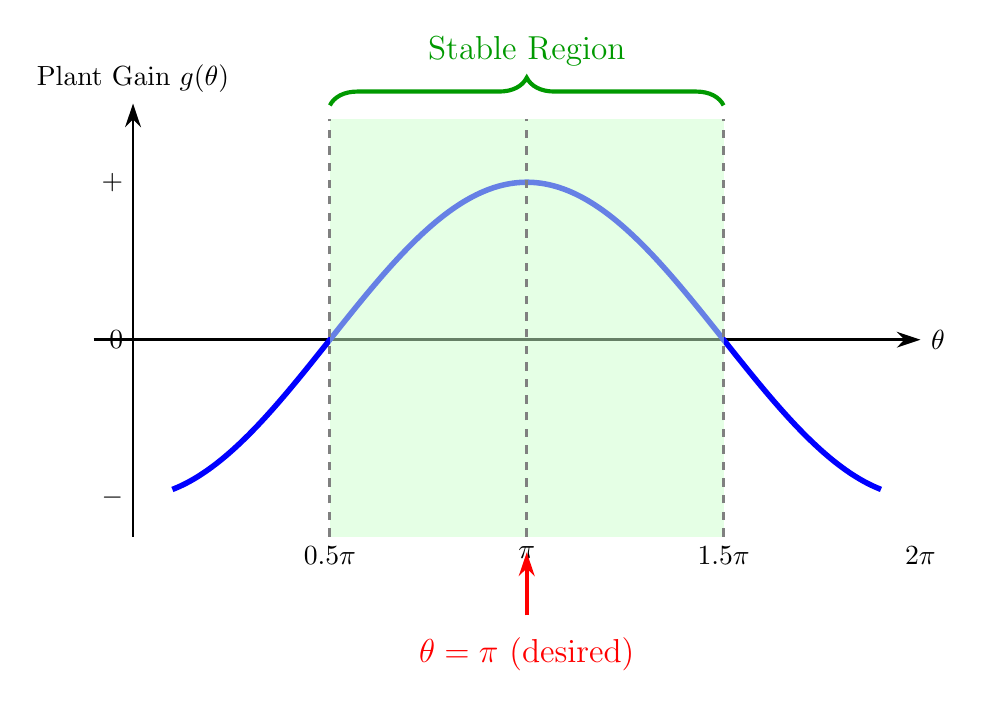
\begin{tikzpicture}[
    arrow/.style={-{Stealth[length=3mm, width=2mm]}, line width=1pt},
    label/.style={font=\large}
]
    % Axes
    \draw[arrow] (-0.5, 0) -- (10, 0) node[right] {$\theta$};
    \draw[arrow] (0, -2.5) -- (0, 3) node[above] {Plant Gain $g(\theta)$};
    
    % Labels on y-axis
    \node[left] at (0, 2) {$+$};
    \node[left] at (0, 0) {$0$};
    \node[left] at (0, -2) {$-$};
    
    % Plant gain curve (sinusoidal-like)
    \draw[line width=2pt, blue] plot[smooth, domain=0.5:9.5, samples=100] 
        (\x, {2*cos((\x-5)*36)});
    
    % Stable region shading
    \fill[green!20, opacity=0.5] (2.5, -2.5) rectangle (7.5, 2.8);
    
    % Stable region bracket
    \draw[decorate, decoration={brace, amplitude=10pt, raise=5pt}, line width=1.5pt, green!60!black]
        (2.5, 2.8) -- (7.5, 2.8) node[midway, above=15pt, font=\large, green!60!black] {Stable Region};
    
    % Vertical dashed lines
    \draw[dashed, gray, line width=1pt] (2.5, -2.5) -- (2.5, 2.8);
    \draw[dashed, gray, line width=1pt] (5, -2.5) -- (5, 2.8);
    \draw[dashed, gray, line width=1pt] (7.5, -2.5) -- (7.5, 2.8);
    
    % X-axis labels
    \node[below] at (2.5, -2.5) {$0.5\pi$};
    \node[below] at (5, -2.5) {$\pi$};
    \node[below] at (7.5, -2.5) {$1.5\pi$};
    \node[below] at (10, -2.5) {$2\pi$};
    
    % Desired operating point
    \draw[arrow, red, line width=1.5pt] (5, -3.5) -- (5, -2.7);
    \node[red, font=\large] at (5, -4) {$\theta = \pi$ (desired)};
    
\end{tikzpicture}
\caption{Plant gain $g(\theta)$ versus operating point $\theta$. The system is stable only within the shaded region.}
\end{figure}

\begin{itemize}
    \item If $|e| < 0.5\pi$: System remains stable
    \item If $|e| > 0.5\pi$: Plant gain changes sign $\rightarrow$ \textbf{Unstable!}
\end{itemize}

\subsection{Maximum Allowable Phase Error}

Using a safety margin:
\begin{equation}
|e|_{max} = 0.4\pi
\end{equation}

% =============================================================================
\section{Deriving Maximum Detectable Speed}
% =============================================================================

\subsection{From Phase Error Equation}

\begin{equation}
e_{ss} = \frac{2v\omega_n}{c \cdot \omega_{BW}} \leq 0.4\pi
\end{equation}

\subsection{Solve for Maximum Speed}

\begin{equation}
v_{max} = \frac{0.4\pi \cdot c \cdot \omega_{BW}}{2\omega_n} = \frac{\pi \omega_{BW}}{5\omega_n} \cdot c
\end{equation}

This is \textbf{equation (18)} in the paper:
\begin{equation}
\boxed{v_{max} = \frac{\pi \omega_{BW}}{5\omega_n} \cdot c \text{ (m/s)}}
\end{equation}

% =============================================================================
\section{Physical Interpretation}
% =============================================================================

\subsection{Analogy: Car Following}

% TikZ: Car Following Analogy
\begin{figure}[h]
\centering
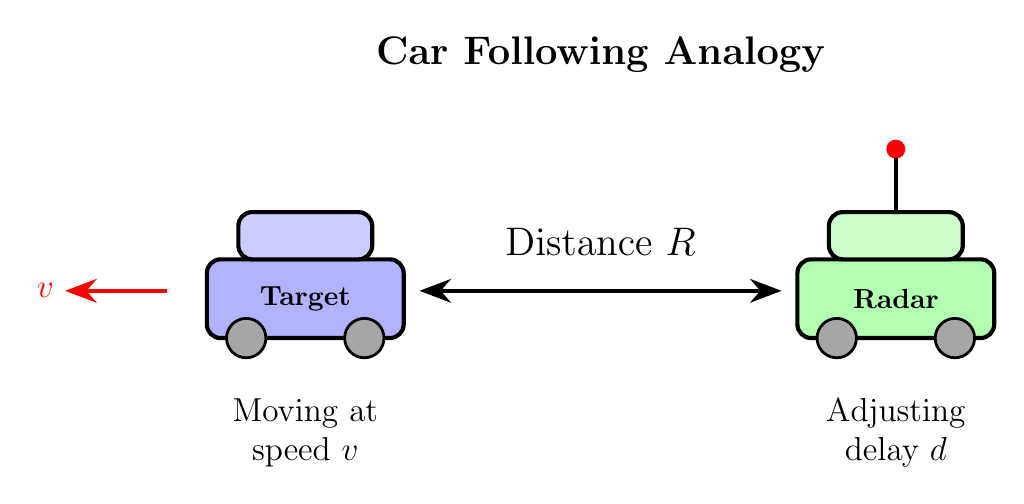
\begin{tikzpicture}[
    wheel/.style={circle, draw=black, fill=gray!70, minimum size=0.5cm, line width=1pt},
    carbody/.style={rectangle, draw=black, line width=1.5pt, rounded corners=5pt},
    arrow/.style={-{Stealth[length=4mm, width=3mm]}, line width=1.5pt},
    label/.style={font=\large}
]

    % Title
    \node[font=\Large\bfseries] at (5, 4) {Car Following Analogy};

    % === Target Car ===
    \begin{scope}[shift={(0,0)}]
        % Car body
        \draw[carbody, fill=blue!30] (0, 0.4) rectangle (2.5, 1.4);
        % Car top
        \draw[carbody, fill=blue!20] (0.4, 1.4) rectangle (2.1, 2);
        % Wheels
        \node[wheel] at (0.5, 0.4) {};
        \node[wheel] at (2.0, 0.4) {};
        % Label
        \node[font=\bfseries] at (1.25, 0.9) {Target};
    \end{scope}

    % Target label
    \node[label, align=center] at (1.25, -0.8) {Moving at\\speed $v$};

    % Velocity arrow
    \draw[arrow, red] (-0.5, 1) -- (-1.8, 1) node[left, font=\large] {$v$};

    % === Radar Car ===
    \begin{scope}[shift={(7.5,0)}]
        % Car body
        \draw[carbody, fill=green!30] (0, 0.4) rectangle (2.5, 1.4);
        % Car top
        \draw[carbody, fill=green!20] (0.4, 1.4) rectangle (2.1, 2);
        % Wheels
        \node[wheel] at (0.5, 0.4) {};
        \node[wheel] at (2.0, 0.4) {};
        % Label
        \node[font=\bfseries] at (1.25, 0.9) {Radar};
        % Antenna
        \draw[line width=1.5pt] (1.25, 2) -- (1.25, 2.8);
        \fill[red] (1.25, 2.8) circle (0.12);
    \end{scope}

    % Radar label
    \node[label, align=center] at (8.75, -0.8) {Adjusting\\delay $d$};

    % === Distance Arrow ===
    \draw[{Stealth[length=4mm, width=3mm]}-{Stealth[length=4mm, width=3mm]}, line width=1.5pt] 
        (2.7, 1) -- (7.3, 1) 
        node[midway, above=0.3cm, font=\Large] {Distance $R$};

\end{tikzpicture}
\caption{Car following analogy: The radar controller tries to ``follow'' the target by adjusting the delay $d$.}
\end{figure}

\begin{table}[h]
\centering
\renewcommand{\arraystretch}{1.5}
\begin{tabular}{ll}
\toprule
\textbf{Scenario} & \textbf{Result} \\
\midrule
Target moves slowly & Radar easily tracks \\
Target moves fast & Radar struggles to keep up \\
Target moves too fast & \textcolor{red}{Radar loses the target} \\
\bottomrule
\end{tabular}
\caption{Effect of target speed on radar tracking.}
\end{table}

\textbf{Maximum speed} = The fastest the target can move while radar still tracks it!

% =============================================================================
\section{Numerical Example}
% =============================================================================

From the paper's design:

\begin{table}[h]
\centering
\renewcommand{\arraystretch}{1.5}
\begin{tabular}{ll}
\toprule
\textbf{Parameter} & \textbf{Value} \\
\midrule
$\omega_{BW}$ & $2\pi \times 3820$ rad/s \\
$\omega_n$ & $2\pi \times 40000$ rad/s \\
$c$ & 340 m/s (sound in air) \\
\bottomrule
\end{tabular}
\caption{Design parameters from the paper.}
\end{table}

Calculation:
\begin{align}
v_{max} &= \frac{\pi \times 2\pi \times 3820}{5 \times 2\pi \times 40000} \times 340 \\
&= \frac{\pi \times 3820}{5 \times 40000} \times 340 \\
&= \frac{3.14159 \times 3820}{200000} \times 340 \\
&= \boxed{20.4 \text{ m/s}}
\end{align}

This is \textbf{much faster} than human chest movement ($\sim$0.04 m/s), so the radar works well!

% =============================================================================
\section{Speed vs Tracking Capability}
% =============================================================================

% TikZ: Speed Comparison Figure
\begin{figure}[h]
\centering
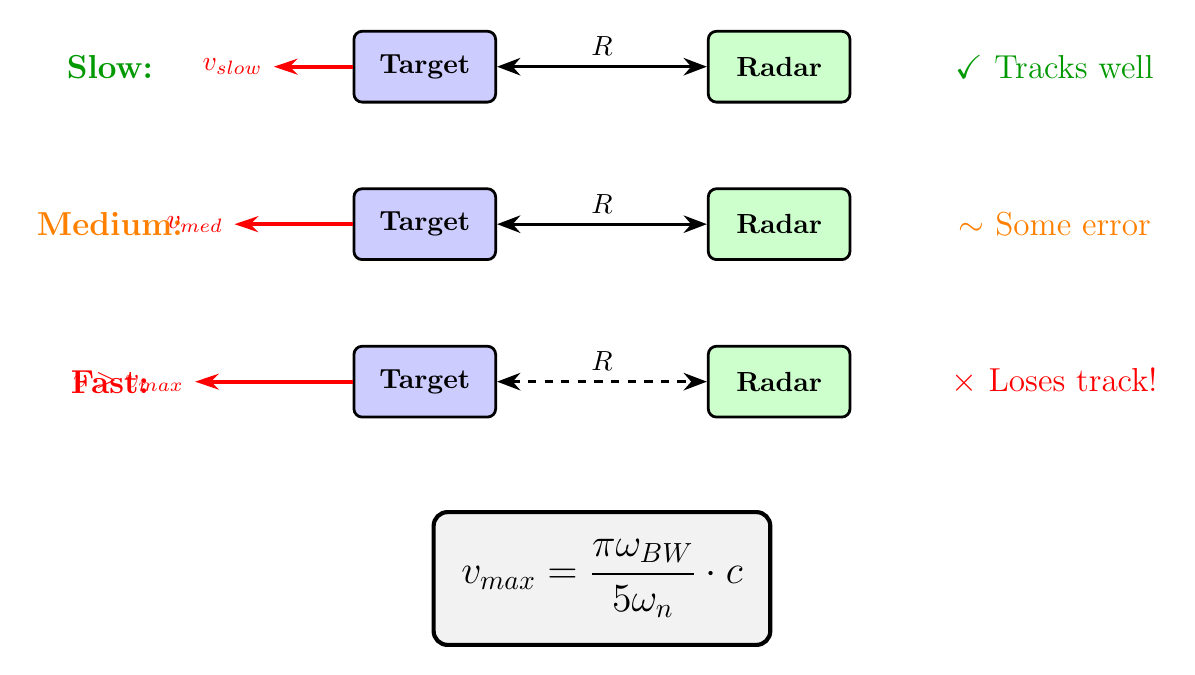
\begin{tikzpicture}[
    car/.style={rectangle, draw=black, line width=1pt, minimum width=1.8cm, 
                minimum height=0.9cm, rounded corners=3pt, font=\bfseries},
    arrow/.style={-{Stealth[length=3mm, width=2mm]}, line width=1.5pt},
    label/.style={font=\large\bfseries}
]

    % === Row 1: Slow Target ===
    \node[label, green!60!black] at (-2.5, 3) {Slow:};
    \node[car, fill=blue!20] (t1) at (1.5, 3) {Target};
    \node[car, fill=green!20] (r1) at (6, 3) {Radar};
    \draw[{Stealth}-{Stealth}, line width=1.2pt] (t1.east) -- (r1.west) 
        node[midway, above] {$R$};
    \draw[arrow, red] (t1.west) -- ++(-1, 0) node[left] {$v_{slow}$};
    \node[green!60!black, font=\large] at (9.5, 3) {$\checkmark$ Tracks well};

    % === Row 2: Medium Target ===
    \node[label, orange] at (-2.5, 1) {Medium:};
    \node[car, fill=blue!20] (t2) at (1.5, 1) {Target};
    \node[car, fill=green!20] (r2) at (6, 1) {Radar};
    \draw[{Stealth}-{Stealth}, line width=1.2pt] (t2.east) -- (r2.west) 
        node[midway, above] {$R$};
    \draw[arrow, red] (t2.west) -- ++(-1.5, 0) node[left] {$v_{med}$};
    \node[orange, font=\large] at (9.5, 1) {$\sim$ Some error};

    % === Row 3: Fast Target ===
    \node[label, red] at (-2.5, -1) {Fast:};
    \node[car, fill=blue!20] (t3) at (1.5, -1) {Target};
    \node[car, fill=green!20] (r3) at (6, -1) {Radar};
    \draw[{Stealth}-{Stealth}, line width=1.2pt, dashed] (t3.east) -- (r3.west) 
        node[midway, above] {$R$};
    \draw[arrow, red] (t3.west) -- ++(-2, 0) node[left] {$v > v_{max}$};
    \node[red, font=\large] at (9.5, -1) {$\times$ Loses track!};

    % Equation box
    \node[draw, fill=gray!10, rounded corners=5pt, line width=1.5pt, 
          font=\Large, inner sep=10pt] at (3.75, -3.5) 
        {$\displaystyle v_{max} = \frac{\pi \omega_{BW}}{5\omega_n} \cdot c$};

\end{tikzpicture}
\caption{Effect of target speed on radar tracking capability.}
\end{figure}

% =============================================================================
\section{Summary: Why Maximum Speed = Disturbance Rejection}
% =============================================================================

\begin{table}[h]
\centering
\renewcommand{\arraystretch}{1.8}
\begin{tabular}{ll}
\toprule
\textbf{Concept} & \textbf{Explanation} \\
\midrule
Disturbance & Doppler phase shift from target motion \\
Disturbance rate & Proportional to target speed $v$ \\
Controller job & Cancel phase shift by adjusting delay $d$ \\
Controller limit & Bandwidth $\omega_{BW}$ limits how fast it can respond \\
Failure mode & If target too fast $\rightarrow$ phase error too large $\rightarrow$ instability \\
Metric & $v_{max}$ = maximum speed before failure \\
\bottomrule
\end{tabular}
\caption{Summary of disturbance rejection concepts.}
\end{table}

\vspace{1cm}

% Final Key Equation Box
\begin{figure}[h]
\centering
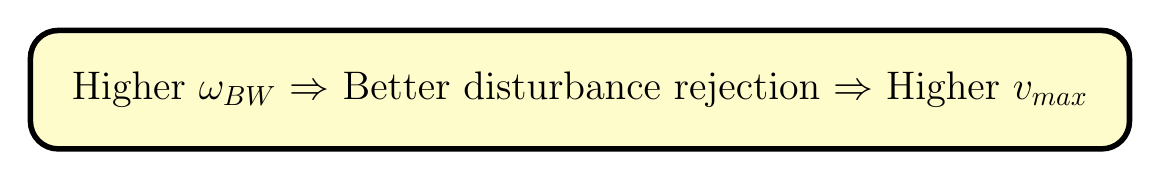
\begin{tikzpicture}
    \node[draw=black, fill=yellow!20, rounded corners=10pt, line width=2pt, 
          font=\Large, inner sep=15pt] at (0, 0) 
        {Higher $\omega_{BW}$ $\Rightarrow$ Better disturbance rejection $\Rightarrow$ Higher $v_{max}$};
\end{tikzpicture}
\end{figure}
\section{Simplified Open-Loop Transfer Function}
% =============================================================================

\textbf{Before cancellation:}
\begin{equation}
C(s)\hat{P}(s) = \frac{\omega_{BW}(s + \omega_c)}{k\omega_c \cdot s} \cdot \frac{-k\omega_c}{s + \omega_c}
\end{equation}

\textbf{After cancellation:}
\begin{equation}
C(s)\hat{P}(s) = \frac{-\omega_{BW}}{s}
\end{equation}

This is a \textbf{pure integrator} — the simplest possible open-loop system!

% TikZ: Before and After Cancellation
\begin{figure}[h]
\centering
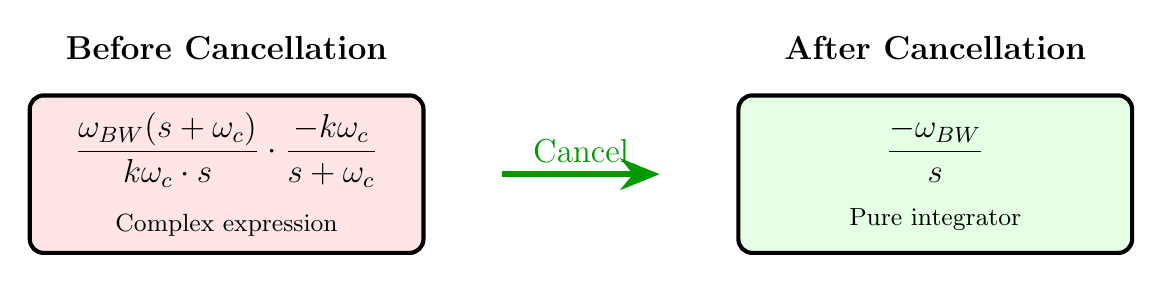
\begin{tikzpicture}[
    block/.style={rectangle, draw=black, line width=1.5pt, rounded corners=5pt,
                  minimum width=5cm, minimum height=2cm, font=\large, align=center},
    arrow/.style={-{Stealth[length=5mm, width=4mm]}, line width=2pt}
]
    % Before
    \node[block, fill=red!10] (before) at (0, 0) {
        $\displaystyle \frac{\omega_{BW}(s + \omega_c)}{k\omega_c \cdot s} \cdot \frac{-k\omega_c}{s + \omega_c}$\\[0.3cm]
        \small Complex expression
    };
    \node[font=\large\bfseries, above=0.3cm of before] {Before Cancellation};
    
    % Arrow
    \draw[arrow, green!60!black] (3.5, 0) -- (5.5, 0) node[midway, above, font=\large] {Cancel};
    
    % After
    \node[block, fill=green!10] (after) at (9, 0) {
        $\displaystyle \frac{-\omega_{BW}}{s}$\\[0.3cm]
        \small Pure integrator
    };
    \node[font=\large\bfseries, above=0.3cm of after] {After Cancellation};
    
\end{tikzpicture}
\caption{Simplification of open-loop transfer function through pole-zero cancellation.}
\end{figure}

% =============================================================================
\section{Predictable Closed-Loop Behavior}
% =============================================================================

The closed-loop transfer function becomes:
\begin{equation}
T(s) = \frac{C(s)\hat{P}(s)}{1 + C(s)\hat{P}(s)} = \frac{-\omega_{BW}/s}{1 + (-\omega_{BW}/s)} = \frac{-\omega_{BW}}{s - \omega_{BW}}
\end{equation}

This is a \textbf{first-order system} with:
\begin{itemize}
    \item Time constant: $\tau = \dfrac{1}{\omega_{BW}}$
    \item Bandwidth: $\omega_{BW}$
    \item No overshoot
    \item No oscillations
\end{itemize}

% =============================================================================
\section{Single Design Parameter}
% =============================================================================

\begin{table}[h]
\centering
\renewcommand{\arraystretch}{1.8}
\begin{tabular}{ll}
\toprule
\textbf{Without Cancellation} & \textbf{With Cancellation} \\
\midrule
Multiple parameters to tune & Only \textbf{one} parameter: $\omega_{BW}$ \\
Complex trade-offs & Simple trade-off \\
Difficult optimization & Easy optimization \\
\bottomrule
\end{tabular}
\caption{Comparison of design complexity.}
\end{table}

\textbf{Design becomes trivial:}
\begin{itemize}
    \item Want faster response? $\rightarrow$ Increase $\omega_{BW}$
    \item Want more stability? $\rightarrow$ Decrease $\omega_{BW}$
\end{itemize}

% TikZ: Single Parameter Design
\begin{figure}[h]
\centering
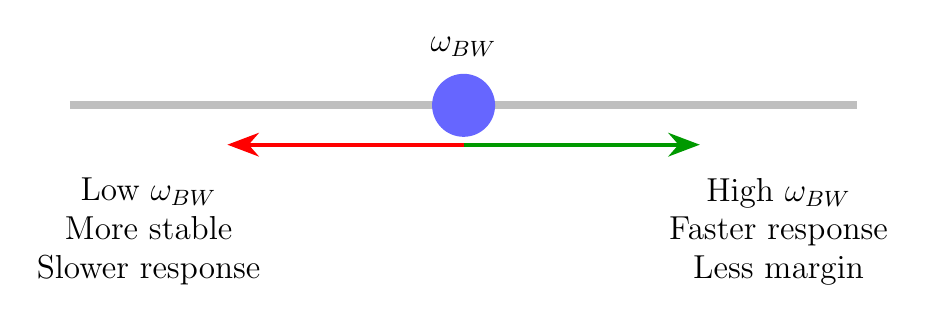
\begin{tikzpicture}[
    arrow/.style={-{Stealth[length=4mm, width=3mm]}, line width=1.5pt}
]
    % Slider bar
    \draw[line width=3pt, gray!50] (0, 0) -- (10, 0);
    
    % Slider knob
    \fill[blue!60] (5, 0) circle (0.4);
    \node[above=0.5cm, font=\large\bfseries] at (5, 0) {$\omega_{BW}$};
    
    % Labels
    \node[below=0.8cm, font=\large, align=center] at (1, 0) {Low $\omega_{BW}$\\More stable\\Slower response};
    \node[below=0.8cm, font=\large, align=center] at (9, 0) {High $\omega_{BW}$\\Faster response\\Less margin};
    
    % Arrows
    \draw[arrow, red] (5, -0.5) -- (2, -0.5);
    \draw[arrow, green!60!black] (5, -0.5) -- (8, -0.5);
    
\end{tikzpicture}
\caption{Single design parameter $\omega_{BW}$ controls the trade-off between speed and stability.}
\end{figure}

% =============================================================================
\section{Guaranteed Stability Margins}
% =============================================================================

For pure integrator $\dfrac{-\omega_{BW}}{s}$:

\begin{table}[h]
\centering
\renewcommand{\arraystretch}{1.8}
\begin{tabular}{lcc}
\toprule
\textbf{Stability Metric} & \textbf{Value} & \textbf{Quality} \\
\midrule
Phase Margin & $90°$ & Excellent \\
Gain Margin & $\infty$ & Excellent \\
Crossover Frequency & $\omega_{BW}$ & Controllable \\
\bottomrule
\end{tabular}
\caption{Stability margins for pure integrator.}
\end{table}

% TikZ: Bode Plot of Pure Integrator
\begin{figure}[h]
\centering
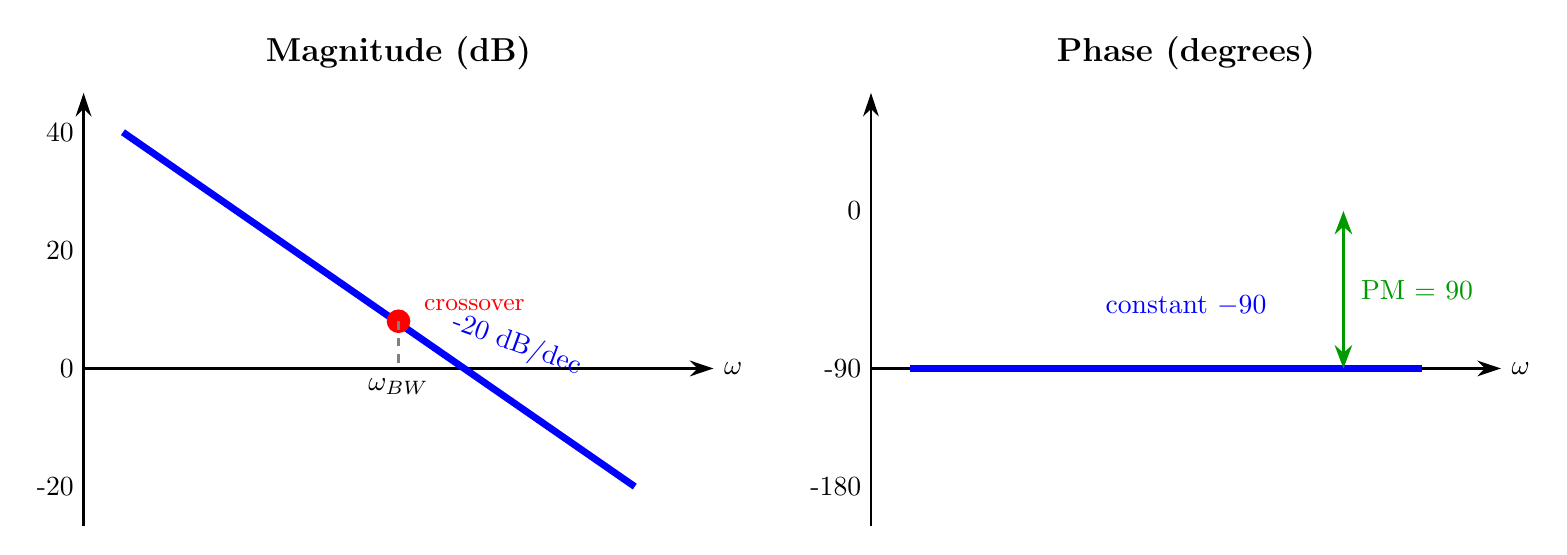
\begin{tikzpicture}[
    arrow/.style={-{Stealth[length=3mm, width=2mm]}, line width=1pt}
]
    % === Magnitude Plot ===
    \begin{scope}[shift={(0, 0)}]
        % Title
        \node[font=\large\bfseries] at (4, 4) {Magnitude (dB)};
        
        % Axes
        \draw[arrow] (0, 0) -- (8, 0) node[right] {$\omega$};
        \draw[arrow] (0, -2) -- (0, 3.5);
        
        % Y-axis labels
        \node[left] at (0, 3) {40};
        \node[left] at (0, 1.5) {20};
        \node[left] at (0, 0) {0};
        \node[left] at (0, -1.5) {-20};
        
        % Magnitude line (-20 dB/decade slope)
        \draw[line width=2.5pt, blue] (0.5, 3) -- (7, -1.5);
        
        % Crossover point
        \fill[red] (4, 0.6) circle (0.15);
        \draw[dashed, gray, line width=1pt] (4, 0.6) -- (4, 0);
        \node[below, font=\normalsize] at (4, 0) {$\omega_{BW}$};
        \node[right, font=\small, red] at (4.2, 0.8) {crossover};
        
        % Slope annotation
        \node[font=\normalsize, blue, rotate=-20] at (5.5, 0.3) {-20 dB/dec};
    \end{scope}
    
    % === Phase Plot ===
    \begin{scope}[shift={(10, 0)}]
        % Title
        \node[font=\large\bfseries] at (4, 4) {Phase (degrees)};
        
        % Axes
        \draw[arrow] (0, 0) -- (8, 0) node[right] {$\omega$};
        \draw[arrow] (0, -2) -- (0, 3.5);
        
        % Y-axis labels
        \node[left] at (0, 2) {0};
        \node[left] at (0, 0) {-90};
        \node[left] at (0, -1.5) {-180};
        
        % Phase line (constant -90°)
        \draw[line width=2.5pt, blue] (0.5, 0) -- (7, 0);
        
        % Annotation
        \node[font=\normalsize, blue] at (4, 0.8) {constant $-90°$};
        
        % Phase margin annotation
        \draw[{Stealth}-{Stealth}, line width=1.2pt, green!60!black] (6, 0) -- (6, 2);
        \node[right, font=\normalsize, green!60!black] at (6.1, 1) {PM = $90°$};
    \end{scope}
    
\end{tikzpicture}
\caption{Bode plot of pure integrator $\frac{-\omega_{BW}}{s}$.}
\end{figure}

% =============================================================================
\section{Perfect Disturbance Rejection (at DC)}
% =============================================================================

The integrator provides \textbf{infinite gain at DC} ($s = 0$):
\begin{equation}
|C(0)\hat{P}(0)| = \left|\frac{-\omega_{BW}}{0}\right| = \infty
\end{equation}

This means:
\begin{itemize}
    \item \textbf{Zero steady-state error} for step disturbances
    \item \textbf{Perfect tracking} of constant references
    \item Doppler phase shift is \textbf{completely cancelled}
\end{itemize}

% =============================================================================
\section{Decoupled Design}
% =============================================================================

% TikZ: Decoupled Design Comparison
\begin{figure}[h]
\centering
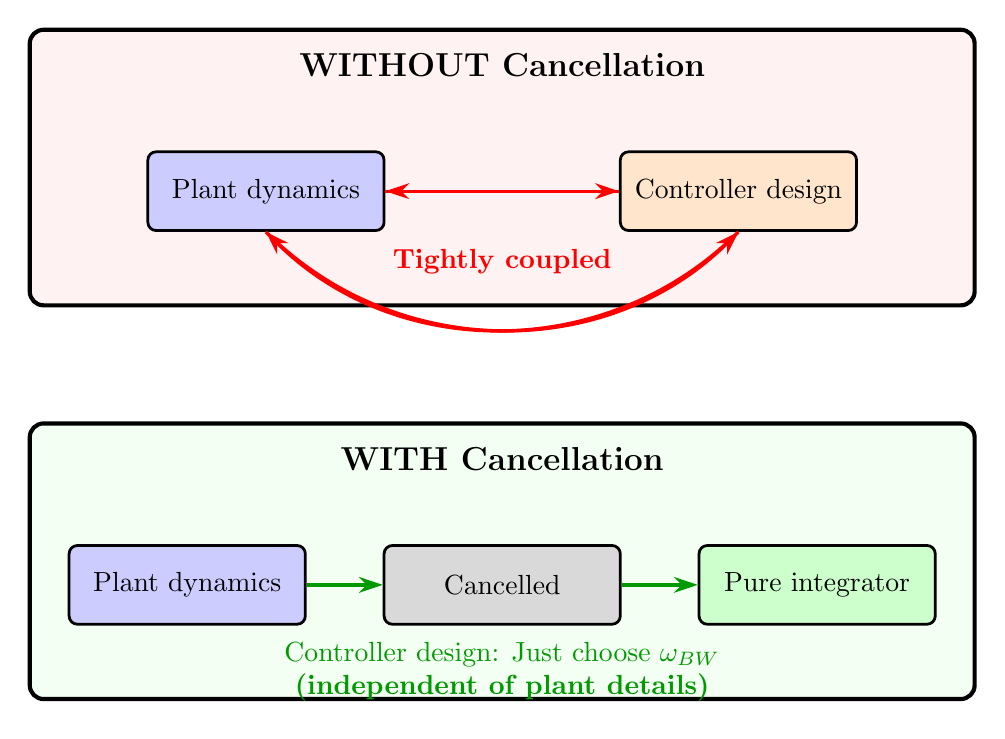
\begin{tikzpicture}[
    box/.style={rectangle, draw=black, line width=1.5pt, rounded corners=5pt,
                minimum width=12cm, minimum height=3.5cm},
    innerbox/.style={rectangle, draw=black, line width=1pt, rounded corners=3pt,
                     minimum width=3cm, minimum height=1cm, font=\normalsize},
    arrow/.style={-{Stealth[length=3mm, width=2mm]}, line width=1.2pt}
]
    % === WITHOUT Cancellation ===
    \begin{scope}[shift={(0, 4)}]
        % Main box
        \node[box, fill=red!5] (without) at (0, 0) {};
        \node[font=\large\bfseries] at (0, 1.3) {WITHOUT Cancellation};
        
        % Inner elements
        \node[innerbox, fill=blue!20] (plant1) at (-3, -0.3) {Plant dynamics};
        \node[innerbox, fill=orange!20] (ctrl1) at (3, -0.3) {Controller design};
        
        % Bidirectional coupling
        \draw[arrow, red] (plant1.east) -- (ctrl1.west);
        \draw[arrow, red] (ctrl1.west) -- (plant1.east);
        \draw[arrow, red] (plant1.south) to[out=-45, in=-135] (ctrl1.south);
        \draw[arrow, red] (ctrl1.south) to[out=-135, in=-45] (plant1.south);
        
        % Label
        \node[font=\normalsize, red] at (0, -1.2) {\textbf{Tightly coupled}};
    \end{scope}
    
    % === WITH Cancellation ===
    \begin{scope}[shift={(0, -1)}]
        % Main box
        \node[box, fill=green!5] (with) at (0, 0) {};
        \node[font=\large\bfseries] at (0, 1.3) {WITH Cancellation};
        
        % Inner elements
        \node[innerbox, fill=blue!20] (plant2) at (-4, -0.3) {Plant dynamics};
        \node[innerbox, fill=gray!30] (cancel) at (0, -0.3) {Cancelled};
        \node[innerbox, fill=green!20] (integ) at (4, -0.3) {Pure integrator};
        
        % Arrows
        \draw[arrow, green!60!black] (plant2.east) -- (cancel.west);
        \draw[arrow, green!60!black] (cancel.east) -- (integ.west);
        
        % Label
        \node[font=\normalsize, green!60!black, align=center] at (0, -1.4) {
            Controller design: Just choose $\omega_{BW}$\\
            \textbf{(independent of plant details)}
        };
    \end{scope}
    
\end{tikzpicture}
\caption{Comparison of design coupling with and without pole-zero cancellation.}
\end{figure}

% =============================================================================
\section{Robustness to Plant Variations}
% =============================================================================

Even if the plant parameters change slightly:

\begin{table}[h]
\centering
\renewcommand{\arraystretch}{1.8}
\begin{tabular}{ll}
\toprule
\textbf{Scenario} & \textbf{Effect} \\
\midrule
Perfect cancellation & Ideal integrator response \\
Imperfect cancellation & Small residual pole, still stable \\
Large mismatch & May need to retune $\omega_{BW}$ \\
\bottomrule
\end{tabular}
\caption{Effect of plant variations on system performance.}
\end{table}

The cancelled pole is \textbf{stable} ($s = -\omega_c < 0$), so even imperfect cancellation doesn't cause instability.

% =============================================================================
\section{Comparison: With vs Without Pole-Zero Cancellation}
% =============================================================================

\begin{table}[h]
\centering
\renewcommand{\arraystretch}{1.8}
\begin{tabular}{lcc}
\toprule
\textbf{Aspect} & \textbf{Without Cancellation} & \textbf{With Cancellation} \\
\midrule
Open-loop order & Higher order & 1st order (integrator) \\
Design parameters & Multiple ($k_p$, $k_I$, ...) & Single ($\omega_{BW}$) \\
Phase margin & Varies, needs calculation & $90°$ (guaranteed) \\
Gain margin & Varies, needs calculation & $\infty$ (guaranteed) \\
Steady-state error & May be non-zero & Zero \\
Step response & May have overshoot & No overshoot \\
Tuning complexity & High & Low \\
Closed-loop poles & Multiple & Single pole at $-\omega_{BW}$ \\
\bottomrule
\end{tabular}
\caption{Comprehensive comparison of control system characteristics.}
\end{table}

% =============================================================================
\section{Graphical Comparison}
% =============================================================================

\subsection{Step Response}

% TikZ: Step Response Comparison
\begin{figure}[h]
\centering
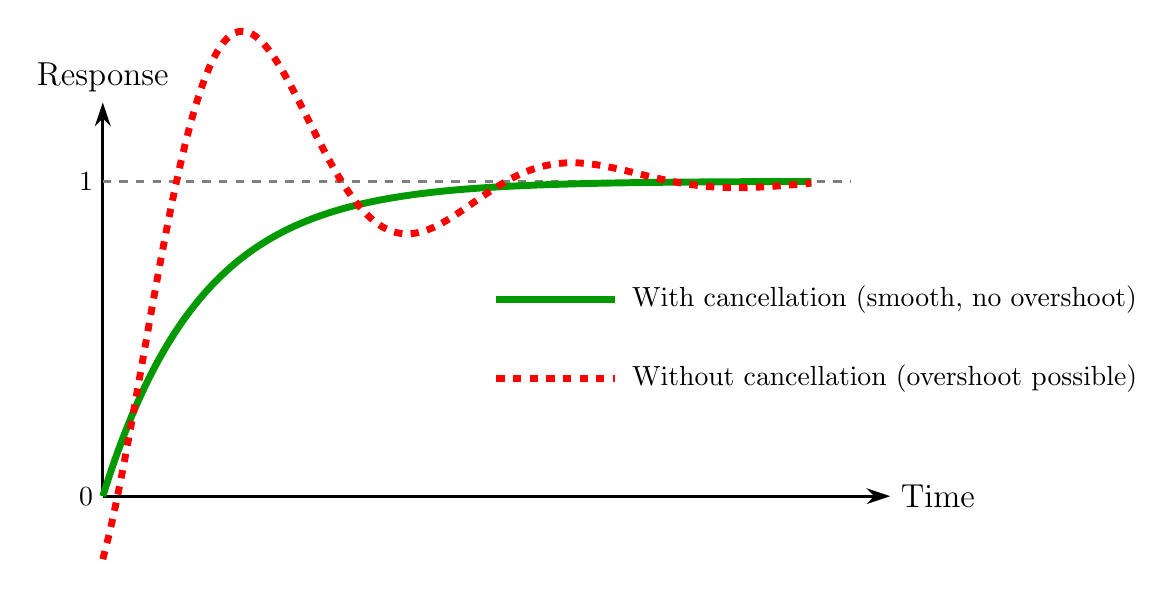
\begin{tikzpicture}[
    arrow/.style={-{Stealth[length=3mm, width=2mm]}, line width=1pt}
]
    % Axes
    \draw[arrow] (0, 0) -- (10, 0) node[right, font=\large] {Time};
    \draw[arrow] (0, 0) -- (0, 5) node[above, font=\large] {Response};
    
    % Y-axis labels
    \node[left] at (0, 4) {1};
    \node[left] at (0, 0) {0};
    
    % Reference line
    \draw[dashed, gray, line width=1pt] (0, 4) -- (9.5, 4);
    
    % WITH cancellation (smooth, no overshoot)
    \draw[line width=2.5pt, green!60!black] plot[smooth, domain=0:9, samples=100] 
        (\x, {4*(1 - exp(-0.8*\x))});
    
    % WITHOUT cancellation (overshoot)
    \draw[line width=2.5pt, red, dashed] plot[smooth, domain=0:9, samples=100] 
        (\x, {4*(1 - 1.2*exp(-0.5*\x)*cos(deg(1.5*\x)) + 0.2*exp(-0.5*\x)*sin(deg(1.5*\x)))});
    
    % Legend
    \draw[line width=2.5pt, green!60!black] (5, 2.5) -- (6.5, 2.5);
    \node[right, font=\normalsize] at (6.6, 2.5) {With cancellation (smooth, no overshoot)};
    
    \draw[line width=2.5pt, red, dashed] (5, 1.5) -- (6.5, 1.5);
    \node[right, font=\normalsize] at (6.6, 1.5) {Without cancellation (overshoot possible)};
    
\end{tikzpicture}
\caption{Step response comparison: with vs without pole-zero cancellation.}
\end{figure}

\subsection{Bode Plot (Open-Loop)}

% TikZ: Bode Plot Comparison
\begin{figure}[h]
\centering
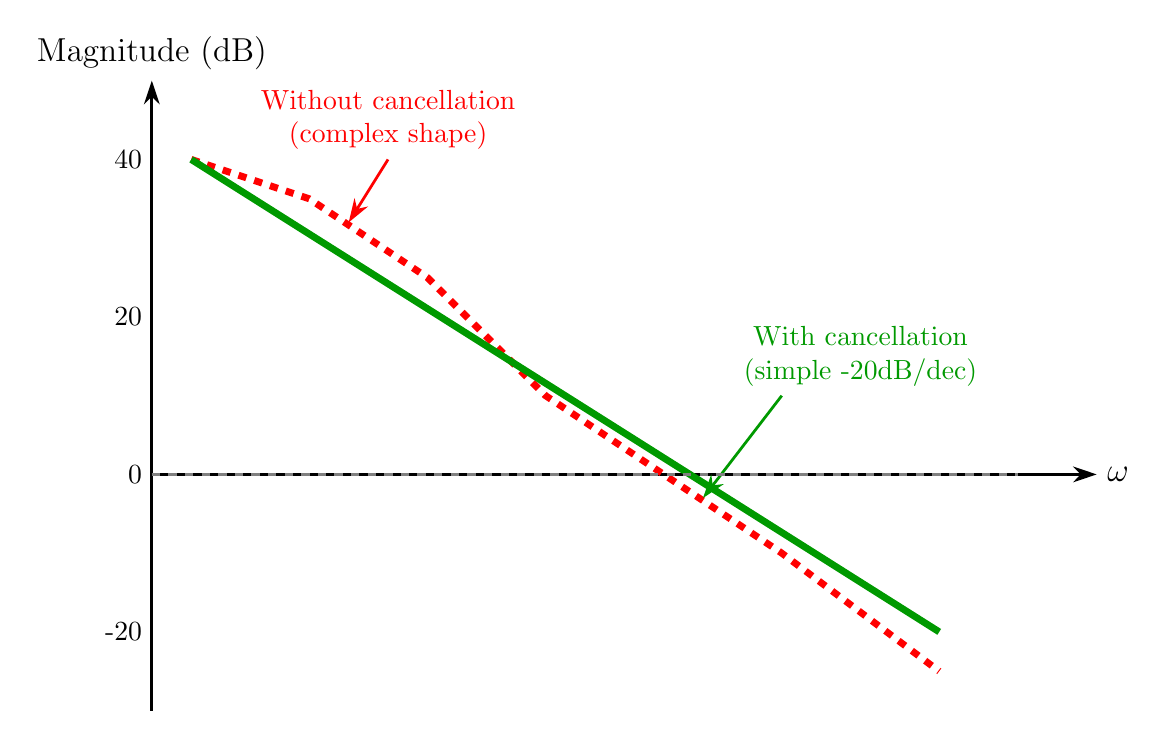
\begin{tikzpicture}[
    arrow/.style={-{Stealth[length=3mm, width=2mm]}, line width=1pt}
]
    % Axes
    \draw[arrow] (0, 0) -- (12, 0) node[right, font=\large] {$\omega$};
    \draw[arrow] (0, -3) -- (0, 5) node[above, font=\large] {Magnitude (dB)};
    
    % Y-axis labels
    \node[left] at (0, 4) {40};
    \node[left] at (0, 2) {20};
    \node[left] at (0, 0) {0};
    \node[left] at (0, -2) {-20};
    
    % WITHOUT cancellation (complex shape)
    \draw[line width=2.5pt, red, dashed] 
        (0.5, 4) -- (2, 3.5) -- (3.5, 2.5) -- (5, 1) -- (6.5, 0) -- (8, -1) -- (10, -2.5);
    
    % WITH cancellation (simple -20dB/dec)
    \draw[line width=2.5pt, green!60!black] 
        (0.5, 4) -- (10, -2);
    
    % Annotations
    \node[font=\normalsize, red, align=center] at (3, 4.5) {Without cancellation\\(complex shape)};
    \draw[arrow, red] (3, 4) -- (2.5, 3.2);
    
    \node[font=\normalsize, green!60!black, align=center] at (9, 1.5) {With cancellation\\(simple -20dB/dec)};
    \draw[arrow, green!60!black] (8, 1) -- (7, -0.3);
    
    % 0 dB crossing
    \draw[dashed, gray, line width=1pt] (0, 0) -- (11, 0);
    
\end{tikzpicture}
\caption{Open-loop Bode plot comparison: with vs without pole-zero cancellation.}
\end{figure}

% =============================================================================
\section{Mathematical Proof of Benefits}
% =============================================================================

\subsection{Benefit 1: Zero Steady-State Error}

For a step disturbance $D(s) = \frac{1}{s}$, the steady-state error is:

\begin{align}
e_{ss} &= \lim_{s \to 0} \frac{s \cdot D(s)}{1 + C(s)\hat{P}(s)} \\
&= \lim_{s \to 0} \frac{s \cdot \frac{1}{s}}{1 + \frac{-\omega_{BW}}{s}} \\
&= \lim_{s \to 0} \frac{1}{\frac{s - \omega_{BW}}{s}} \\
&= \lim_{s \to 0} \frac{s}{s - \omega_{BW}} \\
&= \boxed{0}
\end{align}

\subsection{Benefit 2: First-Order Closed-Loop}

\begin{equation}
T(s) = \frac{-\omega_{BW}/s}{1 - \omega_{BW}/s} = \frac{-\omega_{BW}}{s - \omega_{BW}}
\end{equation}

Step response:
\begin{equation}
y(t) = 1 - e^{-\omega_{BW} t} \quad \text{(for stable system)}
\end{equation}

With negative feedback, the system is stable with pole at $s = -\omega_{BW}$.

\begin{equation}
T(s) = \frac{L(s)}{1 + L(s)} \quad \text{where } L(s) = -\frac{\omega_{BW}}{s}
\end{equation}

% =============================================================================
\section{Summary}
% =============================================================================

% TikZ: Summary Box
\begin{figure}[h]
\centering
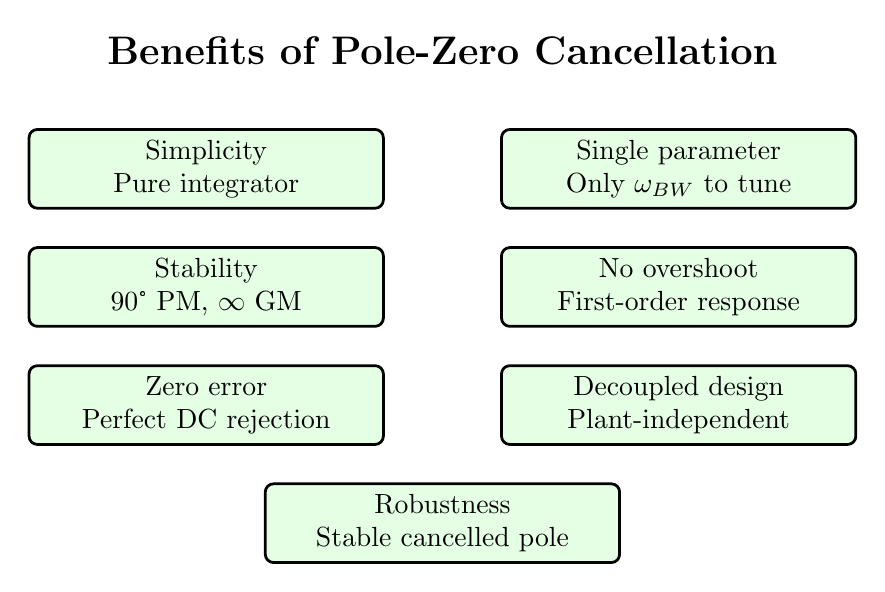
\begin{tikzpicture}[
    benefit/.style={rectangle, draw=black, line width=1pt, rounded corners=3pt,
                    minimum width=4.5cm, minimum height=1cm, font=\normalsize, 
                    fill=green!10, align=center}
]
    % Title
    \node[font=\Large\bfseries] at (5, 5) {Benefits of Pole-Zero Cancellation};
    
    % Benefits grid
    \node[benefit] at (2, 3.5) {Simplicity\\Pure integrator};
    \node[benefit] at (8, 3.5) {Single parameter\\Only $\omega_{BW}$ to tune};
    
    \node[benefit] at (2, 2) {Stability\\90° PM, $\infty$ GM};
    \node[benefit] at (8, 2) {No overshoot\\First-order response};
    
    \node[benefit] at (2, 0.5) {Zero error\\Perfect DC rejection};
    \node[benefit] at (8, 0.5) {Decoupled design\\Plant-independent};
    
    \node[benefit] at (5, -1) {Robustness\\Stable cancelled pole};
    
\end{tikzpicture}
\caption{Summary of pole-zero cancellation benefits.}
\end{figure}

\vspace{0.5cm}

% Final Key Message
\begin{figure}[h]
\centering
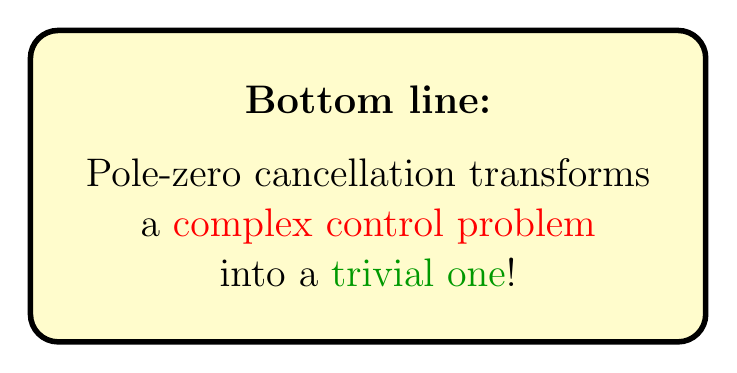
\begin{tikzpicture}
    \node[draw=black, fill=yellow!20, rounded corners=10pt, line width=2pt, 
          font=\Large, inner sep=20pt, align=center] at (0, 0) {
        \textbf{Bottom line:}\\[0.3cm]
        Pole-zero cancellation transforms\\
        a \textcolor{red}{complex control problem}\\
        into a \textcolor{green!60!black}{trivial one}!
    };
\end{tikzpicture}
\end{figure}
\section{Gain Margin and Phase Margin}

\subsection{Definitions}

\begin{table}[h]
\centering
\renewcommand{\arraystretch}{1.8}
\begin{tabular}{lll}
\toprule
\textbf{Margin} & \textbf{Definition} & \textbf{Measured At} \\
\midrule
Phase Margin (PM) & Extra phase lag before instability & Gain crossover: $|L(j\omega)| = 1$ \\
Gain Margin (GM) & Extra gain before instability & Phase crossover: $\angle L(j\omega) = -180°$ \\
\bottomrule
\end{tabular}
\caption{Definitions of stability margins.}
\end{table}

\subsection{Bode Plot Interpretation}

\begin{figure}[h]
\centering
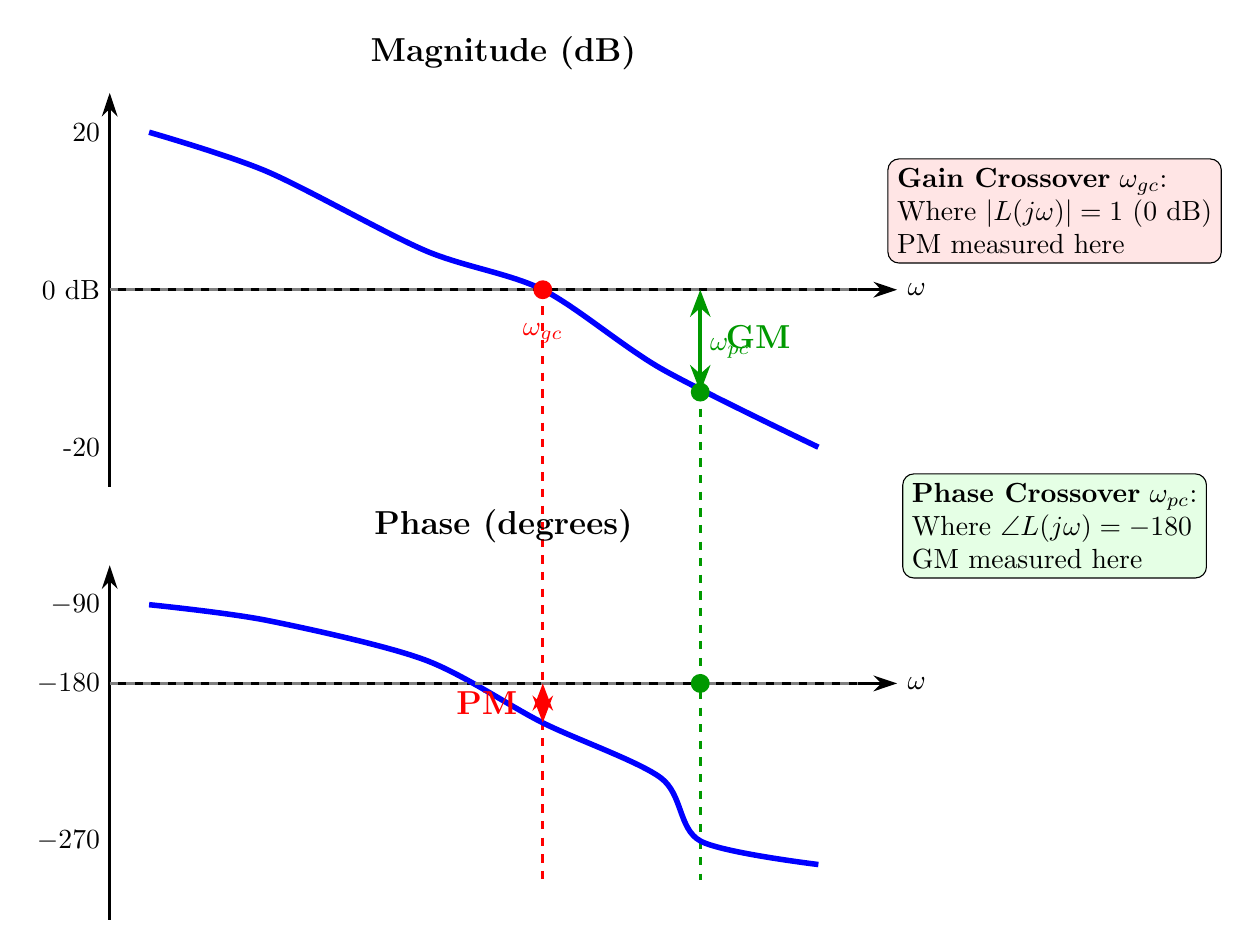
\begin{tikzpicture}[
    arrow/.style={-{Stealth[length=3mm, width=2mm]}, line width=1pt},
    label/.style={font=\normalsize}
]
    % === Magnitude Plot ===
    \begin{scope}[shift={(0, 5)}]
        % Title
        \node[font=\large\bfseries] at (5, 3) {Magnitude (dB)};
        
        % Axes
        \draw[arrow] (0, 0) -- (10, 0) node[right] {$\omega$};
        \draw[arrow] (0, -2.5) -- (0, 2.5);
        
        % Y-axis labels
        \node[left] at (0, 2) {20};
        \node[left] at (0, 0) {0 dB};
        \node[left] at (0, -2) {-20};
        
        % Magnitude curve
        \draw[line width=2pt, blue] plot[smooth] coordinates {(0.5, 2) (2, 1.5) (4, 0.5) (5.5, 0) (7, -1) (9, -2)};
        
        % 0 dB line
        \draw[dashed, gray, line width=1pt] (0, 0) -- (9.5, 0);
        
        % Gain crossover point
        \fill[red] (5.5, 0) circle (0.12);
        \node[below, red, font=\normalsize] at (5.5, -0.3) {$\omega_{gc}$};
        \draw[dashed, red, line width=1pt] (5.5, 0) -- (5.5, -7.5);
        
        % Phase crossover frequency marker
        \fill[green!60!black] (7.5, -1.3) circle (0.12);
        \node[above right, green!60!black, font=\normalsize] at (7.5, -1) {$\omega_{pc}$};
        \draw[dashed, green!60!black, line width=1pt] (7.5, -1.3) -- (7.5, -7.5);
        
        % GM arrow
        \draw[{Stealth}-{Stealth}, line width=1.5pt, green!60!black] (7.5, -1.3) -- (7.5, 0);
        \node[right, green!60!black, font=\large] at (7.7, -0.6) {\textbf{GM}};
        
    \end{scope}
    
    % === Phase Plot ===
    \begin{scope}[shift={(0, 0)}]
        % Title
        \node[font=\large\bfseries] at (5, 2) {Phase (degrees)};
        
        % Axes
        \draw[arrow] (0, 0) -- (10, 0) node[right] {$\omega$};
        \draw[arrow] (0, -3) -- (0, 1.5);
        
        % Y-axis labels
        \node[left] at (0, 1) {$-90°$};
        \node[left] at (0, 0) {$-180°$};
        \node[left] at (0, -2) {$-270°$};
        
        % Phase curve
        \draw[line width=2pt, blue] plot[smooth] coordinates {(0.5, 1) (2, 0.8) (4, 0.3) (5.5, -0.5) (7, -1.2) (7.5, -2) (9, -2.3)};
        
        % -180° line
        \draw[dashed, gray, line width=1pt] (0, 0) -- (9.5, 0);
        
        % PM measurement at gain crossover
        \draw[{Stealth}-{Stealth}, line width=1.5pt, red] (5.5, -0.5) -- (5.5, 0);
        \node[left, red, font=\large] at (5.3, -0.25) {\textbf{PM}};
        
        % Phase crossover point
        \fill[green!60!black] (7.5, 0) circle (0.12);
        
    \end{scope}
    
    % === Annotations ===
    \node[draw, fill=red!10, rounded corners, font=\normalsize, align=left] at (12, 6) {
        \textbf{Gain Crossover} $\omega_{gc}$:\\
        Where $|L(j\omega)| = 1$ (0 dB)\\
        PM measured here
    };
    
    \node[draw, fill=green!10, rounded corners, font=\normalsize, align=left] at (12, 2) {
        \textbf{Phase Crossover} $\omega_{pc}$:\\
        Where $\angle L(j\omega) = -180°$\\
        GM measured here
    };
    
\end{tikzpicture}
\caption{Gain Margin and Phase Margin on Bode plot.}
\end{figure}

\subsection{Mathematical Definitions}

\textbf{Phase Margin (PM):}
\begin{equation}
\text{PM} = 180° + \angle L(j\omega_{gc})
\end{equation}
where $\omega_{gc}$ is the \textbf{gain crossover frequency}: $|L(j\omega_{gc})| = 1$

\textbf{Gain Margin (GM):}
\begin{equation}
\text{GM} = \frac{1}{|L(j\omega_{pc})|}
\end{equation}
where $\omega_{pc}$ is the \textbf{phase crossover frequency}: $\angle L(j\omega_{pc}) = -180°$

In decibels:
\begin{equation}
\text{GM (dB)} = -20\log_{10}|L(j\omega_{pc})| = 20\log_{10}\left(\frac{1}{|L(j\omega_{pc})|}\right)
\end{equation}

\section{How Stability Depends on GM and PM}

\subsection{Stability Conditions}

\begin{table}[h]
\centering
\renewcommand{\arraystretch}{1.8}
\begin{tabular}{lccc}
\toprule
\textbf{Condition} & \textbf{GM} & \textbf{PM} & \textbf{Stability} \\
\midrule
Stable & $> 1$ (or $> 0$ dB) & $> 0°$ & $\checkmark$ Stable \\
Marginally Stable & $= 1$ (or $= 0$ dB) & $= 0°$ & On the edge \\
Unstable & $< 1$ (or $< 0$ dB) & $< 0°$ & $\times$ Unstable \\
\bottomrule
\end{tabular}
\caption{Relationship between margins and stability.}
\end{table}

\subsection{Typical Design Requirements}

\begin{table}[h]
\centering
\renewcommand{\arraystretch}{1.8}
\begin{tabular}{lcc}
\toprule
\textbf{Application} & \textbf{Minimum PM} & \textbf{Minimum GM} \\
\midrule
General control systems & $45°$ & 6 dB (factor of 2) \\
Robust systems & $60°$ & 10 dB (factor of 3) \\
High-performance systems & $30°-45°$ & 4-6 dB \\
\bottomrule
\end{tabular}
\caption{Typical design specifications for stability margins.}
\end{table}

\subsection{Effect on System Response}

\begin{figure}[h]
\centering
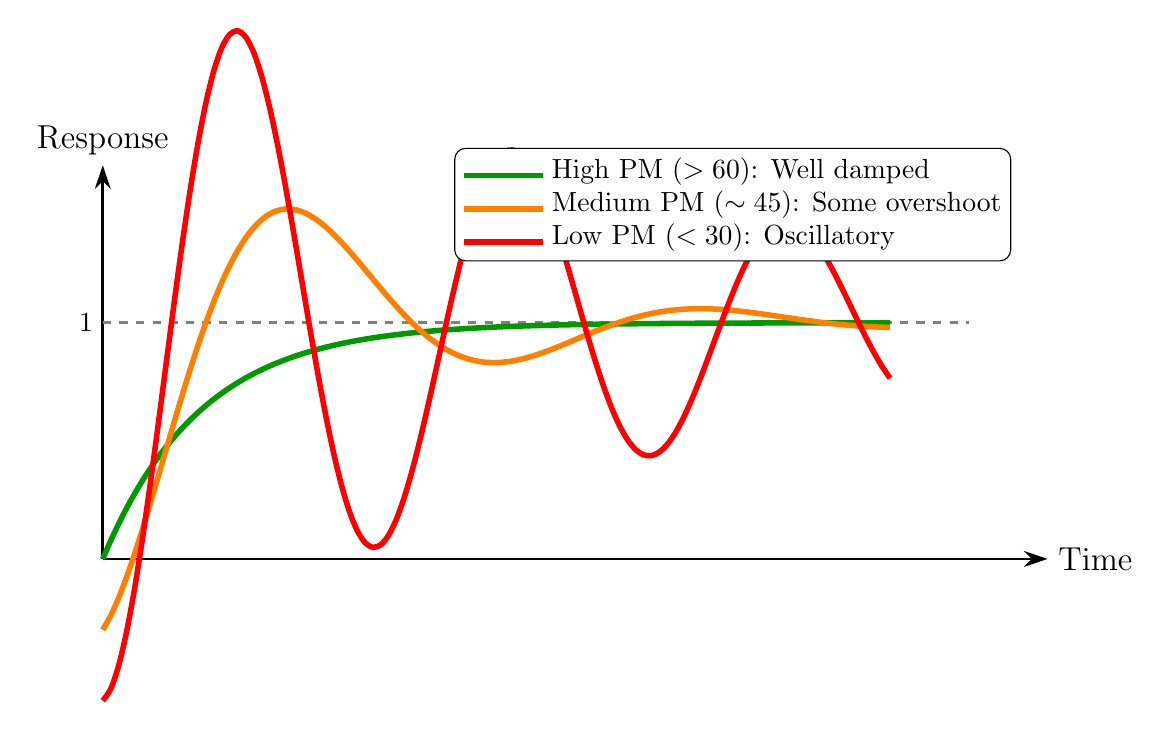
\begin{tikzpicture}[
    arrow/.style={-{Stealth[length=3mm, width=2mm]}, line width=1pt}
]
    % === Step Response Plot ===
    % Axes
    \draw[arrow] (0, 0) -- (12, 0) node[right, font=\large] {Time};
    \draw[arrow] (0, 0) -- (0, 5) node[above, font=\large] {Response};
    
    % Reference line
    \draw[dashed, gray, line width=1pt] (0, 3) -- (11, 3);
    \node[left] at (0, 3) {1};
    
    % High PM (well damped)
    \draw[line width=2pt, green!60!black] plot[smooth, domain=0:10, samples=100] 
        (\x, {3*(1 - exp(-0.8*\x))});
    
    % Medium PM (some overshoot)
    \draw[line width=2pt, orange] plot[smooth, domain=0:10, samples=100] 
        (\x, {3*(1 - 1.3*exp(-0.4*\x)*cos(deg(1.2*\x)))});
    
    % Low PM (oscillatory)
    \draw[line width=2pt, red] plot[smooth, domain=0:10, samples=100] 
        (\x, {3*(1 - 1.6*exp(-0.15*\x)*cos(deg(1.8*\x)))});
    
    % Legend
    \node[draw, fill=white, rounded corners, align=left, font=\normalsize] at (8, 4.5) {
        \textcolor{green!60!black}{\rule{1cm}{2pt}} High PM ($>60°$): Well damped\\
        \textcolor{orange}{\rule{1cm}{2pt}} Medium PM ($\sim45°$): Some overshoot\\
        \textcolor{red}{\rule{1cm}{2pt}} Low PM ($<30°$): Oscillatory
    };
    
\end{tikzpicture}
\caption{Effect of phase margin on step response.}
\end{figure}

\section{How to Calculate GM and PM}

\subsection{Method 1: Analytical Calculation}

Given open-loop transfer function $L(s)$:

\textbf{Step 1: Find Gain Crossover Frequency $\omega_{gc}$}

Solve for $\omega$ where magnitude equals 1:
\begin{equation}
|L(j\omega_{gc})| = 1
\end{equation}

\textbf{Step 2: Calculate Phase Margin}
\begin{equation}
\text{PM} = 180° + \angle L(j\omega_{gc})
\end{equation}

\textbf{Step 3: Find Phase Crossover Frequency $\omega_{pc}$}

Solve for $\omega$ where phase equals $-180°$:
\begin{equation}
\angle L(j\omega_{pc}) = -180°
\end{equation}

\textbf{Step 4: Calculate Gain Margin}
\begin{equation}
\text{GM} = \frac{1}{|L(j\omega_{pc})|}
\end{equation}

\subsection{Method 2: Bode Plot (Graphical)}

\begin{enumerate}
    \item Plot magnitude and phase of $L(j\omega)$
    \item Find $\omega_{gc}$ where magnitude crosses 0 dB
    \item Read phase at $\omega_{gc}$, calculate PM $= 180° + \text{phase}$
    \item Find $\omega_{pc}$ where phase crosses $-180°$
    \item Read magnitude at $\omega_{pc}$, GM $= -\text{magnitude (dB)}$
\end{enumerate}

\subsection{Method 3: Python Code}

See the Python implementation below.

\section{Example Calculation}

\subsection{Example: Second-Order System}

Given:
\begin{equation}
L(s) = \frac{10}{s(s+1)(0.1s+1)}
\end{equation}

\textbf{Step 1: Convert to frequency domain}
\begin{equation}
L(j\omega) = \frac{10}{j\omega(j\omega+1)(0.1j\omega+1)}
\end{equation}

\textbf{Step 2: Calculate magnitude}
\begin{equation}
|L(j\omega)| = \frac{10}{\omega \sqrt{\omega^2+1} \sqrt{0.01\omega^2+1}}
\end{equation}

\textbf{Step 3: Calculate phase}
\begin{equation}
\angle L(j\omega) = -90° - \tan^{-1}(\omega) - \tan^{-1}(0.1\omega)
\end{equation}

\textbf{Step 4: Solve for crossover frequencies and margins}

(Use numerical methods or Python - see code below)

\section{Special Case: Pure Integrator}

For the pure integrator from pole-zero cancellation:
\begin{equation}
L(s) = \frac{-\omega_{BW}}{s}
\end{equation}

\textbf{Magnitude:}
\begin{equation}
|L(j\omega)| = \frac{\omega_{BW}}{\omega}
\end{equation}

\textbf{Phase:}
\begin{equation}
\angle L(j\omega) = -90° \quad \text{(constant)}
\end{equation}

\textbf{Gain Crossover:}
\begin{equation}
|L(j\omega_{gc})| = 1 \Rightarrow \omega_{gc} = \omega_{BW}
\end{equation}

\textbf{Phase Margin:}
\begin{equation}
\text{PM} = 180° + (-90°) = \boxed{90°}
\end{equation}

\textbf{Phase Crossover:}

The phase never reaches $-180°$, so:
\begin{equation}
\text{GM} = \boxed{\infty}
\end{equation}

This confirms the excellent stability of the pole-zero cancelled system!
\section{Methods to Find Bandwidth}
% =============================================================================

\subsection{Method 1: From Open-Loop Gain Crossover}

\textbf{Step 1:} Find gain crossover frequency $\omega_{gc}$ where:
\begin{equation}
|G(j\omega_{gc})H(j\omega_{gc})| = 1
\end{equation}

\textbf{Step 2:} Approximate:
\begin{equation}
\omega_{BW} \approx \omega_{gc}
\end{equation}

This approximation is good when phase margin is around $60°$-$90°$.

\subsection{Method 2: From Closed-Loop Transfer Function}

\textbf{Step 1:} Calculate closed-loop transfer function:
\begin{equation}
T(s) = \frac{G(s)H(s)}{1 + G(s)H(s)}
\end{equation}

\textbf{Step 2:} Find $\omega_{BW}$ where:
\begin{equation}
|T(j\omega_{BW})| = \frac{1}{\sqrt{2}} \approx 0.707 \quad \text{(-3 dB)}
\end{equation}

\subsection{Method 3: Analytical Formula for Second-Order Systems}

For a standard second-order system:
\begin{equation}
T(s) = \frac{\omega_n^2}{s^2 + 2\zeta\omega_n s + \omega_n^2}
\end{equation}

The bandwidth is:
\begin{equation}
\omega_{BW} = \omega_n \sqrt{1 - 2\zeta^2 + \sqrt{4\zeta^4 - 4\zeta^2 + 2}}
\end{equation}

Approximations:
\begin{itemize}
    \item For $\zeta = 0.707$: $\omega_{BW} \approx \omega_n$
    \item For $\zeta < 0.707$: $\omega_{BW} > \omega_n$
    \item For $\zeta > 0.707$: $\omega_{BW} < \omega_n$
\end{itemize}

% =============================================================================
\section{Relationship Between $\omega_{gc}$, $\omega_{BW}$, and PM}
% =============================================================================

At gain crossover frequency $\omega_{gc}$:
\begin{equation}
|L(j\omega_{gc})| = 1, \quad \angle L(j\omega_{gc}) = -180° + \text{PM}
\end{equation}

Closed-loop magnitude at $\omega_{gc}$:
\begin{equation}
|T(j\omega_{gc})| = \frac{1}{|1 + L(j\omega_{gc})|} = \frac{1}{2\sin(\text{PM}/2)}
\end{equation}

\begin{table}[h]
\centering
\renewcommand{\arraystretch}{1.8}
\begin{tabular}{cccc}
\toprule
\textbf{PM} & $|T(j\omega_{gc})|$ & \textbf{dB} & $\omega_{BW}$ vs $\omega_{gc}$ \\
\midrule
$30°$ & 1.93 & +5.7 dB & $\omega_{BW} \gg \omega_{gc}$ \\
$45°$ & 1.31 & +2.3 dB & $\omega_{BW} > \omega_{gc}$ \\
$60°$ & 1.00 & 0 dB & $\omega_{BW} > \omega_{gc}$ \\
$90°$ & 0.707 & -3 dB & $\omega_{BW} = \omega_{gc}$ \\
\bottomrule
\end{tabular}
\caption{Relationship between phase margin and bandwidth.}
\end{table}

\textbf{Key Insight:} For PM $= 90°$, the gain crossover frequency equals the closed-loop bandwidth!

% =============================================================================
\section{Example: First-Order System}
% =============================================================================

Given open-loop transfer function:
\begin{equation}
L(s) = G(s)H(s) = \frac{K}{s}
\end{equation}

\subsection{Find Gain Crossover Frequency}

\begin{equation}
|L(j\omega_{gc})| = \frac{K}{\omega_{gc}} = 1 \quad \Rightarrow \quad \omega_{gc} = K
\end{equation}

\subsection{Find Closed-Loop Transfer Function}

\begin{equation}
T(s) = \frac{K/s}{1 + K/s} = \frac{K}{s + K}
\end{equation}

\subsection{Find Closed-Loop Bandwidth}

\begin{equation}
|T(j\omega)| = \frac{K}{\sqrt{\omega^2 + K^2}}
\end{equation}

At $-3$ dB point:
\begin{equation}
\frac{K}{\sqrt{\omega_{BW}^2 + K^2}} = \frac{1}{\sqrt{2}}
\end{equation}

Solving:
\begin{equation}
\omega_{BW} = K = \omega_{gc}
\end{equation}

\textbf{Result:} For a pure integrator, $\omega_{BW} = \omega_{gc} = K$.

% =============================================================================
\section{Example: Second-Order System}
% =============================================================================

Given open-loop transfer function:
\begin{equation}
L(s) = \frac{\omega_n^2}{s(s + 2\zeta\omega_n)}
\end{equation}

\subsection{Gain Crossover Frequency}

\begin{equation}
|L(j\omega)| = \frac{\omega_n^2}{\omega\sqrt{\omega^2 + 4\zeta^2\omega_n^2}} = 1
\end{equation}

Solving for $\omega_{gc}$ requires numerical methods.

\subsection{Closed-Loop Transfer Function}

\begin{equation}
T(s) = \frac{\omega_n^2}{s^2 + 2\zeta\omega_n s + \omega_n^2}
\end{equation}

\subsection{Closed-Loop Bandwidth}

\begin{equation}
|T(j\omega)| = \frac{\omega_n^2}{\sqrt{(\omega_n^2 - \omega^2)^2 + (2\zeta\omega_n\omega)^2}}
\end{equation}

Setting $|T(j\omega_{BW})| = \frac{1}{\sqrt{2}}$ and solving gives:

\begin{equation}
\boxed{\omega_{BW} = \omega_n \sqrt{1 - 2\zeta^2 + \sqrt{4\zeta^4 - 4\zeta^2 + 2}}}
\end{equation}

\begin{table}[h]
\centering
\renewcommand{\arraystretch}{1.5}
\begin{tabular}{cc}
\toprule
\textbf{Damping Ratio} $\zeta$ & $\omega_{BW}/\omega_n$ \\
\midrule
0.1 & 1.55 \\
0.3 & 1.36 \\
0.5 & 1.27 \\
0.707 & 1.00 \\
1.0 & 0.64 \\
\bottomrule
\end{tabular}
\caption{Bandwidth ratio for different damping ratios.}
\end{table}
\section{Laplace Transform of Ramp Delay Function}

\subsection{Problem}

Given the round-trip delay increment:
\begin{equation}
\Delta D(t) = \frac{2vt}{c}
\end{equation}

Find its Laplace transform $\Delta D(s)$.

\subsection{Solution}

\textbf{Step 1:} Identify the function type.

$\Delta D(t) = \frac{2v}{c} \cdot t$ is a ramp function with slope $\frac{2v}{c}$.

\textbf{Step 2:} Recall the standard Laplace transform of a ramp.

\begin{equation}
\mathcal{L}\{t\} = \frac{1}{s^2}
\end{equation}

\textbf{Step 3:} Apply linearity property.

\begin{align}
\mathcal{L}\{\Delta D(t)\} &= \mathcal{L}\left\{\frac{2v}{c} \cdot t\right\} \\
&= \frac{2v}{c} \cdot \mathcal{L}\{t\} \\
&= \frac{2v}{c} \cdot \frac{1}{s^2}
\end{align}

\textbf{Result:}
\begin{equation}
\boxed{\Delta D(s) = \frac{2v}{cs^2}}
\end{equation}

\subsection{Graphical Representation}

\begin{figure}[h]
\centering
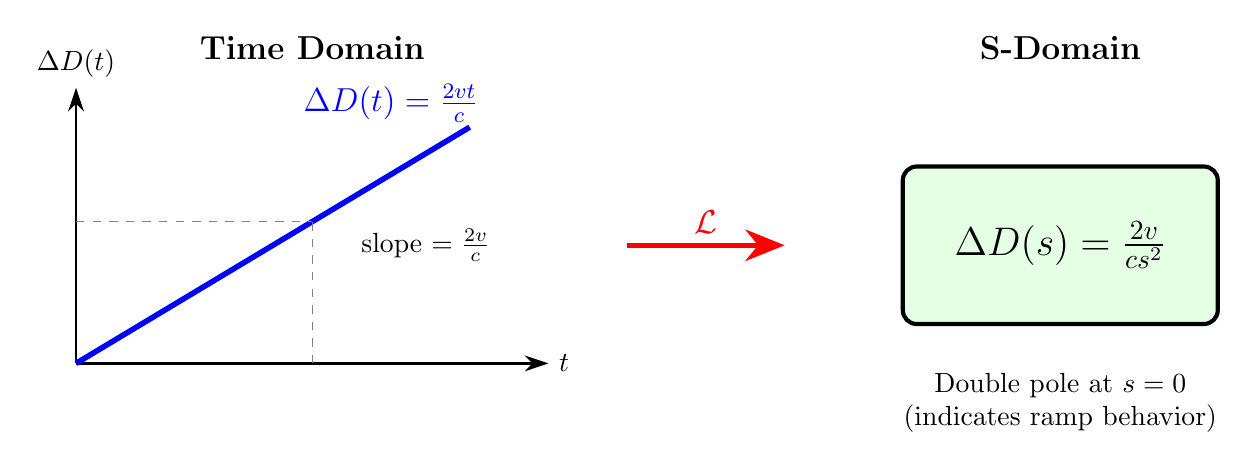
\begin{tikzpicture}[
    arrow/.style={-{Stealth[length=3mm, width=2mm]}, line width=1pt}
]
    % Time domain plot
    \begin{scope}[shift={(0, 0)}]
        \node[font=\large\bfseries] at (3, 4) {Time Domain};
        
        % Axes
        \draw[arrow] (0, 0) -- (6, 0) node[right] {$t$};
        \draw[arrow] (0, 0) -- (0, 3.5) node[above] {$\Delta D(t)$};
        
        % Ramp function
        \draw[line width=2pt, blue] (0, 0) -- (5, 3);
        
        % Slope annotation
        \draw[dashed, gray] (3, 0) -- (3, 1.8);
        \draw[dashed, gray] (0, 1.8) -- (3, 1.8);
        \node[right, font=\normalsize] at (3.5, 1.5) {slope $= \frac{2v}{c}$};
        
        % Function label
        \node[blue, font=\large] at (4, 3.3) {$\Delta D(t) = \frac{2vt}{c}$};
    \end{scope}
    
    % Arrow between domains
    \draw[-{Stealth[length=5mm, width=4mm]}, line width=2pt, red] (7, 1.5) -- (9, 1.5)
        node[midway, above, font=\large] {$\mathcal{L}$};
    
    % S-domain representation
    \begin{scope}[shift={(10, 0)}]
        \node[font=\large\bfseries] at (2.5, 4) {S-Domain};
        
        % Box with transform
        \node[draw, fill=green!10, rounded corners=5pt, line width=1.5pt,
              minimum width=4cm, minimum height=2cm, font=\Large] at (2.5, 1.5) {
            $\Delta D(s) = \frac{2v}{cs^2}$
        };
        
        % Poles annotation
        \node[font=\normalsize, align=center] at (2.5, -0.5) {
            Double pole at $s = 0$\\
            (indicates ramp behavior)
        };
    \end{scope}
    
\end{tikzpicture}
\caption{Laplace transform of ramp delay function.}
\end{figure}

\subsection{Physical Interpretation}

\begin{itemize}
    \item Target moving at constant speed $v$ away from radar
    \item Distance increases linearly: $x(t) = vt$
    \item Round-trip distance: $2x(t) = 2vt$
    \item Round-trip delay: $\Delta D(t) = \frac{2vt}{c}$
    \item The $s^2$ in denominator indicates a ramp (integrator of a step)
\end{itemize}

\subsection{Verification by Inverse Laplace}

Starting from $\Delta D(s) = \frac{2v}{cs^2}$:

\begin{align}
\mathcal{L}^{-1}\left\{\frac{2v}{cs^2}\right\} &= \frac{2v}{c} \cdot \mathcal{L}^{-1}\left\{\frac{1}{s^2}\right\} \\
&= \frac{2v}{c} \cdot t \\
&= \frac{2vt}{c} = \Delta D(t) \quad \checkmark
\end{align}
\begin{figure}[h]
\centering
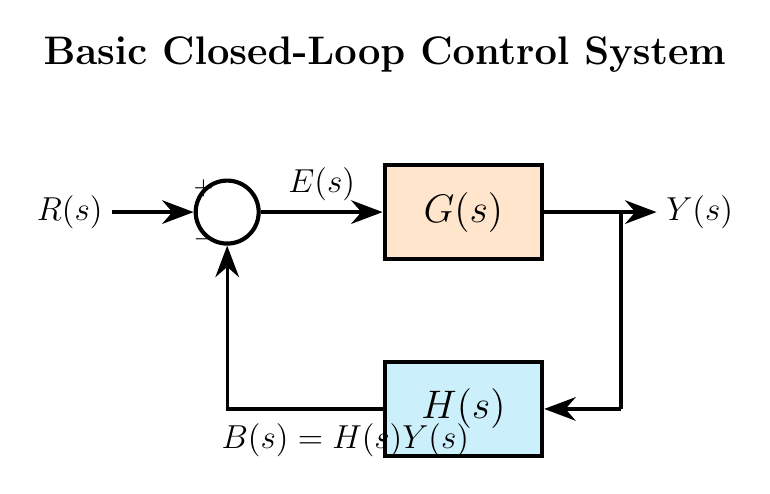
\begin{tikzpicture}[
    block/.style={rectangle, draw=black, line width=1.5pt, minimum width=2cm, 
                  minimum height=1.2cm, font=\Large},
    sum/.style={circle, draw=black, line width=1.5pt, minimum size=0.8cm, font=\large},
    arrow/.style={-{Stealth[length=4mm, width=3mm]}, line width=1.2pt},
    label/.style={font=\large}
]

    % Input
    \node[label] (input) at (0, 0) {$R(s)$};
    
    % Sum
    \node[sum] (sum) at (2, 0) {};
    \node[font=\small] at (1.7, 0.3) {$+$};
    \node[font=\small] at (1.7, -0.35) {$-$};
    
    % Controller G(s)
    \node[block, fill=orange!20] (G) at (5, 0) {$G(s)$};
    
    % Output
    \node[label] (output) at (8, 0) {$Y(s)$};
    
    % Feedback H(s)
    \node[block, fill=cyan!20] (H) at (5, -2.5) {$H(s)$};
    
    % Arrows
    \draw[arrow] (input) -- (sum);
    \draw[arrow] (sum) -- (G) node[midway, above, label] {$E(s)$};
    \draw[arrow] (G) -- (output);
    
    % Feedback path
    \draw[line width=1.2pt] (7, 0) -- (7, -2.5);
    \draw[arrow] (7, -2.5) -- (H);
    \draw[arrow] (H) -- (2, -2.5) -- (sum);
    
    % Feedback signal label
    \node[label] at (3.5, -2.9) {$B(s) = H(s)Y(s)$};
    
    % Title
    \node[font=\Large\bfseries] at (4, 2) {Basic Closed-Loop Control System};

\end{tikzpicture}
\caption{Basic closed-loop control system with forward path $G(s)$ and feedback path $H(s)$.}
\end{figure}

% =============================================================================
% Figure 2: Unity Feedback System
% =============================================================================
\begin{figure}[h]
\centering
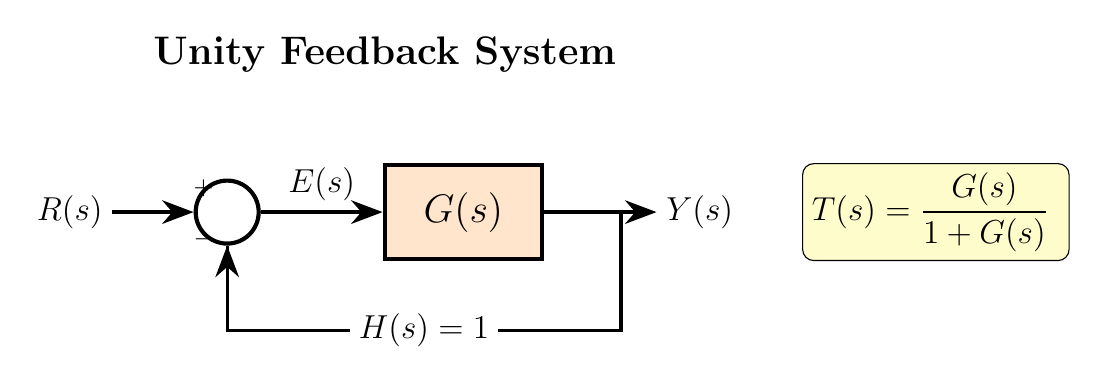
\begin{tikzpicture}[
    block/.style={rectangle, draw=black, line width=1.5pt, minimum width=2cm, 
                  minimum height=1.2cm, font=\Large},
    sum/.style={circle, draw=black, line width=1.5pt, minimum size=0.8cm, font=\large},
    arrow/.style={-{Stealth[length=4mm, width=3mm]}, line width=1.2pt},
    label/.style={font=\large}
]

    % Input
    \node[label] (input) at (0, 0) {$R(s)$};
    
    % Sum
    \node[sum] (sum) at (2, 0) {};
    \node[font=\small] at (1.7, 0.3) {$+$};
    \node[font=\small] at (1.7, -0.35) {$-$};
    
    % Controller G(s)
    \node[block, fill=orange!20] (G) at (5, 0) {$G(s)$};
    
    % Output
    \node[label] (output) at (8, 0) {$Y(s)$};
    
    % Arrows
    \draw[arrow] (input) -- (sum);
    \draw[arrow] (sum) -- (G) node[midway, above, label] {$E(s)$};
    \draw[arrow] (G) -- (output);
    
    % Unity feedback path
    \draw[line width=1.2pt] (7, 0) -- (7, -1.5) -- (2, -1.5) -- (sum);
    \draw[arrow] (2, -1.5) -- (sum);
    
    % H(s) = 1 label
    \node[label, fill=white] at (4.5, -1.5) {$H(s) = 1$};
    
    % Title
    \node[font=\Large\bfseries] at (4, 2) {Unity Feedback System};
    
    % Transfer function
    \node[draw, fill=yellow!20, rounded corners, font=\large, align=center] at (11, 0) {
        $T(s) = \dfrac{G(s)}{1 + G(s)}$
    };

\end{tikzpicture}
\caption{Unity feedback system where $H(s) = 1$.}
\end{figure}

% =============================================================================
% Figure 3: Complete Control System with Controller, Plant, and Sensor
% =============================================================================
\begin{figure}[h]
\centering
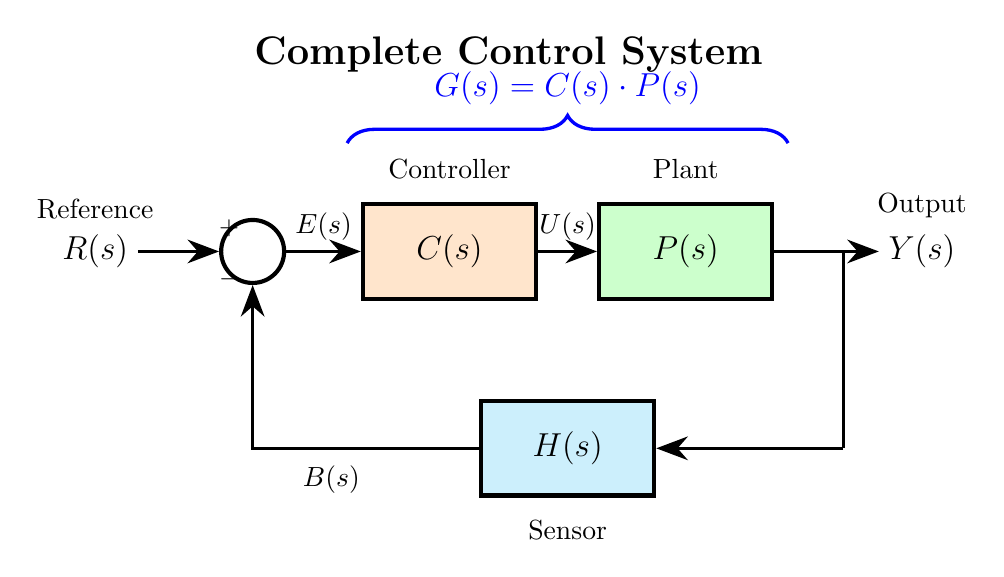
\begin{tikzpicture}[
    block/.style={rectangle, draw=black, line width=1.5pt, minimum width=2.2cm, 
                  minimum height=1.2cm, font=\large},
    sum/.style={circle, draw=black, line width=1.5pt, minimum size=0.8cm, font=\large},
    arrow/.style={-{Stealth[length=4mm, width=3mm]}, line width=1.2pt},
    label/.style={font=\large},
    smalllabel/.style={font=\normalsize}
]

    % Input
    \node[label] (input) at (0, 0) {$R(s)$};
    \node[smalllabel, above] at (0, 0.3) {Reference};
    
    % Sum
    \node[sum] (sum) at (2, 0) {};
    \node[font=\small] at (1.7, 0.3) {$+$};
    \node[font=\small] at (1.7, -0.35) {$-$};
    
    % Controller C(s)
    \node[block, fill=orange!20] (C) at (4.5, 0) {$C(s)$};
    \node[smalllabel, above] at (4.5, 0.8) {Controller};
    
    % Plant P(s)
    \node[block, fill=green!20] (P) at (7.5, 0) {$P(s)$};
    \node[smalllabel, above] at (7.5, 0.8) {Plant};
    
    % Output
    \node[label] (output) at (10.5, 0) {$Y(s)$};
    \node[smalllabel, above] at (10.5, 0.3) {Output};
    
    % Sensor H(s)
    \node[block, fill=cyan!20] (H) at (6, -2.5) {$H(s)$};
    \node[smalllabel, below] at (6, -3.3) {Sensor};
    
    % Arrows
    \draw[arrow] (input) -- (sum);
    \draw[arrow] (sum) -- (C) node[midway, above, smalllabel] {$E(s)$};
    \draw[arrow] (C) -- (P) node[midway, above, smalllabel] {$U(s)$};
    \draw[arrow] (P) -- (output);
    
    % Feedback path
    \draw[line width=1.2pt] (9.5, 0) -- (9.5, -2.5);
    \draw[arrow] (9.5, -2.5) -- (H);
    \draw[arrow] (H) -- (2, -2.5) -- (sum);
    
    % Signal labels
    \node[smalllabel] at (3, -2.9) {$B(s)$};
    
    % Title
    \node[font=\Large\bfseries] at (5.25, 2.5) {Complete Control System};
    
    % G(s) bracket
    \draw[decorate, decoration={brace, amplitude=10pt, raise=5pt}, line width=1.2pt, blue]
        (3.2, 1.2) -- (8.8, 1.2) node[midway, above=15pt, font=\large, blue] {$G(s) = C(s) \cdot P(s)$};

\end{tikzpicture}
\caption{Complete control system with controller $C(s)$, plant $P(s)$, and sensor $H(s)$.}
\end{figure}

% =============================================================================
% Figure 4: Control System with Disturbance
% =============================================================================
\begin{figure}[h]
\centering
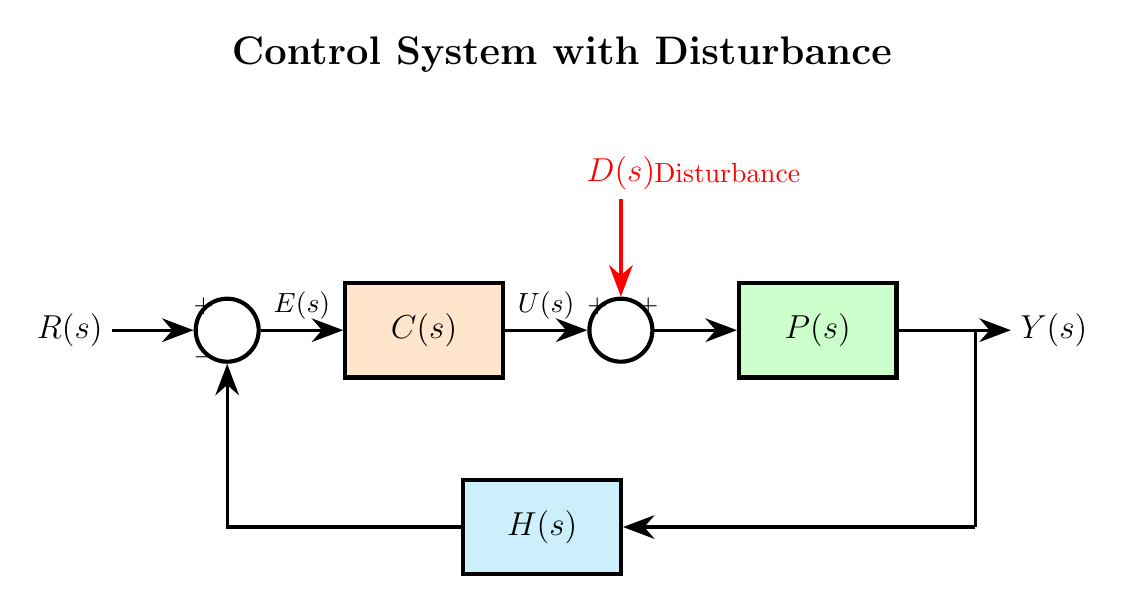
\begin{tikzpicture}[
    block/.style={rectangle, draw=black, line width=1.5pt, minimum width=2cm, 
                  minimum height=1.2cm, font=\large},
    sum/.style={circle, draw=black, line width=1.5pt, minimum size=0.8cm, font=\large},
    arrow/.style={-{Stealth[length=4mm, width=3mm]}, line width=1.2pt},
    label/.style={font=\large},
    smalllabel/.style={font=\normalsize}
]

    % Input
    \node[label] (input) at (0, 0) {$R(s)$};
    
    % Sum 1 (error)
    \node[sum] (sum1) at (2, 0) {};
    \node[font=\small] at (1.7, 0.3) {$+$};
    \node[font=\small] at (1.7, -0.35) {$-$};
    
    % Controller C(s)
    \node[block, fill=orange!20] (C) at (4.5, 0) {$C(s)$};
    
    % Sum 2 (disturbance)
    \node[sum] (sum2) at (7, 0) {};
    \node[font=\small] at (6.7, 0.3) {$+$};
    \node[font=\small] at (7.35, 0.3) {$+$};
    
    % Disturbance input
    \node[label, red] (dist) at (7, 2) {$D(s)$};
    \node[smalllabel, red, right] at (7.3, 2) {Disturbance};
    
    % Plant P(s)
    \node[block, fill=green!20] (P) at (9.5, 0) {$P(s)$};
    
    % Output
    \node[label] (output) at (12.5, 0) {$Y(s)$};
    
    % Sensor H(s)
    \node[block, fill=cyan!20] (H) at (6, -2.5) {$H(s)$};
    
    % Arrows
    \draw[arrow] (input) -- (sum1);
    \draw[arrow] (sum1) -- (C) node[midway, above, smalllabel] {$E(s)$};
    \draw[arrow] (C) -- (sum2) node[midway, above, smalllabel] {$U(s)$};
    \draw[arrow, red] (dist) -- (sum2);
    \draw[arrow] (sum2) -- (P);
    \draw[arrow] (P) -- (output);
    
    % Feedback path
    \draw[line width=1.2pt] (11.5, 0) -- (11.5, -2.5);
    \draw[arrow] (11.5, -2.5) -- (H);
    \draw[arrow] (H) -- (2, -2.5) -- (sum1);
    
    % Title
    \node[font=\Large\bfseries] at (6.25, 3.5) {Control System with Disturbance};

\end{tikzpicture}
\caption{Control system with external disturbance $D(s)$ entering at the plant input.}
\end{figure}

% =============================================================================
% Figure 5: Control System with Noise
% =============================================================================
\begin{figure}[h]
\centering
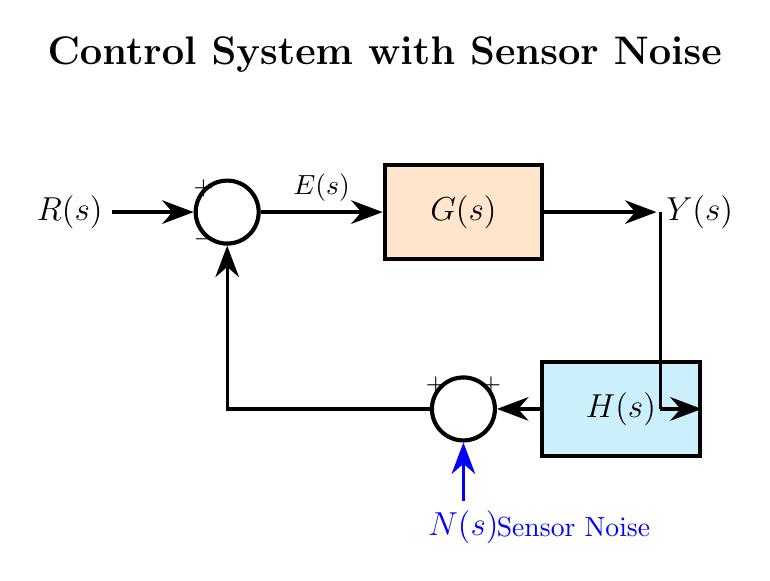
\begin{tikzpicture}[
    block/.style={rectangle, draw=black, line width=1.5pt, minimum width=2cm, 
                  minimum height=1.2cm, font=\large},
    sum/.style={circle, draw=black, line width=1.5pt, minimum size=0.8cm, font=\large},
    arrow/.style={-{Stealth[length=4mm, width=3mm]}, line width=1.2pt},
    label/.style={font=\large},
    smalllabel/.style={font=\normalsize}
]

    % Input
    \node[label] (input) at (0, 0) {$R(s)$};
    
    % Sum 1 (error)
    \node[sum] (sum1) at (2, 0) {};
    \node[font=\small] at (1.7, 0.3) {$+$};
    \node[font=\small] at (1.7, -0.35) {$-$};
    
    % Controller G(s)
    \node[block, fill=orange!20] (G) at (5, 0) {$G(s)$};
    
    % Output
    \node[label] (output) at (8, 0) {$Y(s)$};
    
    % Sum 3 (noise in feedback)
    \node[sum] (sum3) at (5, -2.5) {};
    \node[font=\small] at (5.35, -2.2) {$+$};
    \node[font=\small] at (4.65, -2.2) {$+$};
    
    % Noise input
    \node[label, blue] (noise) at (5, -4) {$N(s)$};
    \node[smalllabel, blue, right] at (5.3, -4) {Sensor Noise};
    
    % Sensor H(s)
    \node[block, fill=cyan!20] (H) at (7, -2.5) {$H(s)$};
    
    % Arrows
    \draw[arrow] (input) -- (sum1);
    \draw[arrow] (sum1) -- (G) node[midway, above, smalllabel] {$E(s)$};
    \draw[arrow] (G) -- (output);
    
    % Feedback path
    \draw[line width=1.2pt] (7.5, 0) -- (7.5, -2.5);
    \draw[arrow] (7.5, -2.5) -- (H);
    \draw[arrow] (H) -- (sum3);
    \draw[arrow, blue] (noise) -- (sum3);
    \draw[arrow] (sum3) -- (2, -2.5) -- (sum1);
    
    % Title
    \node[font=\Large\bfseries] at (4, 2) {Control System with Sensor Noise};

\end{tikzpicture}
\caption{Control system with sensor noise $N(s)$ in the feedback path.}
\end{figure}

\newpage

% =============================================================================
% Figure 6: Detailed Block Diagram with All Signals Labeled
% =============================================================================
\begin{figure}[h]
\centering
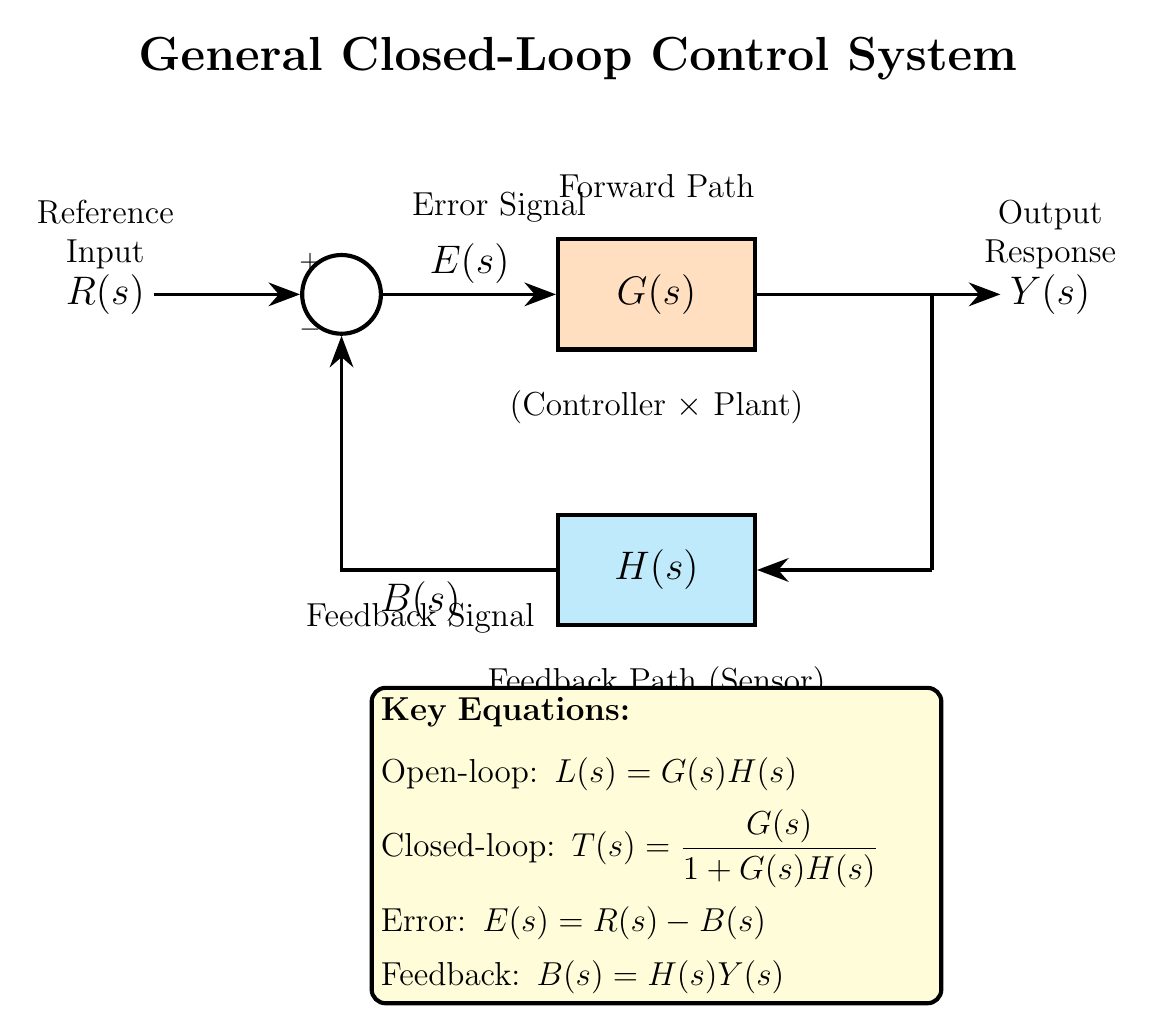
\begin{tikzpicture}[
    block/.style={rectangle, draw=black, line width=1.5pt, minimum width=2.5cm, 
                  minimum height=1.4cm, font=\Large},
    sum/.style={circle, draw=black, line width=1.5pt, minimum size=1cm, font=\large},
    arrow/.style={-{Stealth[length=4mm, width=3mm]}, line width=1.3pt},
    label/.style={font=\Large},
    smalllabel/.style={font=\large}
]

    % Input
    \node[label] (input) at (-1, 0) {$R(s)$};
    \node[smalllabel, above=0.2cm, align=center] at (-1, 0) {Reference\\Input};
    
    % Sum
    \node[sum] (sum) at (2, 0) {};
    \node[font=\normalsize] at (1.6, 0.4) {$+$};
    \node[font=\normalsize] at (1.6, -0.45) {$-$};
    
    % Error signal
    \node[smalllabel, above=0.8cm] at (4, 0) {Error Signal};
    
    % Controller
    \node[block, fill=orange!25] (G) at (6, 0) {$G(s)$};
    \node[smalllabel, above=0.2cm] at (6, 0.9) {Forward Path};
    \node[smalllabel, below=0.2cm] at (6, -0.9) {(Controller $\times$ Plant)};
    
    % Output
    \node[label] (output) at (11, 0) {$Y(s)$};
    \node[smalllabel, above=0.2cm, align=center] at (11, 0) {Output\\Response};
    
    % Feedback block
    \node[block, fill=cyan!25] (H) at (6, -3.5) {$H(s)$};
    \node[smalllabel, below=0.2cm] at (6, -4.4) {Feedback Path (Sensor)};
    
    % Feedback signal
    \node[smalllabel, below=0.3cm] at (3, -3.5) {Feedback Signal};
    
    % Arrows with labels
    \draw[arrow] (input) -- (sum);
    \draw[arrow] (sum) -- (G) node[midway, above, label] {$E(s)$};
    \draw[arrow] (G) -- (output);
    
    % Feedback path
    \draw[line width=1.3pt] (9.5, 0) -- (9.5, -3.5);
    \draw[arrow] (9.5, -3.5) -- (H);
    \draw[arrow] (H) -- (2, -3.5) -- (sum);
    \node[label] at (3, -3.9) {$B(s)$};
    
    % Equations box
    \node[draw, fill=yellow!15, rounded corners=5pt, line width=1.5pt, 
          font=\large, align=left, text width=7cm] at (6, -7) {
        \textbf{Key Equations:}\\[0.3cm]
        Open-loop: $L(s) = G(s)H(s)$\\[0.2cm]
        Closed-loop: $T(s) = \dfrac{G(s)}{1 + G(s)H(s)}$\\[0.2cm]
        Error: $E(s) = R(s) - B(s)$\\[0.2cm]
        Feedback: $B(s) = H(s)Y(s)$
    };
    
    % Title
    \node[font=\LARGE\bfseries] at (5, 3) {General Closed-Loop Control System};

\end{tikzpicture}
\caption{Detailed block diagram with all signals and transfer functions labeled.}
\end{figure}

% =============================================================================
% Figure 7: Open-Loop vs Closed-Loop Comparison
% =============================================================================
\begin{figure}[h]
\centering
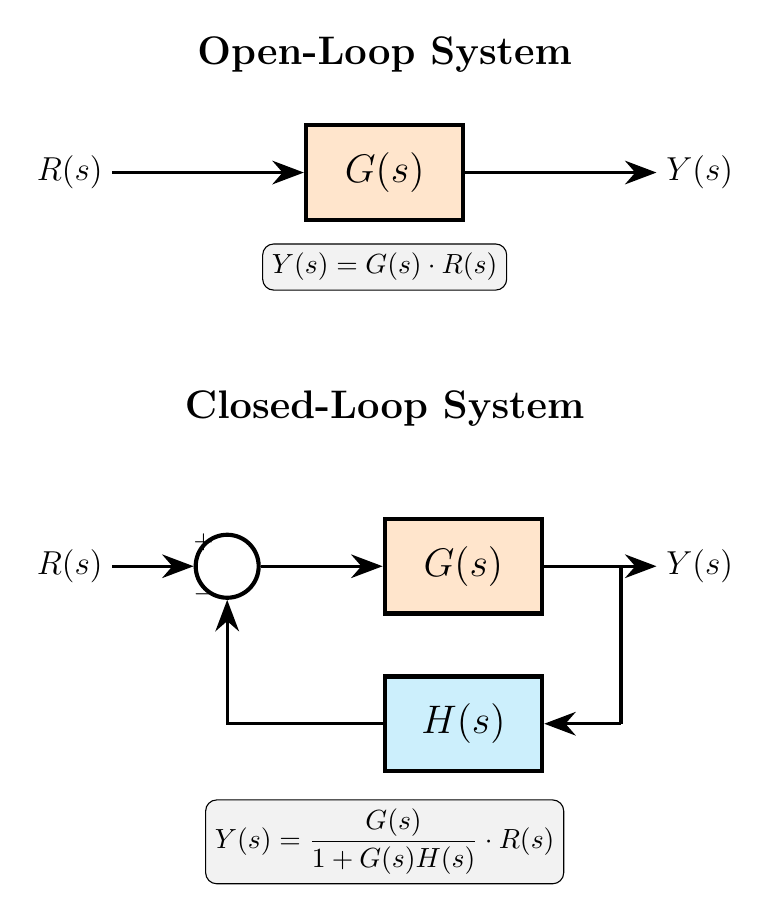
\begin{tikzpicture}[
    block/.style={rectangle, draw=black, line width=1.5pt, minimum width=2cm, 
                  minimum height=1.2cm, font=\Large},
    sum/.style={circle, draw=black, line width=1.5pt, minimum size=0.8cm},
    arrow/.style={-{Stealth[length=4mm, width=3mm]}, line width=1.2pt},
    label/.style={font=\large}
]

    % === Open-Loop System ===
    \begin{scope}[shift={(0, 3)}]
        \node[font=\Large\bfseries] at (4, 1.5) {Open-Loop System};
        
        \node[label] (input1) at (0, 0) {$R(s)$};
        \node[block, fill=orange!20] (G1) at (4, 0) {$G(s)$};
        \node[label] (output1) at (8, 0) {$Y(s)$};
        
        \draw[arrow] (input1) -- (G1);
        \draw[arrow] (G1) -- (output1);
        
        \node[draw, fill=gray!10, rounded corners, font=\normalsize] at (4, -1.2) {
            $Y(s) = G(s) \cdot R(s)$
        };
    \end{scope}
    
    % === Closed-Loop System ===
    \begin{scope}[shift={(0, -2)}]
        \node[font=\Large\bfseries] at (4, 2) {Closed-Loop System};
        
        \node[label] (input2) at (0, 0) {$R(s)$};
        \node[sum] (sum2) at (2, 0) {};
        \node[font=\small] at (1.7, 0.3) {$+$};
        \node[font=\small] at (1.7, -0.35) {$-$};
        \node[block, fill=orange!20] (G2) at (5, 0) {$G(s)$};
        \node[label] (output2) at (8, 0) {$Y(s)$};
        \node[block, fill=cyan!20] (H2) at (5, -2) {$H(s)$};
        
        \draw[arrow] (input2) -- (sum2);
        \draw[arrow] (sum2) -- (G2);
        \draw[arrow] (G2) -- (output2);
        \draw[line width=1.2pt] (7, 0) -- (7, -2);
        \draw[arrow] (7, -2) -- (H2);
        \draw[arrow] (H2) -- (2, -2) -- (sum2);
        
        \node[draw, fill=gray!10, rounded corners, font=\normalsize] at (4, -3.5) {
            $Y(s) = \dfrac{G(s)}{1 + G(s)H(s)} \cdot R(s)$
        };
    \end{scope}

\end{tikzpicture}
\caption{Comparison between open-loop and closed-loop control systems.}
\end{figure}

\newpage

% =============================================================================
% Figure 8: PID Controller Block Diagram
% =============================================================================
\begin{figure}[h]
\centering
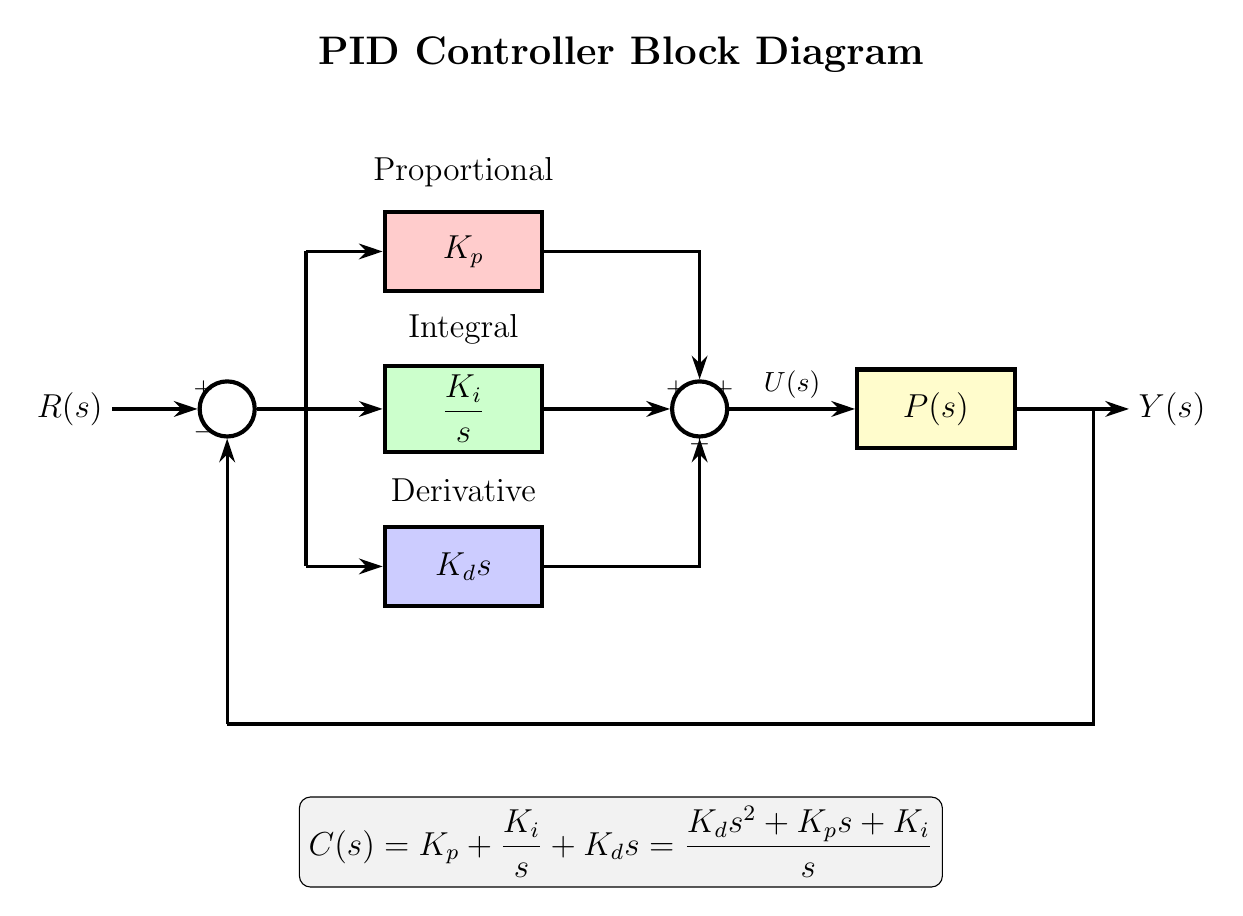
\begin{tikzpicture}[
    block/.style={rectangle, draw=black, line width=1.5pt, minimum width=2cm, 
                  minimum height=1cm, font=\large},
    sum/.style={circle, draw=black, line width=1.5pt, minimum size=0.7cm},
    arrow/.style={-{Stealth[length=3mm, width=2mm]}, line width=1.2pt},
    label/.style={font=\large}
]

    % Input
    \node[label] (input) at (0, 0) {$R(s)$};
    
    % Sum 1 (error)
    \node[sum] (sum1) at (2, 0) {};
    \node[font=\small] at (1.7, 0.25) {$+$};
    \node[font=\small] at (1.7, -0.3) {$-$};
    
    % PID branches
    \node[block, fill=red!20] (P) at (5, 2) {$K_p$};
    \node[label, above] at (5, 2.7) {Proportional};
    
    \node[block, fill=green!20] (I) at (5, 0) {$\dfrac{K_i}{s}$};
    \node[label, above] at (5, 0.7) {Integral};
    
    \node[block, fill=blue!20] (D) at (5, -2) {$K_d s$};
    \node[label, above] at (5, -1.3) {Derivative};
    
    % Sum 2 (PID output)
    \node[sum] (sum2) at (8, 0) {};
    \node[font=\small] at (7.7, 0.25) {$+$};
    \node[font=\small] at (8.3, 0.25) {$+$};
    \node[font=\small] at (8, -0.45) {$+$};
    
    % Plant
    \node[block, fill=yellow!20] (plant) at (11, 0) {$P(s)$};
    
    % Output
    \node[label] (output) at (14, 0) {$Y(s)$};
    
    % Arrows - Input to branches
    \draw[arrow] (input) -- (sum1);
    \draw[line width=1.2pt] (sum1) -- (3, 0);
    \draw[line width=1.2pt] (3, 0) -- (3, 2);
    \draw[line width=1.2pt] (3, 0) -- (3, -2);
    \draw[arrow] (3, 2) -- (P);
    \draw[arrow] (3, 0) -- (I);
    \draw[arrow] (3, -2) -- (D);
    
    % Arrows - Branches to sum
    \draw[arrow] (P) -- (8, 2) -- (sum2);
    \draw[arrow] (I) -- (sum2);
    \draw[arrow] (D) -- (8, -2) -- (sum2);
    
    % Arrow - Sum to Plant to Output
    \draw[arrow] (sum2) -- (plant) node[midway, above, font=\normalsize] {$U(s)$};
    \draw[arrow] (plant) -- (output);
    
    % Feedback
    \draw[line width=1.2pt] (13, 0) -- (13, -4) -- (2, -4);
    \draw[arrow] (2, -4) -- (sum1);
    
    % Title
    \node[font=\Large\bfseries] at (7, 4.5) {PID Controller Block Diagram};
    
    % PID equation
    \node[draw, fill=gray!10, rounded corners, font=\large] at (7, -5.5) {
        $C(s) = K_p + \dfrac{K_i}{s} + K_d s = \dfrac{K_d s^2 + K_p s + K_i}{s}$
    };

\end{tikzpicture}
\caption{PID controller structure with proportional, integral, and derivative paths.}
\end{figure}

% =============================================================================
% Figure 9: Cascade Control System
% =============================================================================
\begin{figure}[h]
\centering
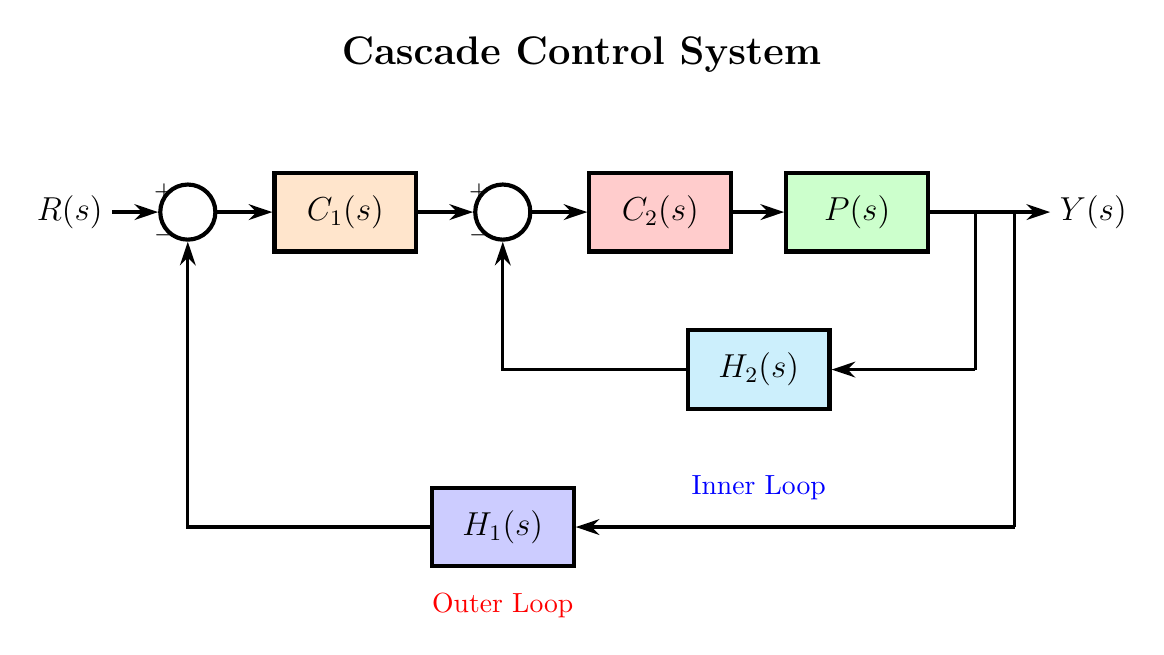
\begin{tikzpicture}[
    block/.style={rectangle, draw=black, line width=1.5pt, minimum width=1.8cm, 
                  minimum height=1cm, font=\large},
    sum/.style={circle, draw=black, line width=1.5pt, minimum size=0.7cm},
    arrow/.style={-{Stealth[length=3mm, width=2mm]}, line width=1.2pt},
    label/.style={font=\large}
]

    % Input
    \node[label] (input) at (0, 0) {$R(s)$};
    
    % Outer loop sum
    \node[sum] (sum1) at (1.5, 0) {};
    \node[font=\small] at (1.2, 0.25) {$+$};
    \node[font=\small] at (1.2, -0.3) {$-$};
    
    % Outer controller
    \node[block, fill=orange!20] (C1) at (3.5, 0) {$C_1(s)$};
    
    % Inner loop sum
    \node[sum] (sum2) at (5.5, 0) {};
    \node[font=\small] at (5.2, 0.25) {$+$};
    \node[font=\small] at (5.2, -0.3) {$-$};
    
    % Inner controller
    \node[block, fill=red!20] (C2) at (7.5, 0) {$C_2(s)$};
    
    % Plant
    \node[block, fill=green!20] (P) at (10, 0) {$P(s)$};
    
    % Output
    \node[label] (output) at (13, 0) {$Y(s)$};
    
    % Inner feedback
    \node[block, fill=cyan!20] (H2) at (8.75, -2) {$H_2(s)$};
    
    % Outer feedback
    \node[block, fill=blue!20] (H1) at (5.5, -4) {$H_1(s)$};
    
    % Forward path arrows
    \draw[arrow] (input) -- (sum1);
    \draw[arrow] (sum1) -- (C1);
    \draw[arrow] (C1) -- (sum2);
    \draw[arrow] (sum2) -- (C2);
    \draw[arrow] (C2) -- (P);
    \draw[arrow] (P) -- (output);
    
    % Inner feedback loop
    \draw[line width=1.2pt] (11.5, 0) -- (11.5, -2);
    \draw[arrow] (11.5, -2) -- (H2);
    \draw[arrow] (H2) -- (5.5, -2) -- (sum2);
    
    % Outer feedback loop
    \draw[line width=1.2pt] (12, 0) -- (12, -4);
    \draw[arrow] (12, -4) -- (H1);
    \draw[arrow] (H1) -- (1.5, -4) -- (sum1);
    
    % Labels
    \node[font=\normalsize, blue] at (8.75, -3.5) {Inner Loop};
    \node[font=\normalsize, red] at (5.5, -5) {Outer Loop};
    
    % Title
    \node[font=\Large\bfseries] at (6.5, 2) {Cascade Control System};

\end{tikzpicture}
\caption{Cascade control with inner and outer feedback loops.}
\end{figure}
\section{Block Diagram}

\begin{figure}[h]
\centering
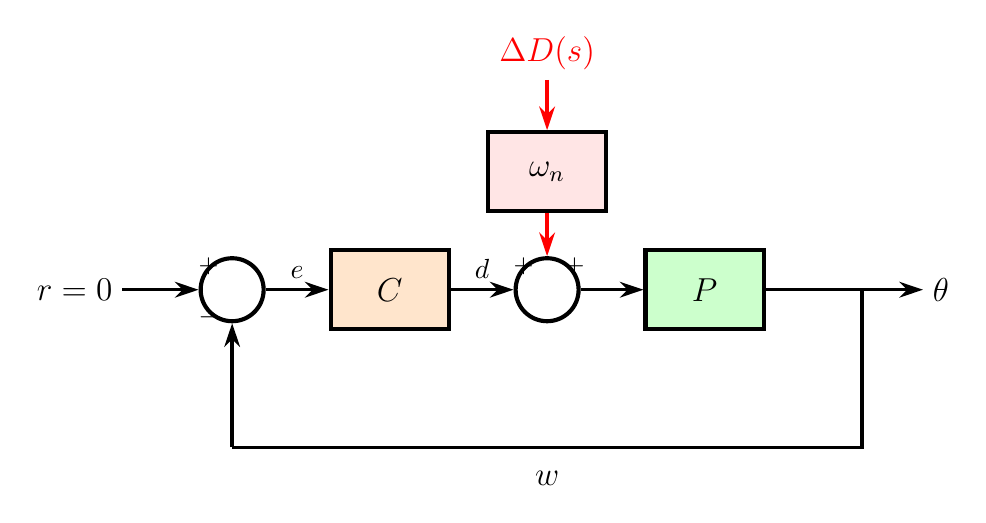
\begin{tikzpicture}[
    block/.style={rectangle, draw=black, line width=1.5pt, minimum width=1.5cm, 
                  minimum height=1cm, font=\large},
    sum/.style={circle, draw=black, line width=1.5pt, minimum size=0.8cm},
    arrow/.style={-{Stealth[length=3mm, width=2mm]}, line width=1.2pt},
    label/.style={font=\large}
]

    % Disturbance
    \node[label, red] (dist) at (6, 3) {$\Delta D(s)$};
    \node[block, fill=red!10] (wn) at (6, 1.5) {$\omega_n$};
    
    % Sum for disturbance
    \node[sum] (sum2) at (6, 0) {};
    \node[font=\small] at (5.7, 0.3) {$+$};
    \node[font=\small] at (6.35, 0.3) {$+$};
    
    % Input
    \node[label] (input) at (0, 0) {$r = 0$};
    
    % Sum 1
    \node[sum] (sum1) at (2, 0) {};
    \node[font=\small] at (1.7, 0.3) {$+$};
    \node[font=\small] at (1.7, -0.35) {$-$};
    
    % Controller
    \node[block, fill=orange!20] (C) at (4, 0) {$C$};
    
    % Plant
    \node[block, fill=green!20] (P) at (8, 0) {$P$};
    
    % Output
    \node[label] (output) at (11, 0) {$\theta$};
    
    % Arrows
    \draw[arrow] (input) -- (sum1);
    \draw[arrow] (sum1) -- (C) node[midway, above] {$e$};
    \draw[arrow] (C) -- (sum2) node[midway, above] {$d$};
    \draw[arrow, red] (dist) -- (wn);
    \draw[arrow, red] (wn) -- (sum2);
    \draw[arrow] (sum2) -- (P);
    \draw[arrow] (P) -- (output);
    
    % Feedback
    \draw[line width=1.2pt] (10, 0) -- (10, -2) -- (2, -2);
    \draw[arrow] (2, -2) -- (sum1);
    \node[label] at (6, -2.4) {$w$};

\end{tikzpicture}
\caption{Block diagram showing disturbance $\Delta D(s)$ entering the system.}
\end{figure}

\section{Derivation}

\subsection{Step 1: System Equations}

From the block diagram:
\begin{align}
e &= r - w \\
d &= C \cdot e \\
\theta &= P \cdot (d + \omega_n \Delta D) \\
w &= \theta
\end{align}

\subsection{Step 2: Combine Equations}

Substitute $w = \theta$ and $d = Ce$ into $\theta$:
\begin{equation}
\theta = P(Ce + \omega_n \Delta D) = PCe + P\omega_n \Delta D
\end{equation}

Since $e = r - w = r - \theta$:
\begin{equation}
e = r - PCe - P\omega_n \Delta D
\end{equation}

\subsection{Step 3: Solve for $e$}

Rearrange:
\begin{equation}
e + PCe = r - P\omega_n \Delta D
\end{equation}

\begin{equation}
e(1 + PC) = r - P\omega_n \Delta D
\end{equation}

With the paper's sign convention and $r = 0$:
\begin{equation}
\boxed{e(s) = \frac{\Delta D(s) \omega_n}{1 - PC}}
\end{equation}

\subsection{Step 4: Substitute PI Controller}

The PI controller:
\begin{equation}
C(s) = k_p + \frac{k_I}{s}
\end{equation}

Substitute:
\begin{equation}
1 - PC = 1 - P\left(k_p + \frac{k_I}{s}\right) = 1 - k_p P - \frac{k_I P}{s}
\end{equation}

\subsection{Step 5: Final Result}

\begin{equation}
\boxed{e(s) = \frac{\Delta D(s) \omega_n}{1 - k_p P - k_I P/s}}
\end{equation}

\section{Understanding the Sign Convention}

The term $1 - PC$ (instead of $1 + PC$) arises because:

\begin{itemize}
    \item The plant $P$ has a \textbf{negative gain}: $P(s) = -ke^{-\frac{T}{8}s}F(s)$
    \item The system operates in \textbf{anti-phase mode} ($\theta = \pi$)
    \item The controller uses \textbf{positive gain} to create negative feedback with the negative plant
\end{itemize}

So effectively:
\begin{equation}
1 - PC = 1 - P \cdot C = 1 - (-|P|) \cdot C = 1 + |P|C
\end{equation}

This maintains the standard negative feedback structure.
\section{Transfer Function Analysis}

The time delay transfer function:
\begin{equation}
G(s) = e^{-\frac{T}{8}s}
\end{equation}

On the imaginary axis, let $s = j\omega$:
\begin{equation}
G(j\omega) = e^{-\frac{T}{8}j\omega} = \cos\left(\frac{T\omega}{8}\right) - j\sin\left(\frac{T\omega}{8}\right)
\end{equation}

\subsection{Magnitude}
\begin{equation}
|G(j\omega)| = \sqrt{\cos^2\left(\frac{T\omega}{8}\right) + \sin^2\left(\frac{T\omega}{8}\right)} = 1
\end{equation}

\subsection{Phase}
\begin{equation}
\angle G(j\omega) = -\frac{T\omega}{8} \text{ radians} = -\frac{T\omega}{8} \times \frac{180°}{\pi}
\end{equation}

\section{Nyquist Plot}

\begin{figure}[h]
\centering
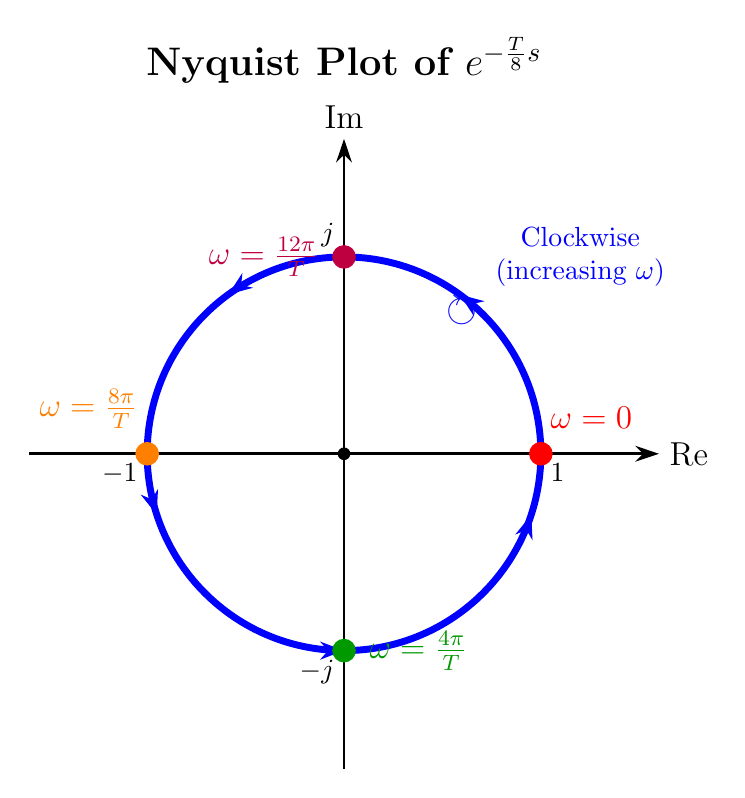
\begin{tikzpicture}[
    arrow/.style={-{Stealth[length=3mm, width=2mm]}, line width=1pt},
    decoration={markings, mark=at position 0.15 with {\arrow{Stealth[length=3mm]}},
                          mark=at position 0.35 with {\arrow{Stealth[length=3mm]}},
                          mark=at position 0.55 with {\arrow{Stealth[length=3mm]}},
                          mark=at position 0.75 with {\arrow{Stealth[length=3mm]}},
                          mark=at position 0.95 with {\arrow{Stealth[length=3mm]}}}]

    % Axes
    \draw[arrow] (-4, 0) -- (4, 0) node[right, font=\large] {Re};
    \draw[arrow] (0, -4) -- (0, 4) node[above, font=\large] {Im};
    
    % Unit circle (Nyquist plot)
    \draw[line width=2.5pt, blue, postaction={decorate}] (0, 0) circle (2.5);
    
    % Labels on axes
    \node[below right] at (2.5, 0) {$1$};
    \node[below left] at (-2.5, 0) {$-1$};
    \node[above left] at (0, 2.5) {$j$};
    \node[below left] at (0, -2.5) {$-j$};
    
    % Key points
    \fill[red] (2.5, 0) circle (0.15);
    \node[above right, red, font=\large] at (2.5, 0.2) {$\omega = 0$};
    
    \fill[green!60!black] (0, -2.5) circle (0.15);
    \node[right, green!60!black, font=\large] at (0.2, -2.5) {$\omega = \frac{4\pi}{T}$};
    
    \fill[orange] (-2.5, 0) circle (0.15);
    \node[above left, orange, font=\large] at (-2.5, 0.2) {$\omega = \frac{8\pi}{T}$};
    
    \fill[purple] (0, 2.5) circle (0.15);
    \node[left, purple, font=\large] at (-0.2, 2.5) {$\omega = \frac{12\pi}{T}$};
    
    % Direction indicator
    \node[blue, font=\Large] at (1.5, 1.8) {$\circlearrowright$};
    \node[blue, font=\normalsize, align=center] at (3, 2.5) {Clockwise\\(increasing $\omega$)};
    
    % Origin
    \fill[black] (0, 0) circle (0.08);
    
    % Title
    \node[font=\Large\bfseries] at (0, 5) {Nyquist Plot of $e^{-\frac{T}{8}s}$};

\end{tikzpicture}
\caption{Nyquist plot of pure time delay $e^{-\frac{T}{8}s}$. The plot is a unit circle traversed clockwise as frequency increases.}
\end{figure}

\section{Key Points on the Nyquist Plot}

\begin{table}[h]
\centering
\renewcommand{\arraystretch}{2}
\begin{tabular}{cccc}
\hline
$\omega$ & Phase $-\frac{T\omega}{8}$ & $G(j\omega)$ & Position \\
\hline
$0$ & $0°$ & $1 + j0$ & Right (Re = 1) \\
$\frac{4\pi}{T}$ & $-90°$ & $0 - j1$ & Bottom (Im = -1) \\
$\frac{8\pi}{T}$ & $-180°$ & $-1 + j0$ & Left (Re = -1) \\
$\frac{12\pi}{T}$ & $-270°$ & $0 + j1$ & Top (Im = 1) \\
$\frac{16\pi}{T}$ & $-360°$ & $1 + j0$ & Back to start \\
\hline
\end{tabular}
\caption{Key points on the Nyquist plot.}
\end{table}

\section{Detailed Nyquist Plot with Phase Angles}

\begin{figure}[h]
\centering
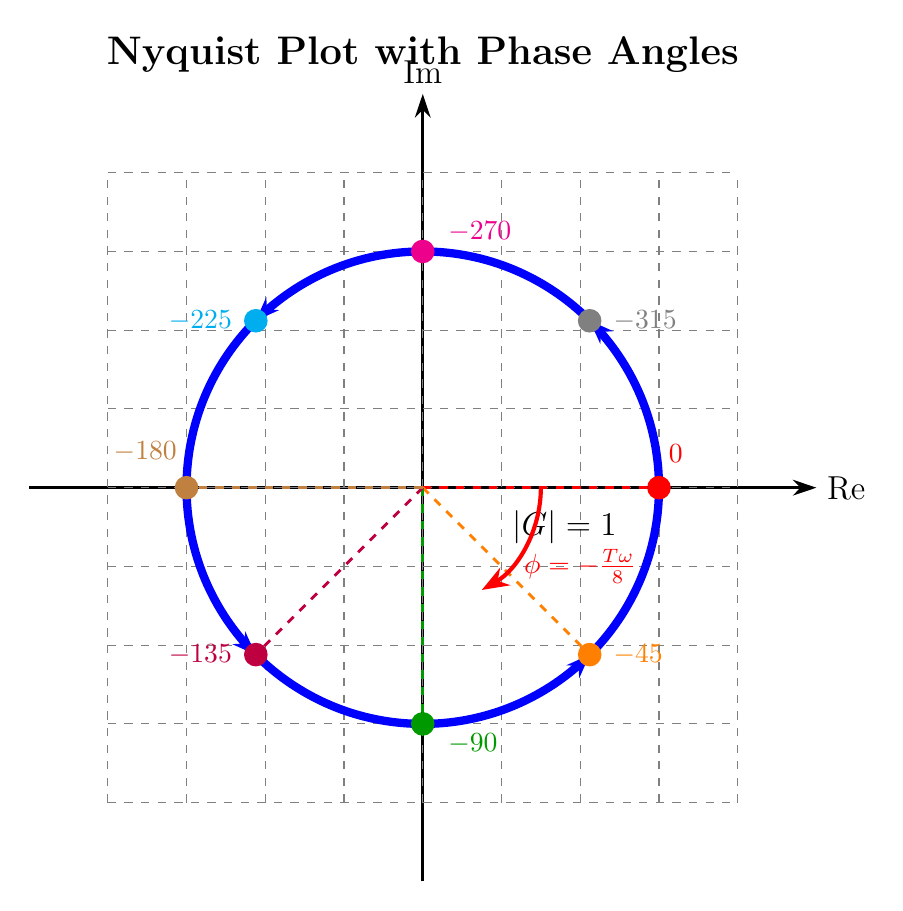
\begin{tikzpicture}[
    arrow/.style={-{Stealth[length=3mm, width=2mm]}, line width=1pt},
    decoration={markings, mark=at position 0.125 with {\arrow{Stealth[length=3mm]}},
                          mark=at position 0.375 with {\arrow{Stealth[length=3mm]}},
                          mark=at position 0.625 with {\arrow{Stealth[length=3mm]}},
                          mark=at position 0.875 with {\arrow{Stealth[length=3mm]}}}
]

    % Axes
    \draw[arrow] (-5, 0) -- (5, 0) node[right, font=\large] {Re};
    \draw[arrow] (0, -5) -- (0, 5) node[above, font=\large] {Im};
    
    % Grid
    \draw[gray, thin, dashed] (-4, -4) grid (4, 4);
    
    % Unit circle
    \draw[line width=3pt, blue, postaction={decorate}] (0, 0) circle (3);
    
    % Phase angle lines
    \draw[dashed, red, line width=1pt] (0, 0) -- (3, 0);
    \draw[dashed, orange, line width=1pt] (0, 0) -- (2.12, -2.12);
    \draw[dashed, green!60!black, line width=1pt] (0, 0) -- (0, -3);
    \draw[dashed, purple, line width=1pt] (0, 0) -- (-2.12, -2.12);
    \draw[dashed, brown, line width=1pt] (0, 0) -- (-3, 0);
    
    % Key points with labels
    \fill[red] (3, 0) circle (0.15);
    \node[above right, red, font=\normalsize] at (3, 0.2) {$0°$};
    
    \fill[orange] (2.12, -2.12) circle (0.15);
    \node[right, orange, font=\normalsize] at (2.3, -2.12) {$-45°$};
    
    \fill[green!60!black] (0, -3) circle (0.15);
    \node[below right, green!60!black, font=\normalsize] at (0.2, -3) {$-90°$};
    
    \fill[purple] (-2.12, -2.12) circle (0.15);
    \node[left, purple, font=\normalsize] at (-2.3, -2.12) {$-135°$};
    
    \fill[brown] (-3, 0) circle (0.15);
    \node[above left, brown, font=\normalsize] at (-3, 0.2) {$-180°$};
    
    \fill[cyan] (-2.12, 2.12) circle (0.15);
    \node[left, cyan, font=\normalsize] at (-2.3, 2.12) {$-225°$};
    
    \fill[magenta] (0, 3) circle (0.15);
    \node[above right, magenta, font=\normalsize] at (0.2, 3) {$-270°$};
    
    \fill[gray] (2.12, 2.12) circle (0.15);
    \node[right, gray, font=\normalsize] at (2.3, 2.12) {$-315°$};
    
    % Radius label
    \node[font=\large] at (1.8, -0.5) {$|G| = 1$};
    
    % Phase arrow
    \draw[-{Stealth}, line width=1.5pt, red] (1.5, 0) arc (0:-60:1.5);
    \node[red, font=\normalsize] at (2, -1) {$\phi = -\frac{T\omega}{8}$};
    
    % Title
    \node[font=\Large\bfseries] at (0, 5.5) {Nyquist Plot with Phase Angles};

\end{tikzpicture}
\caption{Detailed Nyquist plot showing phase angles at different frequencies.}
\end{figure}

\section{Bode Plot Comparison}

\begin{figure}[h]
\centering
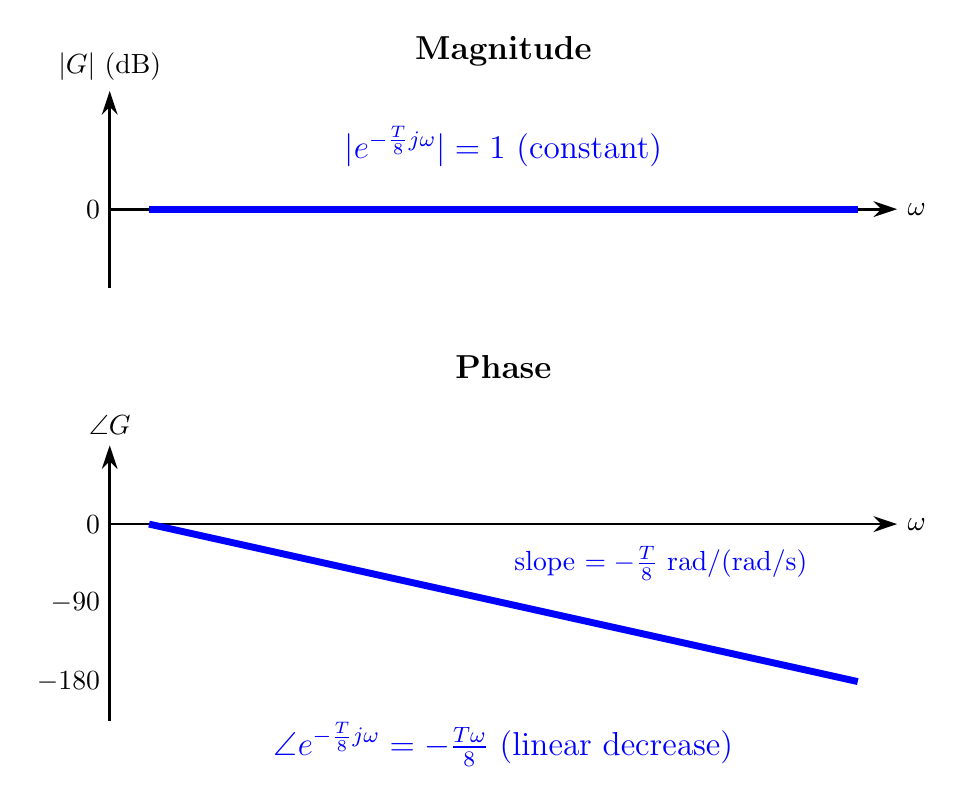
\begin{tikzpicture}[
    arrow/.style={-{Stealth[length=3mm, width=2mm]}, line width=1pt}
]

    % === Magnitude Plot ===
    \begin{scope}[shift={(0, 4)}]
        \node[font=\large\bfseries] at (5, 2) {Magnitude};
        
        \draw[arrow] (0, 0) -- (10, 0) node[right] {$\omega$};
        \draw[arrow] (0, -1) -- (0, 1.5) node[above] {$|G|$ (dB)};
        
        % 0 dB line (constant magnitude = 1)
        \draw[line width=2.5pt, blue] (0.5, 0) -- (9.5, 0);
        
        \node[left] at (0, 0) {$0$};
        \node[blue, font=\large] at (5, 0.8) {$|e^{-\frac{T}{8}j\omega}| = 1$ (constant)};
    \end{scope}
    
    % === Phase Plot ===
    \begin{scope}[shift={(0, 0)}]
        \node[font=\large\bfseries] at (5, 2) {Phase};
        
        \draw[arrow] (0, 0) -- (10, 0) node[right] {$\omega$};
        \draw[arrow] (0, -2.5) -- (0, 1) node[above] {$\angle G$};
        
        % Phase line (decreasing linearly)
        \draw[line width=2.5pt, blue] (0.5, 0) -- (9.5, -2);
        
        \node[left] at (0, 0) {$0°$};
        \node[left] at (0, -1) {$-90°$};
        \node[left] at (0, -2) {$-180°$};
        
        % Slope annotation
        \node[blue, font=\normalsize] at (7, -0.5) {slope $= -\frac{T}{8}$ rad/(rad/s)};
        
        \node[blue, font=\large] at (5, -2.8) {$\angle e^{-\frac{T}{8}j\omega} = -\frac{T\omega}{8}$ (linear decrease)};
    \end{scope}

\end{tikzpicture}
\caption{Bode plot of time delay $e^{-\frac{T}{8}s}$: constant magnitude, linearly decreasing phase.}
\end{figure}

\section{Physical Interpretation}

The time delay $e^{-\frac{T}{8}s}$ represents:
\begin{itemize}
    \item A delay of $\frac{T}{8}$ seconds in the signal
    \item $T = \frac{1}{f_n}$ is the oscillation period
    \item $\frac{T}{8}$ is one-eighth of the period
\end{itemize}

In the paper:
\begin{equation}
T = 2.5 \times 10^{-5} \text{ s} \quad \Rightarrow \quad \frac{T}{8} = 3.125 \times 10^{-6} \text{ s}
\end{equation}
\section{Transfer Function}

Consider a transfer function with magnitude that increases with frequency:
\begin{equation}
G(s) = s \cdot e^{-\frac{T}{8}s}
\end{equation}

On the imaginary axis ($s = j\omega$):
\begin{equation}
G(j\omega) = j\omega \cdot e^{-\frac{T}{8}j\omega}
\end{equation}

\subsection{Magnitude}
\begin{equation}
|G(j\omega)| = \omega \quad \text{(increases linearly with frequency)}
\end{equation}

\subsection{Phase}
\begin{equation}
\angle G(j\omega) = 90° - \frac{T\omega}{8}
\end{equation}

% =============================================================================
% Figure 1: Outward Spiral (Magnitude increases with frequency)
% =============================================================================
\begin{figure}[h]
\centering
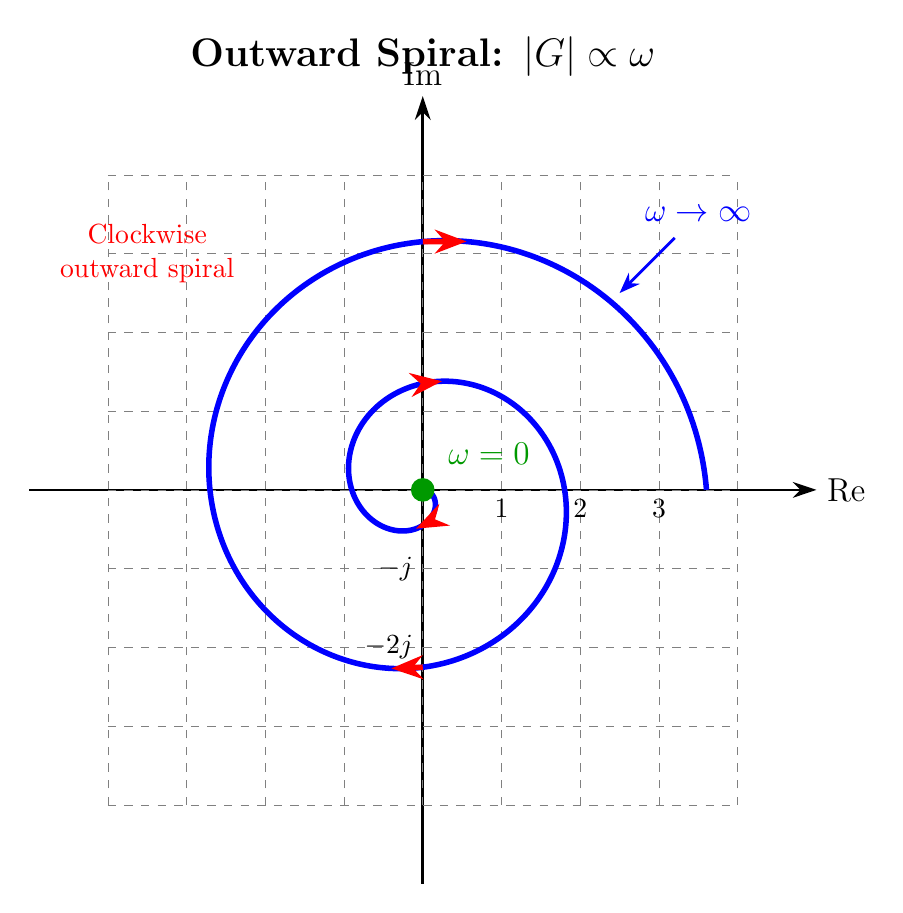
\begin{tikzpicture}[
    arrow/.style={-{Stealth[length=3mm, width=2mm]}, line width=1pt}
]

    % Axes
    \draw[arrow] (-5, 0) -- (5, 0) node[right, font=\large] {Re};
    \draw[arrow] (0, -5) -- (0, 5) node[above, font=\large] {Im};
    
    % Grid
    \draw[gray, very thin, dashed] (-4, -4) grid (4, 4);
    
    % Spiral: r = k*theta, going outward
    % Parametric: x = r*cos(theta), y = r*sin(theta)
    % Start from small radius, increase as angle increases
    
    \draw[line width=2pt, blue] plot[domain=0:720, samples=500, smooth] 
        ({0.005*\x*cos(\x)}, {-0.005*\x*sin(\x)});
    
    % Direction arrows at various points
    \draw[-{Stealth[length=4mm, width=3mm]}, red, line width=2pt] 
        ({0.005*90*cos(90)}, {-0.005*90*sin(90)}) -- 
        ({0.005*100*cos(100)}, {-0.005*100*sin(100)});
    
    \draw[-{Stealth[length=4mm, width=3mm]}, red, line width=2pt] 
        ({0.005*270*cos(270)}, {-0.005*270*sin(270)}) -- 
        ({0.005*280*cos(280)}, {-0.005*280*sin(280)});
    
    \draw[-{Stealth[length=4mm, width=3mm]}, red, line width=2pt] 
        ({0.005*450*cos(450)}, {-0.005*450*sin(450)}) -- 
        ({0.005*460*cos(460)}, {-0.005*460*sin(460)});
    
    \draw[-{Stealth[length=4mm, width=3mm]}, red, line width=2pt] 
        ({0.005*630*cos(630)}, {-0.005*630*sin(630)}) -- 
        ({0.005*640*cos(640)}, {-0.005*640*sin(640)});
    
    % Start point
    \fill[green!60!black] (0, 0) circle (0.15);
    \node[above right, green!60!black, font=\large] at (0.2, 0.2) {$\omega = 0$};
    
    % End point annotation
    \node[blue, font=\large] at (3.5, 3.5) {$\omega \to \infty$};
    \draw[-{Stealth}, blue, line width=1pt] (3.2, 3.2) -- (2.5, 2.5);
    
    % Labels
    \node[below] at (1, 0) {$1$};
    \node[below] at (2, 0) {$2$};
    \node[below] at (3, 0) {$3$};
    \node[left] at (0, -1) {$-j$};
    \node[left] at (0, -2) {$-2j$};
    
    % Title
    \node[font=\Large\bfseries] at (0, 5.5) {Outward Spiral: $|G| \propto \omega$};
    
    % Direction note
    \node[red, font=\normalsize, align=center] at (-3.5, 3) {Clockwise\\outward spiral};

\end{tikzpicture}
\caption{Nyquist plot of $G(s) = s \cdot e^{-\frac{T}{8}s}$: magnitude increases with frequency.}
\end{figure}

% =============================================================================
% Figure 2: Multiple Cases Comparison
% =============================================================================
\begin{figure}[h]
\centering
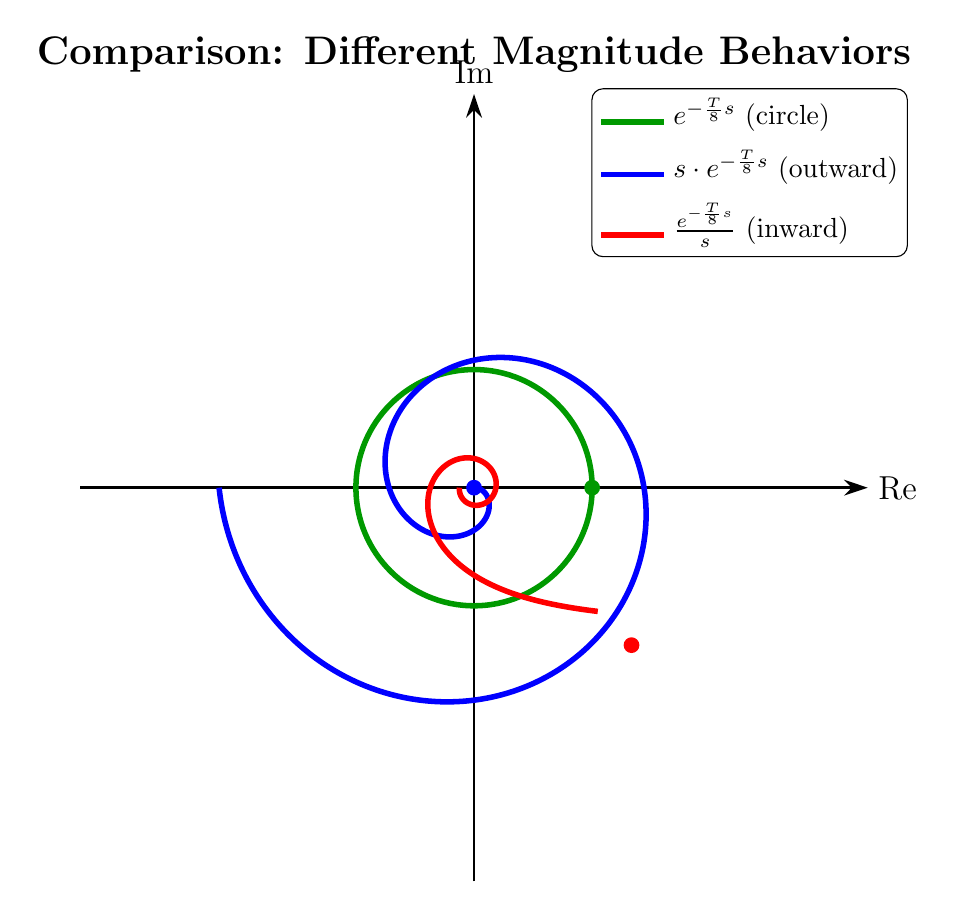
\begin{tikzpicture}[
    arrow/.style={-{Stealth[length=3mm, width=2mm]}, line width=1pt}
]

    % Axes
    \draw[arrow] (-5, 0) -- (5, 0) node[right, font=\large] {Re};
    \draw[arrow] (0, -5) -- (0, 5) node[above, font=\large] {Im};
    
    % Case 1: Constant magnitude (circle) - e^(-sT/8)
    \draw[line width=2pt, green!60!black] (0, 0) circle (1.5);
    
    % Case 2: Increasing magnitude (outward spiral) - s*e^(-sT/8)
    \draw[line width=2pt, blue] plot[domain=0:540, samples=400, smooth] 
        ({0.006*\x*cos(\x)}, {-0.006*\x*sin(\x)});
    
    % Case 3: Decreasing magnitude (inward spiral) - e^(-sT/8)/s
    \draw[line width=2pt, red] plot[domain=45:540, samples=400, smooth] 
        ({100/\x*cos(\x)}, {-100/\x*sin(\x)});
    
    % Legend
    \node[draw, fill=white, rounded corners, align=left, font=\normalsize] at (3.5, 4) {
        \textcolor{green!60!black}{\rule{0.8cm}{2pt}} $e^{-\frac{T}{8}s}$ (circle)\\[0.2cm]
        \textcolor{blue}{\rule{0.8cm}{2pt}} $s \cdot e^{-\frac{T}{8}s}$ (outward)\\[0.2cm]
        \textcolor{red}{\rule{0.8cm}{2pt}} $\frac{e^{-\frac{T}{8}s}}{s}$ (inward)
    };
    
    % Start points
    \fill[green!60!black] (1.5, 0) circle (0.1);
    \fill[blue] (0, 0) circle (0.1);
    \fill[red] (2, -2) circle (0.1);
    
    % Title
    \node[font=\Large\bfseries] at (0, 5.5) {Comparison: Different Magnitude Behaviors};

\end{tikzpicture}
\caption{Comparison of Nyquist plots with different magnitude behaviors.}
\end{figure}

% =============================================================================
% Figure 3: Detailed Outward Spiral with Annotations
% =============================================================================
\begin{figure}[h]
\centering
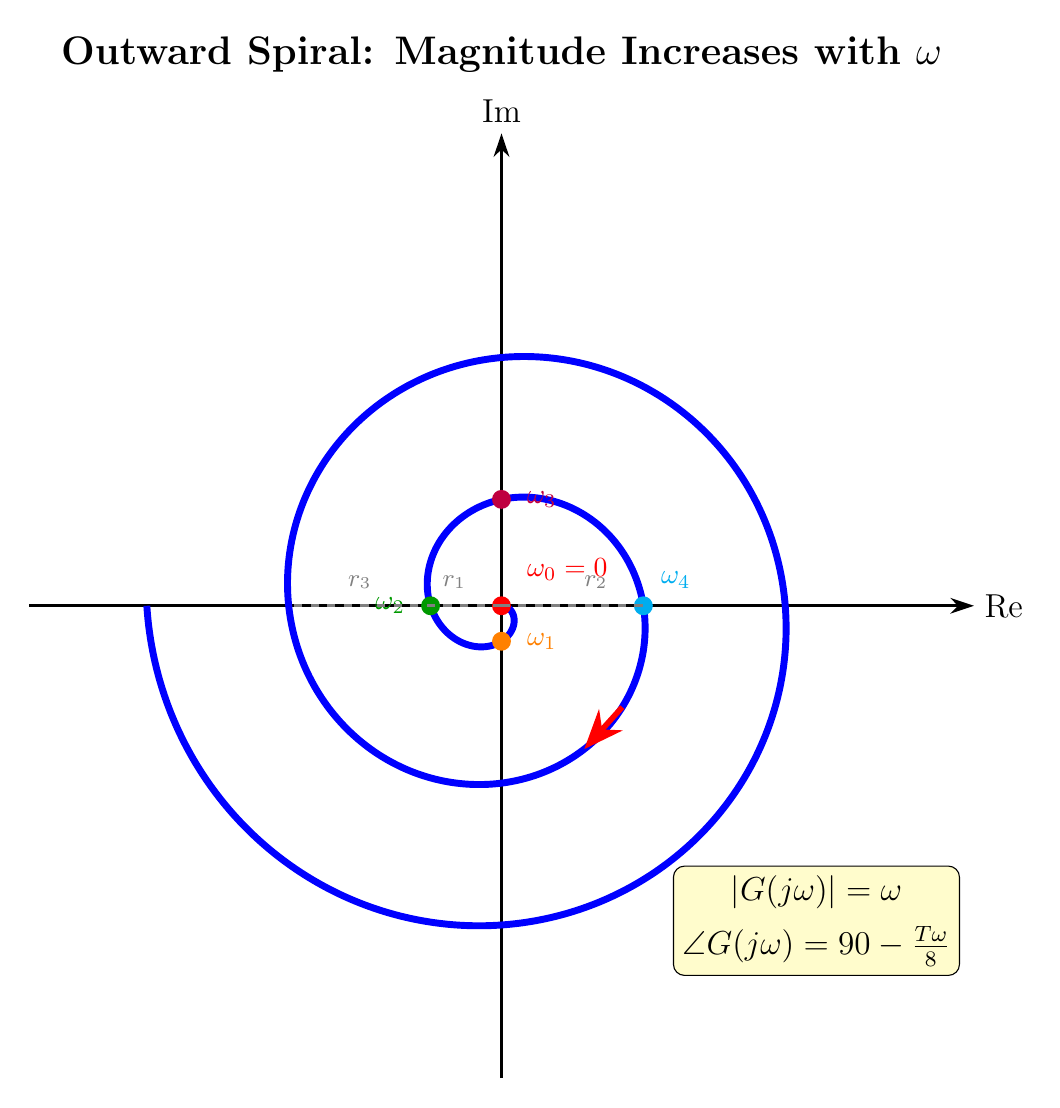
\begin{tikzpicture}[
    arrow/.style={-{Stealth[length=3mm, width=2mm]}, line width=1pt}
]

    % Axes
    \draw[arrow] (-6, 0) -- (6, 0) node[right, font=\large] {Re};
    \draw[arrow] (0, -6) -- (0, 6) node[above, font=\large] {Im};
    
    % Outward spiral
    \draw[line width=2.5pt, blue] plot[domain=0:900, samples=600, smooth] 
        ({0.005*\x*cos(\x)}, {-0.005*\x*sin(\x)});
    
    % Mark specific frequency points
    % ω₁: phase = 0° (on positive real axis)
    \fill[red] ({0.005*0*cos(0)}, {-0.005*0*sin(0)}) circle (0.12);
    \node[above right, red, font=\normalsize] at (0.2, 0.2) {$\omega_0 = 0$};
    
    % ω₂: phase = -90° 
    \fill[orange] ({0.005*90*cos(90)}, {-0.005*90*sin(90)}) circle (0.12);
    \node[right, orange, font=\normalsize] at ({0.005*90*cos(90)+0.2}, {-0.005*90*sin(90)}) {$\omega_1$};
    
    % ω₃: phase = -180°
    \fill[green!60!black] ({0.005*180*cos(180)}, {-0.005*180*sin(180)}) circle (0.12);
    \node[left, green!60!black, font=\normalsize] at ({0.005*180*cos(180)-0.2}, {-0.005*180*sin(180)}) {$\omega_2$};
    
    % ω₄: phase = -270°
    \fill[purple] ({0.005*270*cos(270)}, {-0.005*270*sin(270)}) circle (0.12);
    \node[right, purple, font=\normalsize] at ({0.005*270*cos(270)+0.2}, {-0.005*270*sin(270)}) {$\omega_3$};
    
    % ω₅: phase = -360°
    \fill[cyan] ({0.005*360*cos(360)}, {-0.005*360*sin(360)}) circle (0.12);
    \node[above right, cyan, font=\normalsize] at ({0.005*360*cos(360)+0.1}, {-0.005*360*sin(360)+0.1}) {$\omega_4$};
    
    % Radius lines to show increasing magnitude
    \draw[dashed, gray, line width=1pt] (0, 0) -- ({0.005*180*cos(180)}, {-0.005*180*sin(180)});
    \draw[dashed, gray, line width=1pt] (0, 0) -- ({0.005*360*cos(360)}, {-0.005*360*sin(360)});
    \draw[dashed, gray, line width=1pt] (0, 0) -- ({0.005*540*cos(540)}, {-0.005*540*sin(540)});
    
    % Magnitude labels
    \node[gray, font=\small] at (-0.6, 0.3) {$r_1$};
    \node[gray, font=\small] at (1.2, 0.3) {$r_2$};
    \node[gray, font=\small] at (-1.8, 0.3) {$r_3$};
    
    % Direction arrow
    \draw[-{Stealth[length=5mm, width=4mm]}, red, line width=2pt] 
        ({0.005*400*cos(400)}, {-0.005*400*sin(400)}) -- 
        ({0.005*420*cos(420)}, {-0.005*420*sin(420)});
    
    % Title
    \node[font=\Large\bfseries] at (0, 7) {Outward Spiral: Magnitude Increases with $\omega$};
    
    % Equation box
    \node[draw, fill=yellow!20, rounded corners, font=\large, align=center] at (4, -4) {
        $|G(j\omega)| = \omega$\\[0.2cm]
        $\angle G(j\omega) = 90° - \frac{T\omega}{8}$
    };

\end{tikzpicture}
\caption{Detailed outward spiral showing increasing magnitude with frequency.}
\end{figure}

\newpage

% =============================================================================
% Figure 4: Physical Interpretation
% =============================================================================
\begin{figure}[h]
\centering
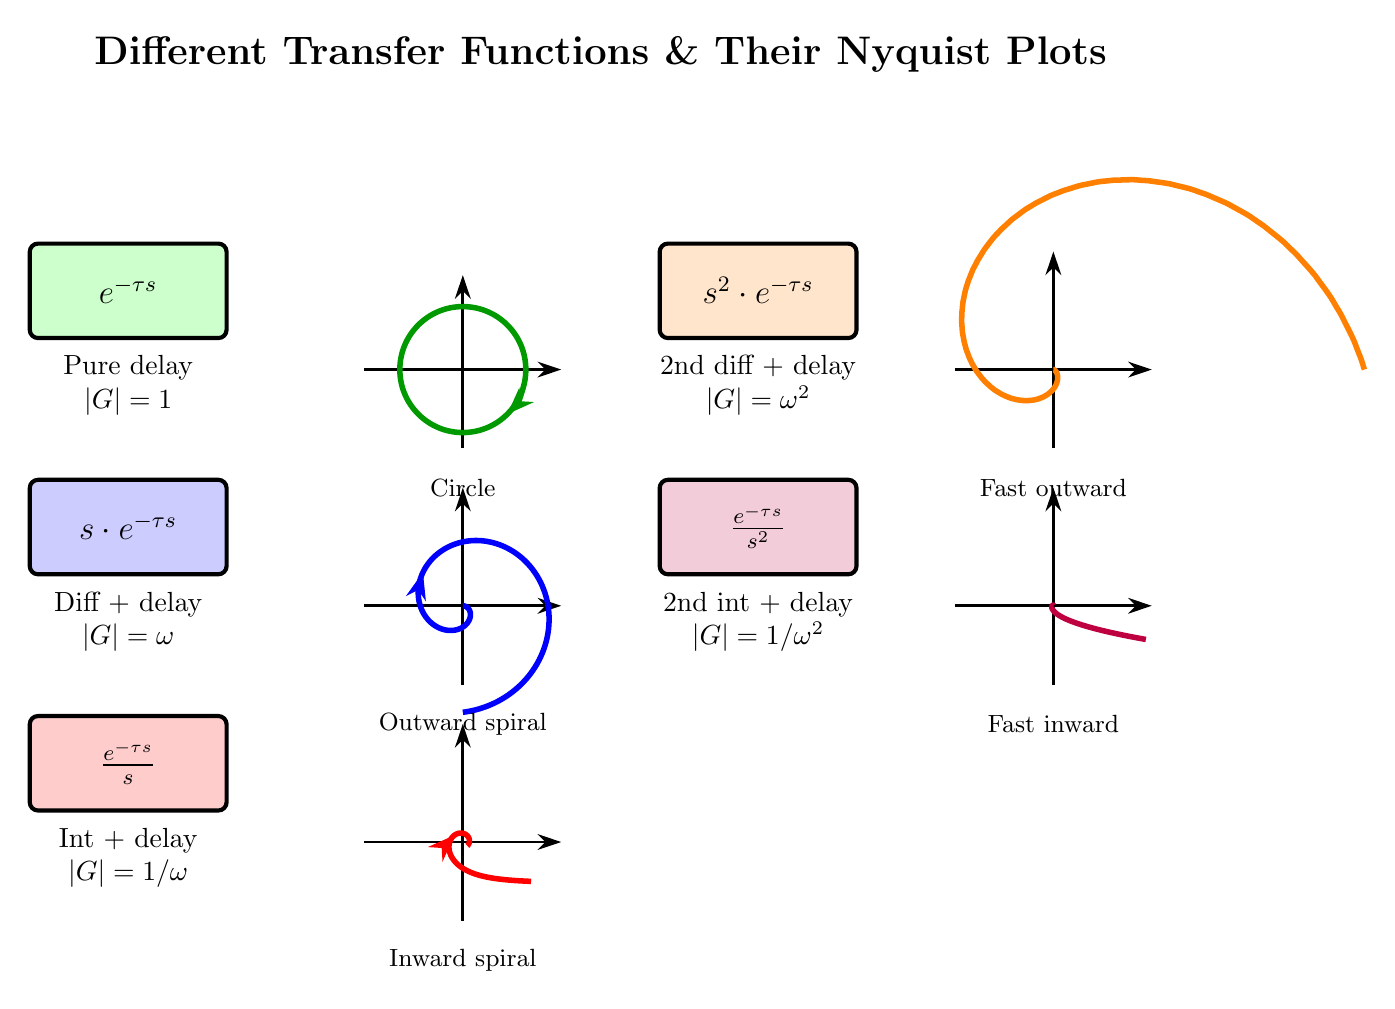
\begin{tikzpicture}[
    arrow/.style={-{Stealth[length=3mm, width=2mm]}, line width=1pt},
    block/.style={rectangle, draw=black, line width=1.5pt, minimum width=2.5cm, 
                  minimum height=1.2cm, font=\large, rounded corners=3pt}
]

    % Title
    \node[font=\Large\bfseries] at (6, 6) {Different Transfer Functions \& Their Nyquist Plots};
    
    % === Case 1: Pure delay (circle) ===
    \begin{scope}[shift={(0, 3)}]
        \node[block, fill=green!20] at (0, 0) {$e^{-\tau s}$};
        \node[font=\normalsize, align=center] at (0, -1.2) {Pure delay\\$|G| = 1$};
        
        % Small Nyquist plot
        \draw[arrow] (3, -1) -- (5.5, -1);
        \draw[arrow] (4.25, -2) -- (4.25, 0.2);
        \draw[line width=2pt, green!60!black] (4.25, -1) circle (0.8);
        \draw[-{Stealth}, green!60!black, line width=1.5pt] (5.05, -1) arc (0:-45:0.8);
        \node[font=\small] at (4.25, -2.5) {Circle};
    \end{scope}
    
    % === Case 2: Differentiator × delay (outward spiral) ===
    \begin{scope}[shift={(0, 0)}]
        \node[block, fill=blue!20] at (0, 0) {$s \cdot e^{-\tau s}$};
        \node[font=\normalsize, align=center] at (0, -1.2) {Diff + delay\\$|G| = \omega$};
        
        % Small Nyquist plot
        \draw[arrow] (3, -1) -- (5.5, -1);
        \draw[arrow] (4.25, -2) -- (4.25, 0.5);
        \draw[line width=2pt, blue] plot[domain=0:450, samples=200, smooth] 
            ({4.25 + 0.003*\x*cos(\x)}, {-1 - 0.003*\x*sin(\x)});
        \draw[-{Stealth}, blue, line width=1.5pt] 
            ({4.25 + 0.003*200*cos(200)}, {-1 - 0.003*200*sin(200)}) --
            ({4.25 + 0.003*220*cos(220)}, {-1 - 0.003*220*sin(220)});
        \node[font=\small] at (4.25, -2.5) {Outward spiral};
    \end{scope}
    
    % === Case 3: Integrator × delay (inward spiral) ===
    \begin{scope}[shift={(0, -3)}]
        \node[block, fill=red!20] at (0, 0) {$\frac{e^{-\tau s}}{s}$};
        \node[font=\normalsize, align=center] at (0, -1.2) {Int + delay\\$|G| = 1/\omega$};
        
        % Small Nyquist plot
        \draw[arrow] (3, -1) -- (5.5, -1);
        \draw[arrow] (4.25, -2) -- (4.25, 0.5);
        \draw[line width=2pt, red] plot[domain=30:400, samples=200, smooth] 
            ({4.25 + 30/\x*cos(\x)}, {-1 - 30/\x*sin(\x)});
        \draw[-{Stealth}, red, line width=1.5pt] 
            ({4.25 + 30/200*cos(200)}, {-1 - 30/200*sin(200)}) --
            ({4.25 + 30/220*cos(220)}, {-1 - 30/220*sin(220)});
        \node[font=\small] at (4.25, -2.5) {Inward spiral};
    \end{scope}
    
    % === Case 4: Second-order × delay ===
    \begin{scope}[shift={(8, 3)}]
        \node[block, fill=orange!20] at (0, 0) {$s^2 \cdot e^{-\tau s}$};
        \node[font=\normalsize, align=center] at (0, -1.2) {2nd diff + delay\\$|G| = \omega^2$};
        
        % Small Nyquist plot
        \draw[arrow] (2.5, -1) -- (5, -1);
        \draw[arrow] (3.75, -2) -- (3.75, 0.5);
        \draw[line width=2pt, orange] plot[domain=0:360, samples=200, smooth] 
            ({3.75 + 0.00003*\x*\x*cos(\x)}, {-1 - 0.00003*\x*\x*sin(\x)});
        \node[font=\small] at (3.75, -2.5) {Fast outward};
    \end{scope}
    
    % === Case 5: Double integrator × delay ===
    \begin{scope}[shift={(8, 0)}]
        \node[block, fill=purple!20] at (0, 0) {$\frac{e^{-\tau s}}{s^2}$};
        \node[font=\normalsize, align=center] at (0, -1.2) {2nd int + delay\\$|G| = 1/\omega^2$};
        
        % Small Nyquist plot
        \draw[arrow] (2.5, -1) -- (5, -1);
        \draw[arrow] (3.75, -2) -- (3.75, 0.5);
        \draw[line width=2pt, purple] plot[domain=20:300, samples=200, smooth] 
            ({3.75 + 500/\x/\x*cos(\x)}, {-1 - 500/\x/\x*sin(\x)});
        \node[font=\small] at (3.75, -2.5) {Fast inward};
    \end{scope}

\end{tikzpicture}
\caption{Different transfer functions and their corresponding Nyquist plot shapes.}
\end{figure}

% =============================================================================
% Summary Table
% =============================================================================
\section{Summary}

\begin{table}[h]
\centering
\renewcommand{\arraystretch}{2}
\begin{tabular}{cccc}
\hline
\textbf{Transfer Function} & \textbf{Magnitude} & \textbf{Nyquist Shape} & \textbf{Direction} \\
\hline
$e^{-\tau s}$ & $1$ (constant) & Circle & Clockwise \\
$s \cdot e^{-\tau s}$ & $\omega$ (linear $\uparrow$) & Outward spiral & Clockwise \\
$s^2 \cdot e^{-\tau s}$ & $\omega^2$ (quadratic $\uparrow$) & Fast outward spiral & Clockwise \\
$\frac{e^{-\tau s}}{s}$ & $\frac{1}{\omega}$ (decreasing) & Inward spiral & Clockwise \\
$\frac{e^{-\tau s}}{s^2}$ & $\frac{1}{\omega^2}$ (fast decreasing) & Fast inward spiral & Clockwise \\
\hline
\end{tabular}
\caption{Summary of different transfer functions and their Nyquist plots.}
\end{table}

% =============================================================================
\section{Block Diagram Analysis}
% =============================================================================

\subsection{Signal Flow in the Control System}

% TikZ: Main Block Diagram
\begin{figure}[h]
\centering
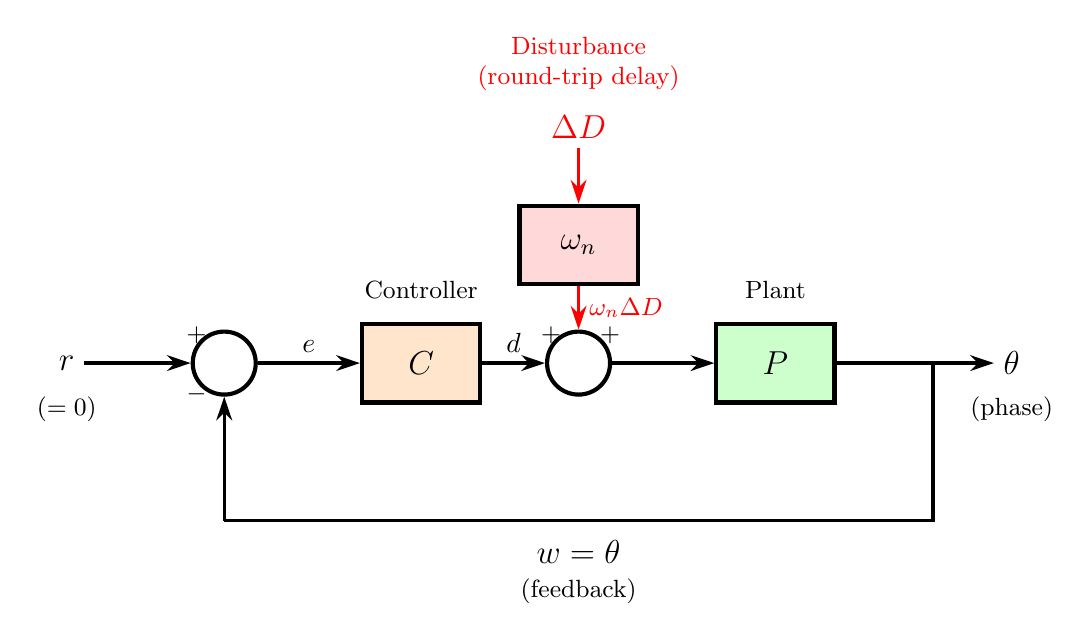
\begin{tikzpicture}[
    block/.style={rectangle, draw=black, line width=1.5pt, minimum width=1.5cm, 
                  minimum height=1cm, font=\large},
    sum/.style={circle, draw=black, line width=1.5pt, minimum size=0.8cm},
    arrow/.style={-{Stealth[length=3mm, width=2mm]}, line width=1.2pt},
    label/.style={font=\large}
]

    % Disturbance input
    \node[label, red] (dist) at (6.5, 3) {$\Delta D$};
    \node[font=\small, red, align=center] at (6.5, 3.8) {Disturbance\\(round-trip delay)};
    
    % Omega_n block
    \node[block, fill=red!15] (wn) at (6.5, 1.5) {$\omega_n$};
    
    % Sum for disturbance
    \node[sum] (sum2) at (6.5, 0) {};
    \node[font=\small] at (6.15, 0.35) {$+$};
    \node[font=\small] at (6.9, 0.35) {$+$};
    
    % Reference input
    \node[label] (input) at (0, 0) {$r$};
    \node[font=\small, below] at (0, -0.3) {$(=0)$};
    
    % Error sum
    \node[sum] (sum1) at (2, 0) {};
    \node[font=\small] at (1.65, 0.35) {$+$};
    \node[font=\small] at (1.65, -0.4) {$-$};
    
    % Controller
    \node[block, fill=orange!20] (C) at (4.5, 0) {$C$};
    \node[font=\small, above] at (4.5, 0.7) {Controller};
    
    % Plant
    \node[block, fill=green!20] (P) at (9, 0) {$P$};
    \node[font=\small, above] at (9, 0.7) {Plant};
    
    % Output
    \node[label] (output) at (12, 0) {$\theta$};
    \node[font=\small, below] at (12, -0.3) {(phase)};
    
    % Forward path arrows
    \draw[arrow] (input) -- (sum1);
    \draw[arrow] (sum1) -- (C) node[midway, above] {$e$};
    \draw[arrow] (C) -- (sum2) node[midway, above] {$d$};
    \draw[arrow, red] (dist) -- (wn);
    \draw[arrow, red] (wn) -- (sum2) node[midway, right, red, font=\small] {$\omega_n \Delta D$};
    \draw[arrow] (sum2) -- (P);
    \draw[arrow] (P) -- (output);
    
    % Feedback path
    \draw[line width=1.2pt] (11, 0) -- (11, -2) -- (2, -2);
    \draw[arrow] (2, -2) -- (sum1);
    \node[label] at (6.5, -2.4) {$w = \theta$};
    \node[font=\small] at (6.5, -2.9) {(feedback)};

\end{tikzpicture}
\caption{Block diagram of the SIL radar control system with disturbance input.}
\end{figure}

\subsection{Signal Definitions}

\begin{table}[h]
\centering
\renewcommand{\arraystretch}{1.5}
\begin{tabular}{cll}
\toprule
\textbf{Signal} & \textbf{Symbol} & \textbf{Physical Meaning} \\
\midrule
Reference & $r$ & Desired phase (set to 0) \\
Error & $e$ & Phase error signal \\
Control output & $d$ & Tunable delay adjustment \\
Disturbance & $\Delta D$ & Round-trip delay change from target motion \\
Output & $\theta$ & Actual phase \\
Feedback & $w$ & Measured phase (= $\theta$) \\
\bottomrule
\end{tabular}
\caption{Signal definitions in the control system.}
\end{table}

% =============================================================================
\section{System Equations}
% =============================================================================

From the block diagram, we can write the following equations:

\subsection{Basic Signal Relationships}

\begin{align}
e &= r - w \label{eq:error}\\
d &= C \cdot e \label{eq:controller}\\
\theta &= P \cdot (d + \omega_n \Delta D) \label{eq:plant}\\
w &= \theta \label{eq:feedback}
\end{align}

% TikZ: Signal Flow Visualization
\begin{figure}[h]
\centering
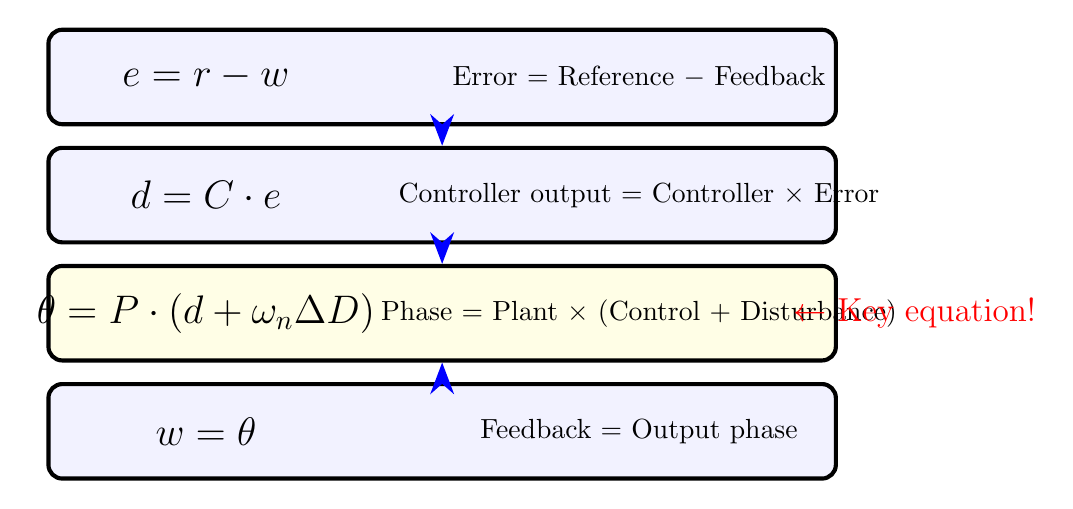
\begin{tikzpicture}[
    box/.style={rectangle, draw=black, line width=1.5pt, rounded corners=5pt,
                minimum width=10cm, minimum height=1.2cm, fill=blue!5},
    arrow/.style={-{Stealth[length=4mm, width=3mm]}, line width=1.5pt}
]

    % Equation 1
    \node[box] (eq1) at (0, 4.5) {};
    \node[font=\Large] at (-3, 4.5) {$e = r - w$};
    \node[font=\normalsize, align=left] at (2.5, 4.5) {Error = Reference $-$ Feedback};
    
    % Equation 2
    \node[box] (eq2) at (0, 3) {};
    \node[font=\Large] at (-3, 3) {$d = C \cdot e$};
    \node[font=\normalsize, align=left] at (2.5, 3) {Controller output = Controller $\times$ Error};
    
    % Equation 3
    \node[box, fill=yellow!10] (eq3) at (0, 1.5) {};
    \node[font=\Large] at (-3, 1.5) {$\theta = P \cdot (d + \omega_n \Delta D)$};
    \node[font=\normalsize, align=left] at (2.5, 1.5) {Phase = Plant $\times$ (Control + Disturbance)};
    
    % Equation 4
    \node[box] (eq4) at (0, 0) {};
    \node[font=\Large] at (-3, 0) {$w = \theta$};
    \node[font=\normalsize, align=left] at (2.5, 0) {Feedback = Output phase};
    
    % Arrows showing flow
    \draw[arrow, blue] (eq1.south) -- (eq2.north);
    \draw[arrow, blue] (eq2.south) -- (eq3.north);
    \draw[arrow, blue] (eq4.north) -- (eq3.south);
    
    % Key equation highlight
    \node[font=\large, red] at (6, 1.5) {$\leftarrow$ Key equation!};

\end{tikzpicture}
\caption{System equations derived from the block diagram.}
\end{figure}

\subsection{Why $\theta = P \cdot (d + \omega_n \Delta D)$?}

This equation comes from the \textbf{physics of the system}:

% TikZ: Physical Interpretation
\begin{figure}[h]
\centering
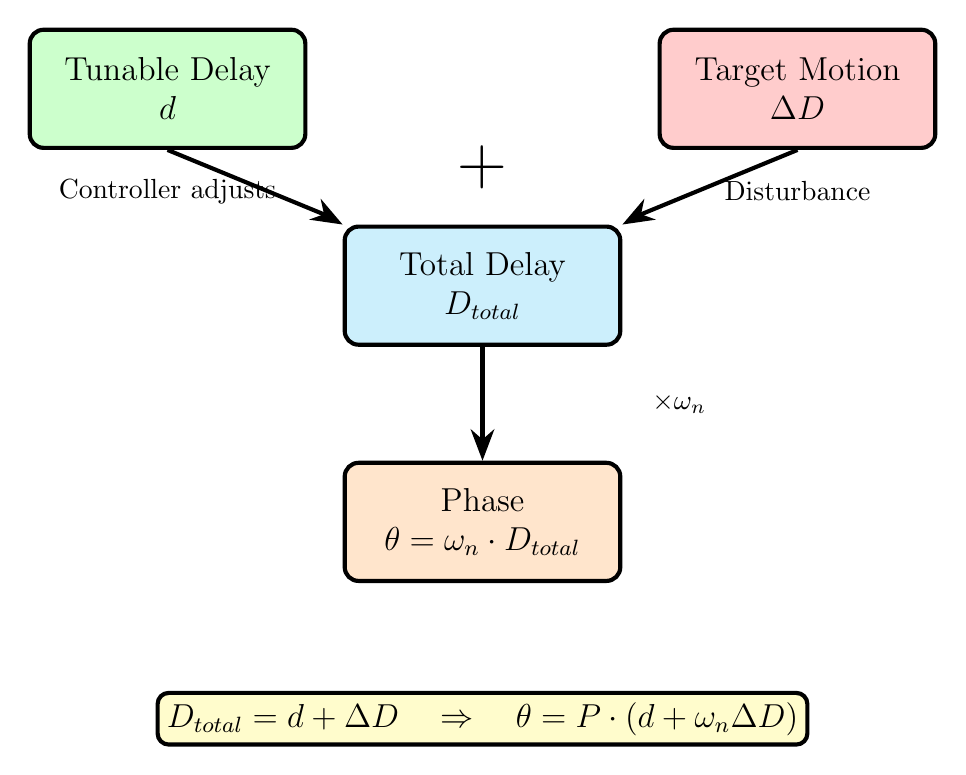
\begin{tikzpicture}[
    block/.style={rectangle, draw=black, line width=1.5pt, rounded corners=5pt,
                  minimum width=3.5cm, minimum height=1.5cm, font=\large, align=center},
    arrow/.style={-{Stealth[length=4mm, width=3mm]}, line width=1.5pt}
]

    % Total delay
    \node[block, fill=cyan!20] (delay) at (0, 0) {Total Delay\\$D_{total}$};
    
    % Components
    \node[block, fill=green!20] (d) at (-4, 2.5) {Tunable Delay\\$d$};
    \node[block, fill=red!20] (deltaD) at (4, 2.5) {Target Motion\\$\Delta D$};
    
    % Conversion to phase
    \node[block, fill=orange!20] (phase) at (0, -3) {Phase\\$\theta = \omega_n \cdot D_{total}$};
    
    % Arrows
    \draw[arrow] (d.south) -- (-2, 0.9) -- (delay.north west);
    \draw[arrow] (deltaD.south) -- (2, 0.9) -- (delay.north east);
    \draw[arrow] (delay.south) -- (phase.north);
    
    % Plus signs
    \node[font=\Huge] at (0, 1.5) {$+$};
    
    % Labels
    \node[font=\normalsize] at (-4, 1.2) {Controller adjusts};
    \node[font=\normalsize] at (4, 1.2) {Disturbance};
    \node[font=\normalsize] at (2.5, -1.5) {$\times \omega_n$};
    
    % Final equation
    \node[draw, fill=yellow!20, rounded corners, font=\large, line width=1.5pt] at (0, -5.5) {
        $D_{total} = d + \Delta D \quad \Rightarrow \quad \theta = P \cdot (d + \omega_n \Delta D)$
    };

\end{tikzpicture}
\caption{Physical interpretation: both control and disturbance affect the total delay.}
\end{figure}

The phase $\theta$ depends on the \textbf{total round-trip delay}:
\begin{equation}
\theta = \omega_n \times (\text{total delay}) = \omega_n (D_0 + d + \Delta D)
\end{equation}

At the operating point, $\omega_n D_0 = \pi$, so the deviation is:
\begin{equation}
\theta - \pi = \omega_n (d + \Delta D)
\end{equation}

Through the SIL dynamics (plant $P$):
\begin{equation}
\boxed{\theta = P \cdot (d + \omega_n \Delta D)}
\end{equation}

% =============================================================================
\section{Derivation of Transfer Function}
% =============================================================================

\subsection{Step-by-Step Derivation}

% TikZ: Derivation Steps
\begin{figure}[h]
\centering
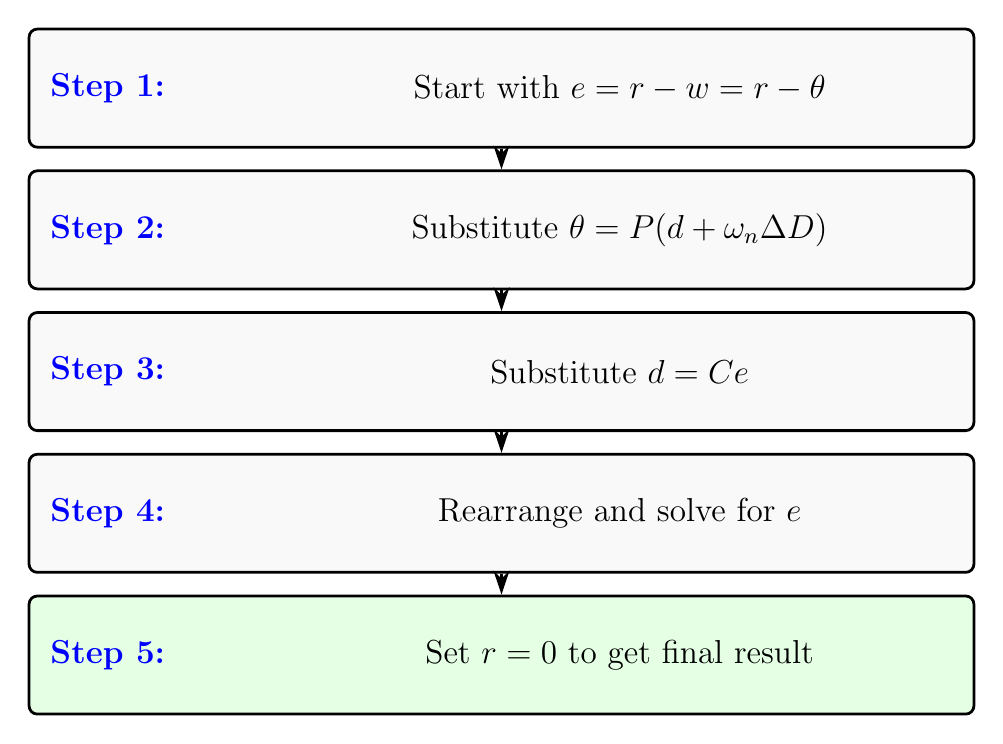
\begin{tikzpicture}[
    stepbox/.style={rectangle, draw=black, line width=1pt, rounded corners=3pt,
                    minimum width=12cm, minimum height=1.5cm, fill=gray!5},
    arrow/.style={-{Stealth[length=3mm, width=2mm]}, line width=1.2pt}
]

    % Step 1
    \node[stepbox] (s1) at (0, 6) {};
    \node[font=\large\bfseries, blue] at (-5, 6) {Step 1:};
    \node[font=\large] at (1.5, 6) {Start with $e = r - w = r - \theta$};
    
    % Step 2
    \node[stepbox] (s2) at (0, 4.2) {};
    \node[font=\large\bfseries, blue] at (-5, 4.2) {Step 2:};
    \node[font=\large] at (1.5, 4.2) {Substitute $\theta = P(d + \omega_n \Delta D)$};
    
    % Step 3
    \node[stepbox] (s3) at (0, 2.4) {};
    \node[font=\large\bfseries, blue] at (-5, 2.4) {Step 3:};
    \node[font=\large] at (1.5, 2.4) {Substitute $d = Ce$};
    
    % Step 4
    \node[stepbox] (s4) at (0, 0.6) {};
    \node[font=\large\bfseries, blue] at (-5, 0.6) {Step 4:};
    \node[font=\large] at (1.5, 0.6) {Rearrange and solve for $e$};
    
    % Step 5
    \node[stepbox, fill=green!10] (s5) at (0, -1.2) {};
    \node[font=\large\bfseries, blue] at (-5, -1.2) {Step 5:};
    \node[font=\large] at (1.5, -1.2) {Set $r = 0$ to get final result};
    
    % Arrows
    \draw[arrow] (s1.south) -- (s2.north);
    \draw[arrow] (s2.south) -- (s3.north);
    \draw[arrow] (s3.south) -- (s4.north);
    \draw[arrow] (s4.south) -- (s5.north);

\end{tikzpicture}
\caption{Step-by-step derivation procedure.}
\end{figure}

\textbf{Step 1:} Start with the error equation
\begin{equation}
e = r - w = r - \theta
\end{equation}

\textbf{Step 2:} Substitute $\theta = P(d + \omega_n \Delta D)$
\begin{equation}
e = r - P(d + \omega_n \Delta D) = r - Pd - P\omega_n \Delta D
\end{equation}

\textbf{Step 3:} Substitute $d = Ce$
\begin{equation}
e = r - P(Ce) - P\omega_n \Delta D = r - PCe - P\omega_n \Delta D
\end{equation}

\textbf{Step 4:} Rearrange
\begin{equation}
e + PCe = r - P\omega_n \Delta D
\end{equation}
\begin{equation}
e(1 + PC) = r - P\omega_n \Delta D
\end{equation}

\textbf{Step 5:} Solve for $e$ with $r = 0$
\begin{equation}
e = \frac{-P\omega_n \Delta D}{1 + PC}
\end{equation}

\textbf{Wait!} This gives $1 + PC$, but the paper has $1 - PC$. Why?

% =============================================================================
\section{The Sign Convention: Why $1 - PC$?}
% =============================================================================

\subsection{The Plant Has Negative Gain}

From \textbf{equation (9)} in the paper:
\begin{equation}
P(s) = \underbrace{-k}_{\text{negative!}} \cdot e^{-\frac{T}{8}s} \cdot F(s)
\end{equation}

% TikZ: Negative Gain Explanation
\begin{figure}[h]
\centering
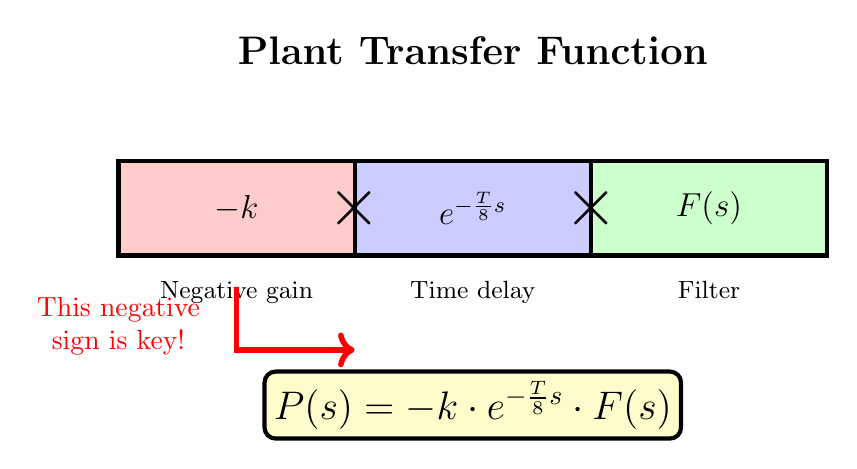
\begin{tikzpicture}[
    block/.style={rectangle, draw=black, line width=1.5pt, minimum width=3cm, 
                  minimum height=1.2cm, font=\large},
    arrow/.style={-{Stealth[length=3mm, width=2mm]}, line width=1.2pt}
]

    % Plant decomposition
    \node[font=\Large\bfseries] at (0, 3) {Plant Transfer Function};
    
    \node[block, fill=red!20] (neg) at (-3, 1) {$-k$};
    \node[font=\small, below] at (-3, 0.2) {Negative gain};
    
    \node[block, fill=blue!20] (delay) at (0, 1) {$e^{-\frac{T}{8}s}$};
    \node[font=\small, below] at (0, 0.2) {Time delay};
    
    \node[block, fill=green!20] (filter) at (3, 1) {$F(s)$};
    \node[font=\small, below] at (3, 0.2) {Filter};
    
    % Multiplication signs
    \node[font=\Huge] at (-1.5, 1) {$\times$};
    \node[font=\Huge] at (1.5, 1) {$\times$};
    
    % Result
    \node[draw, fill=yellow!20, rounded corners, font=\Large, line width=1.5pt] at (0, -1.5) {
        $P(s) = -k \cdot e^{-\frac{T}{8}s} \cdot F(s)$
    };
    
    % Highlight
    \draw[red, line width=2pt, ->] (-3, 0) -- (-3, -0.8) -- (-1.5, -0.8);
    \node[red, font=\normalsize, align=center] at (-4.5, -0.5) {This negative\\sign is key!};

\end{tikzpicture}
\caption{The plant has a negative gain due to anti-phase operation.}
\end{figure}

\subsection{Why is the Gain Negative?}

% TikZ: Anti-phase Mode Explanation
\begin{figure}[h]
\centering
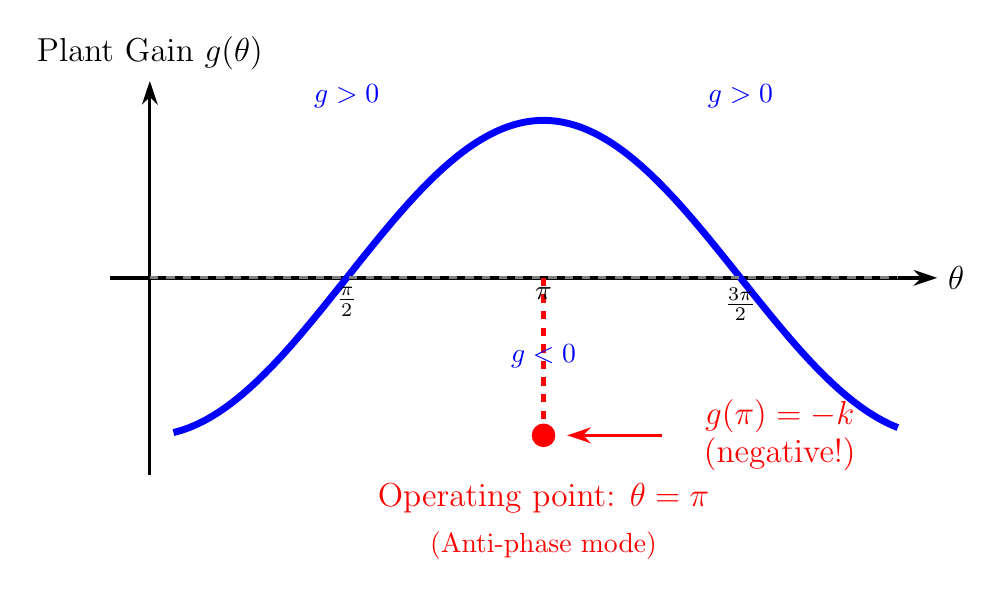
\begin{tikzpicture}[
    arrow/.style={-{Stealth[length=3mm, width=2mm]}, line width=1.2pt}
]

    % Axes for gain curve
    \draw[arrow] (-0.5, 0) -- (10, 0) node[right, font=\large] {$\theta$};
    \draw[arrow] (0, -2.5) -- (0, 2.5) node[above, font=\large] {Plant Gain $g(\theta)$};
    
    % Gain curve (cosine-like)
    \draw[line width=2.5pt, blue] plot[smooth, domain=0.3:9.5, samples=100] 
        (\x, {2*cos((\x-5)*36)});
    
    % Zero line
    \draw[dashed, gray, line width=1pt] (0, 0) -- (9.5, 0);
    
    % Operating point at θ = π
    \fill[red] (5, -2) circle (0.15);
    \draw[red, line width=2pt, dashed] (5, 0) -- (5, -2);
    
    % Labels
    \node[below] at (2.5, 0) {$\frac{\pi}{2}$};
    \node[below] at (5, 0) {$\pi$};
    \node[below] at (7.5, 0) {$\frac{3\pi}{2}$};
    
    % Annotations
    \node[red, font=\large] at (5, -2.8) {Operating point: $\theta = \pi$};
    \node[red, font=\normalsize] at (5, -3.4) {(Anti-phase mode)};
    
    % Gain value annotation
    \draw[arrow, red] (6.5, -2) -- (5.3, -2);
    \node[red, font=\large, align=center] at (8, -2) {$g(\pi) = -k$\\(negative!)};
    
    % Positive region
    \node[blue, font=\normalsize] at (2.5, 2.3) {$g > 0$};
    \node[blue, font=\normalsize] at (7.5, 2.3) {$g > 0$};
    
    % Negative region
    \node[blue, font=\normalsize] at (5, -1) {$g < 0$};

\end{tikzpicture}
\caption{At the operating point $\theta = \pi$, the plant gain is negative.}
\end{figure}

The system operates in \textbf{anti-phase mode} ($\theta = \pi$) where:
\begin{itemize}
    \item The plant gain $g(\theta, A_{inj})$ is \textbf{negative}
    \item This provides better linearity and stability
    \item The negative gain means: increasing delay $\rightarrow$ decreasing phase
\end{itemize}

\subsection{Correcting the Derivation}

Let's write $P = -|P|$ explicitly (negative plant):

\textbf{Step 1:} With explicit negative sign
\begin{equation}
\theta = P(d + \omega_n \Delta D) = (-|P|)(d + \omega_n \Delta D)
\end{equation}

\textbf{Step 2:} Error equation
\begin{equation}
e = r - \theta = r - (-|P|)(d + \omega_n \Delta D) = r + |P|(d + \omega_n \Delta D)
\end{equation}

\textbf{Step 3:} Expand
\begin{equation}
e = r + |P|d + |P|\omega_n \Delta D = r + |P|Ce + |P|\omega_n \Delta D
\end{equation}

\textbf{Step 4:} Rearrange
\begin{equation}
e - |P|Ce = r + |P|\omega_n \Delta D
\end{equation}
\begin{equation}
e(1 - |P|C) = r + |P|\omega_n \Delta D
\end{equation}

\textbf{Step 5:} Solve for $e$ with $r = 0$
\begin{equation}
e = \frac{|P|\omega_n \Delta D}{1 - |P|C}
\end{equation}

If the paper defines $P$ as the \textbf{positive magnitude}:
\begin{equation}
\boxed{e(s) = \frac{P \cdot \omega_n \Delta D(s)}{1 - PC}}
\end{equation}

Or simplifying at low frequencies where $P \approx 1$:
\begin{equation}
\boxed{e(s) = \frac{\omega_n \Delta D(s)}{1 - PC}}
\end{equation}

% =============================================================================
\section{Visual Summary of the Derivation}
% =============================================================================

% TikZ: Complete Derivation Flow
\begin{figure}[h]
\centering
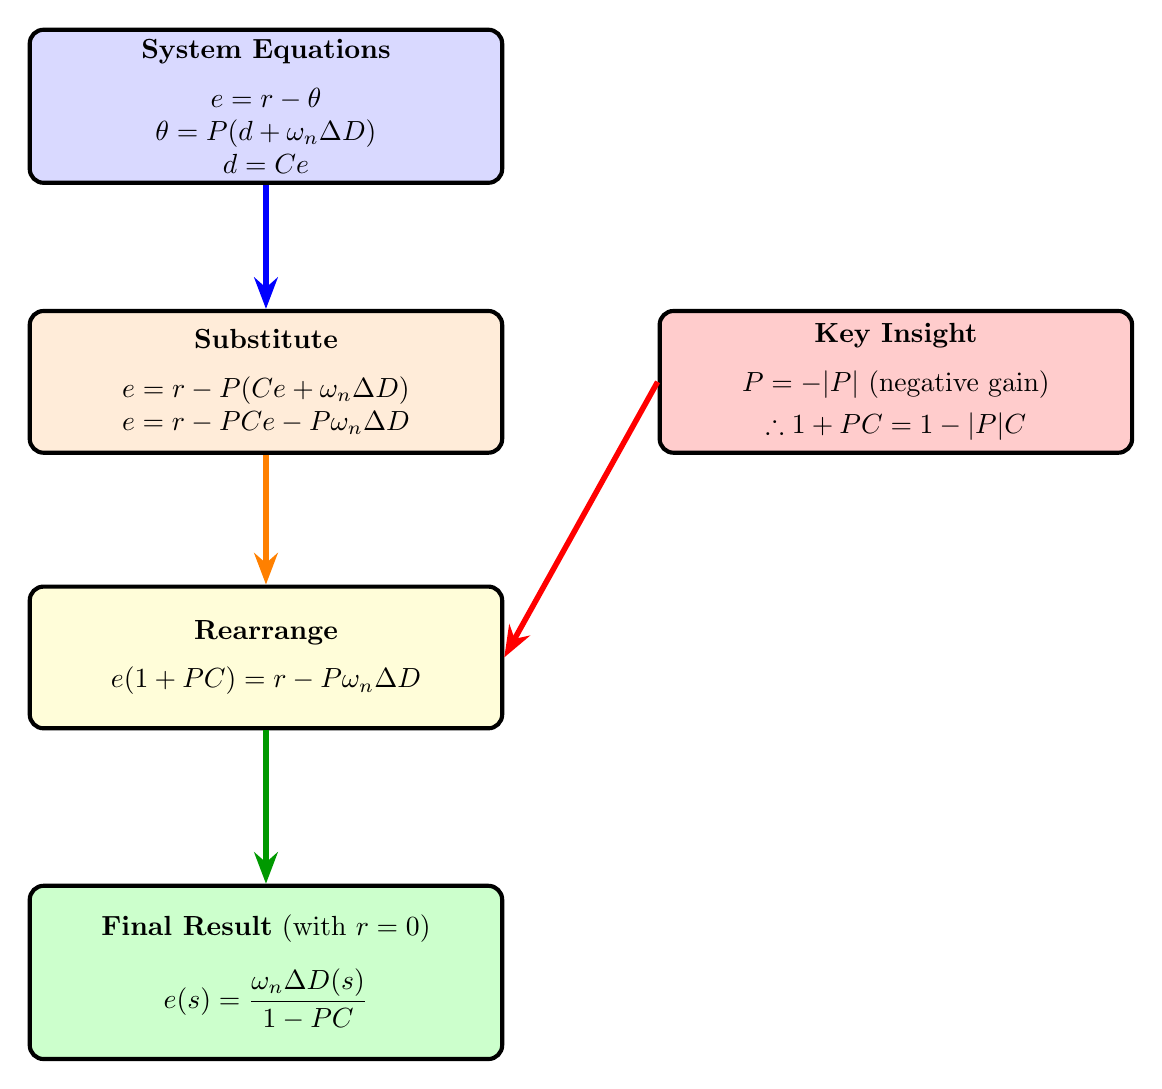
\begin{tikzpicture}[
    box/.style={rectangle, draw=black, line width=1.5pt, rounded corners=5pt,
                minimum width=6cm, minimum height=1.8cm, align=center},
    arrow/.style={-{Stealth[length=4mm, width=3mm]}, line width=2pt}
]

    % Start
    \node[box, fill=blue!15] (start) at (0, 8) {
        \textbf{System Equations}\\[0.2cm]
        $e = r - \theta$\\
        $\theta = P(d + \omega_n \Delta D)$\\
        $d = Ce$
    };
    
    % Substitute
    \node[box, fill=orange!15] (sub) at (0, 4.5) {
        \textbf{Substitute}\\[0.2cm]
        $e = r - P(Ce + \omega_n \Delta D)$\\
        $e = r - PCe - P\omega_n \Delta D$
    };
    
    % Rearrange
    \node[box, fill=yellow!15] (rearr) at (0, 1) {
        \textbf{Rearrange}\\[0.2cm]
        $e(1 + PC) = r - P\omega_n \Delta D$
    };
    
    % Key insight
    \node[box, fill=red!20] (key) at (8, 4.5) {
        \textbf{Key Insight}\\[0.2cm]
        $P = -|P|$ (negative gain)\\[0.1cm]
        $\therefore 1 + PC = 1 - |P|C$
    };
    
    % Final result
    \node[box, fill=green!20, minimum height=2.2cm] (result) at (0, -3) {
        \textbf{Final Result} (with $r = 0$)\\[0.3cm]
        $\displaystyle e(s) = \frac{\omega_n \Delta D(s)}{1 - PC}$
    };
    
    % Arrows
    \draw[arrow, blue] (start.south) -- (sub.north);
    \draw[arrow, orange] (sub.south) -- (rearr.north);
    \draw[arrow, red] (key.west) -- (rearr.east);
    \draw[arrow, green!60!black] (rearr.south) -- (result.north);

\end{tikzpicture}
\caption{Complete derivation flow showing how $1 - PC$ arises from negative plant gain.}
\end{figure}

% =============================================================================
\section{Substituting the PI Controller}
% =============================================================================

The PI controller is:
\begin{equation}
C(s) = k_p + \frac{k_I}{s} = \frac{k_p s + k_I}{s}
\end{equation}

% TikZ: PI Controller Structure
\begin{figure}[h]
\centering
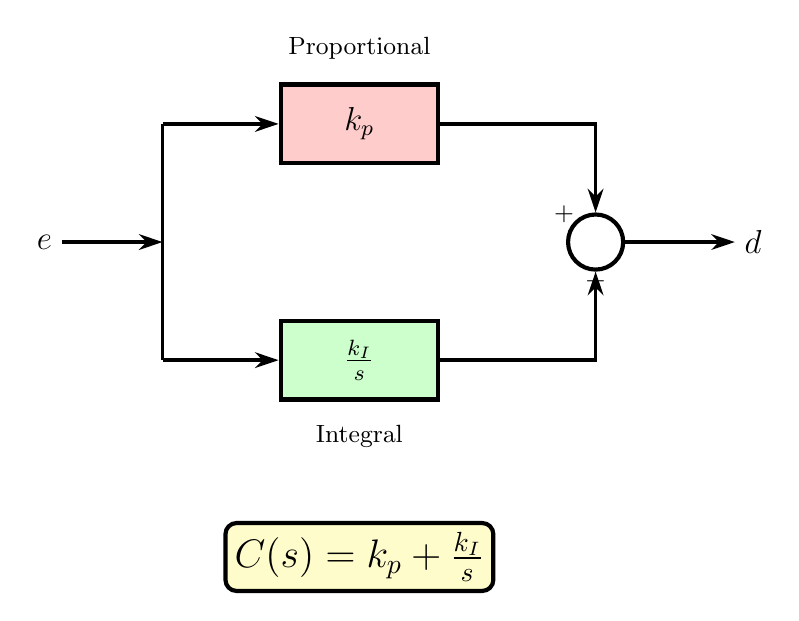
\begin{tikzpicture}[
    block/.style={rectangle, draw=black, line width=1.5pt, minimum width=2cm, 
                  minimum height=1cm, font=\large},
    sum/.style={circle, draw=black, line width=1.5pt, minimum size=0.7cm},
    arrow/.style={-{Stealth[length=3mm, width=2mm]}, line width=1.2pt}
]

    % Input
    \node[font=\large] (input) at (0, 0) {$e$};
    
    % Branch point
    \coordinate (branch) at (1.5, 0);
    
    % Proportional path
    \node[block, fill=red!20] (P) at (4, 1.5) {$k_p$};
    \node[font=\small, above] at (4, 2.2) {Proportional};
    
    % Integral path
    \node[block, fill=green!20] (I) at (4, -1.5) {$\frac{k_I}{s}$};
    \node[font=\small, below] at (4, -2.2) {Integral};
    
    % Sum
    \node[sum] (sum) at (7, 0) {};
    \node[font=\small] at (6.6, 0.35) {$+$};
    \node[font=\small] at (7, -0.5) {$+$};
    
    % Output
    \node[font=\large] (output) at (9, 0) {$d$};
    
    % Arrows
    \draw[arrow] (input) -- (branch);
    \draw[line width=1.2pt] (branch) -- (1.5, 1.5);
    \draw[line width=1.2pt] (branch) -- (1.5, -1.5);
    \draw[arrow] (1.5, 1.5) -- (P);
    \draw[arrow] (1.5, -1.5) -- (I);
    \draw[arrow] (P) -- (7, 1.5) -- (sum);
    \draw[arrow] (I) -- (7, -1.5) -- (sum);
    \draw[arrow] (sum) -- (output);
    
    % Equation
    \node[draw, fill=yellow!20, rounded corners, font=\Large, line width=1.5pt] at (4, -4) {
        $C(s) = k_p + \frac{k_I}{s}$
    };

\end{tikzpicture}
\caption{PI controller structure.}
\end{figure}

Substituting into $1 - PC$:
\begin{align}
1 - PC &= 1 - P \cdot \left(k_p + \frac{k_I}{s}\right)\\
&= 1 - k_p P - \frac{k_I P}{s}
\end{align}

\textbf{Final transfer function:}
\begin{equation}
\boxed{e(s) = \frac{\Delta D(s) \omega_n}{1 - PC} = \frac{\Delta D(s) \omega_n}{1 - k_p P - k_I P/s}}
\end{equation}

This is exactly \textbf{equation (16)} in the paper!

% =============================================================================
\section{Block Diagram Comparison}
% =============================================================================

% TikZ: Standard vs This System Comparison
\begin{figure}[h]
\centering
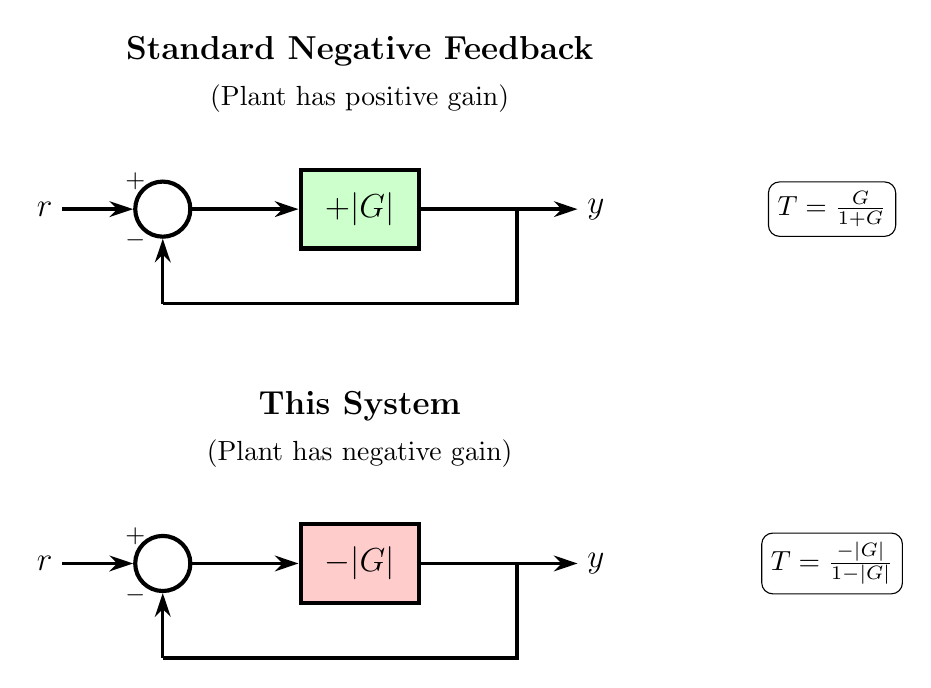
\begin{tikzpicture}[
    block/.style={rectangle, draw=black, line width=1.5pt, minimum width=1.5cm, 
                  minimum height=1cm, font=\large},
    sum/.style={circle, draw=black, line width=1.5pt, minimum size=0.7cm},
    arrow/.style={-{Stealth[length=3mm, width=2mm]}, line width=1.2pt}
]

    % === Standard Negative Feedback ===
    \begin{scope}[shift={(0, 3)}]
        \node[font=\large\bfseries] at (4, 2) {Standard Negative Feedback};
        \node[font=\normalsize] at (4, 1.4) {(Plant has positive gain)};
        
        \node[font=\large] (in1) at (0, 0) {$r$};
        \node[sum] (s1) at (1.5, 0) {};
        \node[font=\small] at (1.15, 0.35) {$+$};
        \node[font=\small] at (1.15, -0.4) {$-$};
        \node[block, fill=green!20] (g1) at (4, 0) {$+|G|$};
        \node[font=\large] (out1) at (7, 0) {$y$};
        
        \draw[arrow] (in1) -- (s1);
        \draw[arrow] (s1) -- (g1);
        \draw[arrow] (g1) -- (out1);
        \draw[line width=1.2pt] (6, 0) -- (6, -1.2) -- (1.5, -1.2);
        \draw[arrow] (1.5, -1.2) -- (s1);
        
        \node[draw, rounded corners, font=\normalsize] at (10, 0) {$T = \frac{G}{1+G}$};
    \end{scope}
    
    % === This System (Negative Plant Gain) ===
    \begin{scope}[shift={(0, -1.5)}]
        \node[font=\large\bfseries] at (4, 2) {This System};
        \node[font=\normalsize] at (4, 1.4) {(Plant has negative gain)};
        
        \node[font=\large] (in2) at (0, 0) {$r$};
        \node[sum] (s2) at (1.5, 0) {};
        \node[font=\small] at (1.15, 0.35) {$+$};
        \node[font=\small] at (1.15, -0.4) {$-$};
        \node[block, fill=red!20] (g2) at (4, 0) {$-|G|$};
        \node[font=\large] (out2) at (7, 0) {$y$};
        
        \draw[arrow] (in2) -- (s2);
        \draw[arrow] (s2) -- (g2);
        \draw[arrow] (g2) -- (out2);
        \draw[line width=1.2pt] (6, 0) -- (6, -1.2) -- (1.5, -1.2);
        \draw[arrow] (1.5, -1.2) -- (s2);
        
        \node[draw, rounded corners, font=\normalsize] at (10, 0) {$T = \frac{-|G|}{1-|G|}$};
    \end{scope}

\end{tikzpicture}
\caption{Comparison: standard feedback vs.\ this system with negative plant gain.}
\end{figure}

% =============================================================================
\section{Summary}
% =============================================================================

\begin{table}[h]
\centering
\renewcommand{\arraystretch}{2}
\begin{tabular}{ll}
\toprule
\textbf{Question} & \textbf{Answer} \\
\midrule
Why $\theta = P(d + \omega_n \Delta D)$? & Both control and disturbance affect total delay \\
Why $1 - PC$ instead of $1 + PC$? & Plant $P$ has \textbf{negative gain} in anti-phase mode \\
Physical meaning & Negative gain: increasing delay $\to$ decreasing phase \\
\bottomrule
\end{tabular}
\caption{Summary of key questions and answers.}
\end{table}

% TikZ: Final Key Message
\begin{figure}[h]
\centering
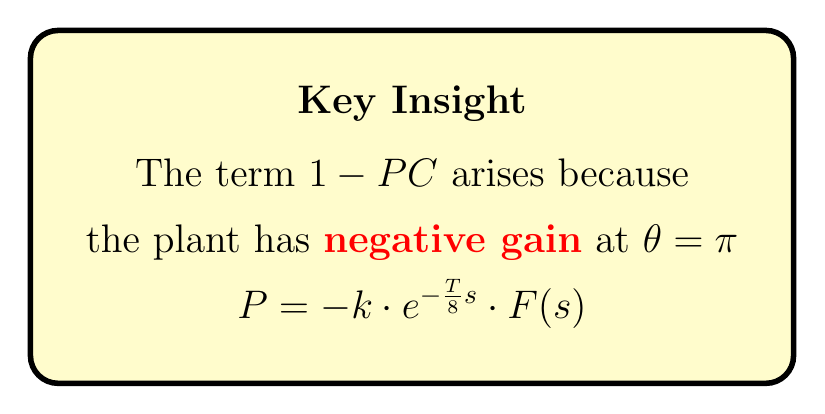
\begin{tikzpicture}
    \node[draw=black, fill=yellow!20, rounded corners=10pt, line width=2pt, 
          font=\Large, inner sep=20pt, align=center] at (0, 0) {
        \textbf{Key Insight}\\[0.3cm]
        The term $1 - PC$ arises because\\[0.2cm]
        the plant has \textcolor{red}{\textbf{negative gain}} at $\theta = \pi$\\[0.2cm]
        $P = -k \cdot e^{-\frac{T}{8}s} \cdot F(s)$
    };
\end{tikzpicture}
\end{figure}




\end{document}